\documentclass[a4paper,11pt]{article}
\usepackage[table]{xcolor}



\newcommand{\defeq}{\mathrel{\doteq}}

\newcommand{\lzero}{0}

\newcommand{\kw}[1]{\mathtt{#1}}

\newcommand{\expr}{e}
\newcommand{\vall}{w}
\newcommand{\valr}{v}
\newcommand{\eif}{\kw{if}}
\newcommand{\eapp}{\;}
\newcommand{\eprojl}{\kw{fst}}
\newcommand{\eprojr}{\kw{snd}}
%\newcommand{\eprov}[1]{\eta_{#1}}
\newcommand{\etrue}{\kw{true}}
\newcommand{\efalse}{\kw{false}}
\newcommand{\econst}{c}
\newcommand{\eop}{\delta}
\newcommand{\efix}{\mathop{\kw{fix}}}
%\newcommand{\labelA}{\ell}

\newcommand{\tr}{T}
\newcommand{\trift}{\eif^{\kw{t}}}
\newcommand{\triff}{\eif^{\kw{f}}}
\newcommand{\trprojl}{\eprojl}
\newcommand{\trprojr}{\eprojr}
\newcommand{\trtrue}{\etrue}
\newcommand{\trfalse}{\efalse}
\newcommand{\trconst}{\econst}
\newcommand{\trop}{\eop}
\newcommand{\trfix}{\efix}
\newcommand{\trapp}[5]{#1 \; #2 \mathrel{\triangleright} {\efix #3(#4).#5}}

\newcommand{\adap}{\kw{adap}}
\newcommand{\ddep}[1]{\kw{depth}_{#1}}
\newcommand{\nat}{\mathbb{N}}
\newcommand{\natb}{\nat_{\bot}}
\newcommand{\natbi}{\natb^\infty}
\newcommand{\nnatA}{n}
\newcommand{\nnatB}{m}
\newcommand{\nnatbA}{s}
\newcommand{\nnatbB}{t}
\newcommand{\nnatbiA}{q}
\newcommand{\nnatbiB}{r}

\newcommand{\type}{\tau}
\newcommand{\tbase}{\kw{b}}
\newcommand{\tbool}{\kw{bool}}
\newcommand{\tarr}[5]{#1; #3 \xrightarrow{#4; \, #5} #2}
\newcommand{\env}{\theta}

\newcommand{\bigstep}{\mathrel{\Downarrow}}

\newcommand{\dmap}{\rho}
\newcommand{\dmapb}{\bot_\dmap}
\newcommand{\supp}{\kw{supp}}
\newcommand{\dom}{\kw{dom}}

\newcommand{\tvdash}[1]{\vdash_{#1}}

%Packages
\usepackage[T1]{fontenc}
\usepackage{fourier} 
\usepackage[english]{babel} 
\usepackage{amsmath,amsfonts} 
\usepackage{amsthm} 
\usepackage{color}   %May be necessary if you want to color links
\usepackage{hyperref}
\usepackage{lscape}
\usepackage{geometry}
\usepackage{amsmath}
\usepackage{algorithm}
\usepackage{algorithmic}
\usepackage{amssymb}
\usepackage{amsfonts}
\usepackage{times}
\usepackage{bm}
\usepackage{ stmaryrd }
\SetSymbolFont{stmry}{bold}{U}{stmry}{m}{n}

\usepackage{ amssymb }
\usepackage{ textcomp }
\usepackage[normalem]{ulem}
% For derivation rules
\usepackage{mathpartir}
\usepackage{color}
\usepackage{a4wide}
\usepackage{caption}
\usepackage{subcaption}
\usepackage{mathpartir}
\usepackage{amsmath,amsfonts}
\usepackage{ amssymb }
\usepackage{color}
\usepackage{algorithm}
\usepackage{algorithmic}
\usepackage{microtype}
\usepackage{eucal}
\usepackage{url}
\usepackage{xspace}
\usepackage{array}
\usepackage{listings}

\usepackage{tikz}
\usetikzlibrary{shapes.geometric}
\usetikzlibrary{arrows.meta,arrows}
\usetikzlibrary{decorations.text}
% % % % 


\usepackage{multirow}


%%%%%%%%%%%%%%%%%%%%%%%%%%%%%%%%%%%%%%%%%%%%%%%%%%%%%Packages And Definitions For Listing the Code%%%%%%%%%%%%%%%%%%%%%%%%%%%%%%%%%%%%%%%%%%%%%%%%%%%%%%%%%%%%%%%%%%%%%%%%
\usepackage{listings}
\usepackage{xcolor}

\definecolor{codegreen}{rgb}{0,0.6,0}
\definecolor{codegray}{rgb}{0.5,0.5,0.5}
\definecolor{codepurple}{rgb}{0.58,0,0.82}
\definecolor{backcolour}{rgb}{0.95,0.95,0.92}

\lstdefinestyle{mystyle}{
    backgroundcolor=\color{backcolour},   
    commentstyle=\color{codegreen},
    keywordstyle=\color{magenta},
    numberstyle=\tiny\color{codegray},
    stringstyle=\color{codepurple},
    basicstyle=\ttfamily\footnotesize,
    breakatwhitespace=false,         
    breaklines=true,                 
    captionpos=b,                    
    keepspaces=true,                 
    numbers=left,                    
    numbersep=5pt,                  
    showspaces=false,                
    showstringspaces=false,
    showtabs=false,                  
    tabsize=2
}

\lstset{style=mystyle}

\usepackage{tikz}
\usetikzlibrary{shapes,arrows}
\newcommand{\THESYSTEM}{\textsf{AdaptFun}}

% Define block styles
\tikzstyle{decision} = [diamond, draw, fill=blue!20, 
    text width=4.5em, text badly centered, node distance=3cm, inner sep=0pt]
\tikzstyle{block} = [rectangle, draw, fill=blue!20, 
    text width=5em, text centered, rounded corners, minimum height=4em]
\tikzstyle{line} = [draw, -latex']
\tikzstyle{cloud} = [draw, ellipse,fill=red!20, node distance=3cm,
    minimum height=2em]

\begin{document}
\title{Appendix for "Program Analysis for Adaptivity Analysis"}

\author{}

\date{}

\maketitle

In this appendix, we present the full details of the 2 languages: while language and the SSA language.

\tableofcontents


% \section{Introduction}
\section{System Overview}


In adaptive data analysis, a data analysis can depend on the results of
previous analysis over the same data. This dependency may affect the
\emph{generalization properties of the data analysis}. To study this phenomenon
in a formal way, we consider the \emph{statistical query
  model}. In this model, a dataset $X$ consisting of $d$ attributes (columns) and $n$
individuals' data (rows) can be accessed only through an interface to
which one can submit statistical queries. More precisely, suppose that
the type of a row is $R$ (as an example, a row with $d$ binary
attributes would have type $R=\{0,1\}^d$. Then, in the statistical
query model one can access the dataset only by submitting a query to
the interface, in
the form of a function
$p:D\to [0,1] $ where $D$ represents dataset. The collected answer of
the asked query is the average result of $p$ on each row in the
dataset $D$. For example, the result is the
value $\frac{1}{n}\sum_{i=1}^n p(X_i)$ where
$X_i$ is the row of index $i$ in $X$. While this model is rather
simple, in fact it supports sufficient statistics one may be
interested.

 

We are interested in the adaptivity of mechanisms in the model, which is straightforward supported by a high level language. In this language, queries are allowed to carry arguments to simulate the process of submitting a query to the interface in
the model, for example, the expression $\query(e)$ tells us the argument $e$ is consumed to construct the
query. To be precise, one submitted query who needs the average of
answers of previous queries is expressed as $\query(x)$, where the variable $x$ stores
the expected average results.This makes these mechanisms quite straightforward to express in the high level language. However, this convenience pays at the price that the adaptivity $A$ of a mechanism $P$ becomes quite tricky to estimate because the definition of dependency between two queries becomes vague in the high level language. 

\[
\begin{array}{l}
     x \leftarrow q_1() ; \\
    \eif \; (x_1 > 0 )\; \\
     y \leftarrow q_2(x) \; \\
\end{array}
\]

The dependency between two query submissions is the essential of the adaptivity of a mechanism. To study the dependency, we first study its dual, independence between two queries, which is defined to be: one query
$q_1$ does not
depend on another query $q_2$ when the result of $q_1$ remains the
same regardless of the modification of the result of $q_2$. Hence, it becomes hard to distinguish whether the variance of result of $q_1$ comes from the control flow or the argument of queries. Since we know that the result of one query from a specific $D$ may vary under different contexts in the high level language.  


To resolve the dilemma, we translate any program(mechanism) into its counterpart in a low level language, which mimics the high level one except its only allowing atomic queries, -- $q$ --. That is to say, given a data base $D$, the result of the
query from $D$ becomes deterministic. We need to show the two programs $P$ and $P^*$ are observably equivalent over the translation. In this way, we can define the adaptivity of
a program under this model only based on the control flow.
To be specific, the adaptivity $A^*$ of a low level program $P^*$ is defined by
graphs, called dependency graph, which comes from the semantics of the low level program. The dependency graph is constructed using a
trace of queries generated along with the semantics: The queries in the trace consists of the nodes in the graph
while the edge represents dependency. If there is no dependency between
two node(queries), there will be no edge. Intuitively, we want to give an over-approximate of $A^*$ by static analysis. To this end, we propose {\THESYSTEM}, which estimates a reasonable upper bound on the arbitrary low level program.

The adaptivity $A$ of arbitrary high level program $P$ is defined to be the minimal of the adaptivity $A^*$ of all the possible $P^*$ via various valid translations. Being valid means the programs before and after the translation are observably equivalent. Naturally, following this definition, the upper bound estimated by {\THESYSTEM} is sound with respect to its low level adaptivity $A^*$, hence the high level one $A$. 


Finally we extend the language to support the probabilistic program and extend the adaptivity definition accordingly.


The key component of the system is an program analysis procedure, which provides an upper bound on the adaptivity of the program.

\section{Label While Language}
\label{sec:while_language}
%
\subsection{Syntax and Semantics}
%
\[
\begin{array}{llll}
 \mbox{Arithmetic Operators} & \oplus_a & ::= & + ~|~ - ~|~ \times 
%
~|~ \div \\  
  \mbox{Boolean Operators} & \oplus_b & ::= & \lor ~|~ \land ~|~ \neg\\
  %
   \mbox{Relational Operators} & \sim & ::= & < ~|~ \leq ~|~ == \\  
   \mbox{Label} & l & \in &  \mathbb{N}  \\  
\mbox{Arithmetic Expressions} & \aexpr & ::= & 
	%
	n ~|~ x ~|~ \aexpr \oplus_a \aexpr ~|~ \\
    %
\mbox{Boolean Expressions} & \bexpr & ::= & 
	%
	\etrue ~|~ \efalse  ~|~ \neg \bexpr
	 ~|~ \bexpr \oplus_b \bexpr
	%
	~|~ \aexpr \sim \aexpr \\
%
\mbox{Value} 
& v & ::= & { n \sep \etrue \sep \efalse ~|~ [] ~|~ [v, \dots, v]}  
\\
%
\mbox{Expression} 
& \expr & ::= & {\aexpr \sep \bexpr ~|~ [] ~|~ [\expr, \dots, \expr]} 
\\
%
\mbox{Query Expression} 
& \qexpr & ::= 
& { \aexpr ~|~ \chi ~|~ \chi[\aexpr] ~|~ \qexpr \oplus_a \qexpr} 
\\
%
\mbox{Query Value} & \qval & ::= 
& { n ~|~ \chi ~|~ \chi[n] ~|~ \qval \oplus_a  \qval }
\\
\mbox{{Labeled Command}} & c & ::= 
	&   [\assign x \expr]^{l} ~|~  [\assign x q(\qexpr)]^{l}
	\\
 	& & & ~|~  \ewhile ~ [b]^l ~ \edo ~ c  ~|~ c;c  ~|~ \eif([\bexpr]^l, c, c) 	 ~|~ [\eskip]^{l} 
 \\
\mbox{Memory} 
& m & ::= & \emptyset ~|~ (x^{l} \to v) :: m 
\\
%
\mbox{Trace} 
& t & ::= & [] ~|~ {{( \query(\qval), l, w) :: t}} 
\\
%
\mbox{While Map}
& w & ::= & {[] |  w[l \to n]}
\\
%
\mbox{Variables} 
& \mathcal{VR}  & ::= & \{ x \}
\\ 
%
\mbox{Values} 
& \mathcal{VAL}  & ::= & \{ v \}
\\ 
%
\mbox{Annotated Queries} & \mathcal{AQ}  & 
::= & {\{( \query(\qval), l, w) \} } 
\\
%
\mbox{{Query Results Domain}}
& \qdom & ::= & {[-1,1]}
\\
%
\mbox{{Memory Domain}}
& \memdom & ::= & {\{m\}}
\\
%
\mbox{{Database Domain}}
& \dbdom & ::= & {\{D\}}
\end{array}
\]
%
%
\subsection{ Trace-based Operational Semantics}
{
We evaluate programs in our {\tt While} language by means of a trace-based operational semantics, to capture the dependency between queries. For distinguishing elements in the the trace, we add a label to commands in the {\tt While} language as defined in the syntax.
%
Each command is labeled with a label $l$, a natural number standing for the line of code where the command appears. Notice that we associate the label $l$ to the conditional predicate $\bexpr$ in the if statement, and to the loop counter $\aexpr$ in the loop statement. We will also use  Loop Maps $w$ as defined below.  
%
\[
	\begin{array}{llll}
	\mbox{While Maps} & w & \in & \mbox{Label} \to \mathbb{N} \\
	 %
	\mbox{Annotated Query} & \mathcal{AQ}  & ::= 
		& \{ (\query(\qval), l, w)   \} \\
	\end{array}
	\begin{array}{llll}
	\mbox{Memory} & m & ::= & [] ~|~ m[x \to v] \\
	\mbox{Trace} & t & ::= 
		& [] ~|~ ( \query(\qval), l, w) :: t \\
	\end{array}
\]
%
  	While maps are map from labels $l$ to iteration number $n$.
%
  	A mapping $[k \to n]$ gives accurate information on which while loop the statement is in by finding its corresponding label $k$, (also the key in the map). The label $k$ specifies the line number of the conditional of the while loop the current statement lives. And the mapped result $n$ indicates the iteration number the current statement belongs to. For example, the loop maps $w=[3:1, 4:2]$ indicates that the statement is currently in a nested loop, the outer while loop starting from label $3$ (where the outside conditional is) and in its first iteration, the statement is now in the inner loop starting from label $4$ and in the second iteration. We use $\emptyset$ to represent an empty map, indicating the statement is not in any loop. We define operations on $w$ as follows.
  	%
  	\todo{
	\[
	\begin{array}{lll}
	w \setminus l     & = w  & l \not\in Keys(w)   \\
	     & = w' & w = w' [l \to \_] \\
	w + l & = w[l \to 0] & l \not \in Keys(w) \\   
	     & = w'[l \to n+1] &  w = w'[l \to n]
	\end{array}
	\]
	}
%
  	We use $w \setminus l$ to remove the mapping of the key $l$ from the loop maps $w$. This is used when exiting the loop at line $l$. The special loop maps $w_l$ expresses a map identical to $w$, but without the mapping of label $l$. We record in $w$ the first iteration of a loop marked by label $l$ by assigning $l$ with the iteration $1$. The mapped number increase when going into another iteration of the same loop. We use $Keys(w)$ to return all the keys of the while maps $w$.
}

\begin{ocaml}{}
type wm = | empty 
            | Cons of (int * int) & wm

let rec  minus (w:wm) (l:int) : wm = 
    match w with 
       | [] => []
       | (k, v) :: tl => 
        if k = l then tl else (k,v) :: minus tl l.   

let rec plus (w:wm) (l:int) : wm = 
    match w with 
       | [] => [(l,0)]
       | (k, v) :: tl => 
        if k = l then (k,v+1):: tl else (k,v) :: plus tl l.         
\end{ocaml}

{
	%%% trace, queries
	A memory is standard, a map from variables to values. Queries can be uniquely annotated as $\mathcal{AQ}$, and the annotation $(l,w)$ considers the location of the query by line number $l$ and which iteration the query is at when it appears in a loop statement, specified by $w$. A trace $t$ is a list of annotated queries accumulated along the execution of the program. 
	}

{	 
	 %% trace
	A trace can be regarded as the program history, where this history consists of the queries asked by the analyst during the execution of the program. We collect the trace with a trace-based small-step operational semantics based on transitions of the form $ \config{m,c, t, w} \to \config{m', \eskip, t', w'} $. 
	It states that a configuration $\config{m, c, t,w}$ evaluates to another configuration with the trace and loop maps updated along with the evaluation of the command $c$ to the normal form of the command $\eskip$.  
	A configuration contains four elements: a memory $m$, the command $c$ to be evaluated, a starting trace $t$, a starting loop maps $w$. Most of the time, the loop maps remains empty until the evaluation goes into loops.  
	We also have the evaluation of arithmetic expressions of the form $\config{m,\aexpr} \aarrow \aexpr' $, evaluating an arithmetic expression $\aexpr$ in the memory $m$, and similar for the boolean expressions $\config{m, \bexpr} \barrow \bexpr'$.  
  }

{
\begin{figure}
\begin{mathpar}
	\boxed{ \config{m,\aexpr} \aarrow \aexpr' \, : \, Memory  \times AExpr \Rightarrow AExpr }
	\\
	\inferrule{ 
	  \config{m, \aexpr} \aarrow \aexpr'
	}{
	 \config{m,  \chi( \aexpr)} \aarrow \chi(\aexpr')
	}
	\\
	\boxed{ \config{m, \bexpr} \barrow \bexpr' \, : \, Memory \times BExpr \Rightarrow BExpr }
	\end{mathpar}
	\begin{mathpar}
	\boxed{ \config{m, c, t,w} \xrightarrow{} \config{m', c',  t', w'} \; }
	\\
	\inferrule
	{
	 \config{m, \expr } \xrightarrow{}  \config{m, \expr' }
	}
	{
	\config{m, [\assign x \expr]^{l},  t, w} \xrightarrow{} \config{m, [\assign x \expr']^{l}, t, w}
	}
	~\textbf{assn1}
	%
	~~~~~~
	%
	\inferrule
	{
	}
	{
	\config{m, [\assign x v]^{l},  t, w} \xrightarrow{} \config{m[v/x], [\eskip]^{l}, t, w}
	}
	~\textbf{assn2}
	%
	\and
	%
	{
	{\inferrule
	{
	 \empty
	}
	{
	\config{m, \ewhile ~ [b]^{l} ~ \edo ~ c, t, w }
	\xrightarrow{} 
	\config{
	m, c ; 
	\eif_w (b, c ; 
	\ewhile ~ [b]^{l} ~ \edo ~ c,  \eskip),
	t, w
	}
	}
	~\textbf{while-b}
	}
	}
	%
	\and
	%
	{{\inferrule
	{
	 m, b \xrightarrow{} b'
	}
	{
	\config{m, 
	\eif_w (b, c, \eskip) ,  
	t, w }
	\xrightarrow{} \config{m, 
	 \eif_w (b', c,  \eskip), t, w }
	}
	~\textbf{ifw-b}
	}
	}
	%
	\and
	%
	{{
	\inferrule
	{
	 \empty
	}
	{
	\config{m, 
	\eif_w (b, 
	c ; \ewhile ~ [b]^{l} ~ \edo ~ c, 
	\eskip),
	t, w }
	\xrightarrow{} 
	\config{m, 
	c ; \ewhile ~ [b]^{l} ~ \edo ~ c,  
	t, {(w + l)} }
	}
	~\textbf{ifw-true}
	}
	}
	\and
	%
	{{
	\inferrule
	{
	 \empty
	}
	{
	\config{
	m, 
	\eif_w (\efalse, c; \ewhile ~ [b]^{l} ~ \edo ~ c,\eskip), 
	t, w 
	}
	\xrightarrow{} \config{m, 
	 \eskip, t, (w \setminus l) }
	}
	~\textbf{ifw-false}
	}
	}
	%
	\and
	%
	{
	\inferrule
	{
	\config{m,\qexpr} \qarrow \config{m,\qexpr'}
	}
	{
	\config{m, [\assign{x}{\query(\qexpr)}]^l, t, w} \xrightarrow{}  
	\config{m, [\assign{x}{\query(\qexpr')}]^l, t, w}
	}
	~\textbf{query-e}
	}
	\and
	{
	\inferrule
	{
	\query(\qval) = v
	}
	{
	\config{m, [\assign{x}{\query(\qval)}]^l, t, w} 
	\xrightarrow{} 
	\config{m[ v/ x], \eskip,  (\query(\qval), l, w) :: t,w }
	}
	~\textbf{query-v}
	}
	%
	\and
	%
	%
	\inferrule
	{
	\config{m, c_1,  t,w} \xrightarrow{} \config{m', c_1',  t',w'}
	}
	{
	\config{m, c_1; c_2,  t,w} \xrightarrow{} \config{m', c_1'; c_2, t',w'}
	}
	~\textbf{seq1}
	%
	\and
	%
	\inferrule
	{
	}
	{
	\config{m, [\eskip]^{l} ; c_2,  t,w} \xrightarrow{} \config{m, c_2,  t,w}
	}
	~\textbf{seq2}
	\and
	%
	\inferrule
	{
	\config{ m, \bexpr} \barrow \bexpr'
	}
	{
	\config{m, \eif([\bexpr]^{l}, c_1, c_2),  t,w} 
	\xrightarrow{} \config{m,  \eif([\bexpr']^{l}, c_1, c_2),  t,w}
	}
	~\textbf{if}
	%
	\and
	%
	\inferrule
	{
	}
	{
	\config{m, \eif([\etrue]^{l}, c_1, c_2),t,w} 
	\xrightarrow{} \config{m, c_1,  t,w}
	}
	~\textbf{if-t}
	%
	~~~~~~
	%
	\inferrule
	{
	}
	{
	\config{m,  \eif([\efalse]^{l}, c_1, c_2),  t,w} 
	\xrightarrow{} \config{m, c_2,  t,w}
	}
	~\textbf{if-f}
	%
	%
	\end{mathpar}
	    \caption{Trace-based operational semantics of while language.}
    	\label{fig:evaluation}
	\end{figure}
	}
	%
%
{
We define rules of the trace-based operational semantics in Figure~\ref{fig:evaluation}.
The rule $\textbf{query-e}$ evaluates the argument of a query request. When the argument is in normal form, this query will be answered.
%
The rule $\textbf{query-v}$ modifies the starting memory $m$ to $m[v_q/x]$ using the answer $v_q$ of the query $q(v)$ from the mechanism, with the trace expanded by appending the query $q(v)$ with the current annotation $(l,w)$. 
%
The rule for assignment is standard and the trace remains unchanged.%
The sequence rule keeps tracking the modification of the trace, and the evaluation rule for if conditional goes into one branch based on the result of the conditional predicate $\bexpr$. 
%
The rules for while modify the while maps $w$. 
In the rule $\textbf{ifw-true}$, the while maps $w$ is updated by $w + l$ because the execution goes into another iteration when the condition $n >0$ is satisfied. 
%
When $n$ reaches $0$, the loop exits and the while maps $w$ eliminates the label $l$ of this while statement by $w \setminus l$ in the rule $\textbf{ifw-false}$.  
}   
%
{
\subsection{ Query-based Dependency Graph}
%
We define adaptivity through a query-based dependency graph. In our model, an \emph{analyst} asks a sequence of queries to the mechanism, and the analyst receives the answers to these queries from the mechanism. A query is adaptively chosen by the analyst when the choice of this query is affected by answers from previous queries. In this model, the adaptivity we are interested in is the length of the longest sequence of such adaptively chosen queries, among all the queries the data analyst asks to the mechanism.  Also, when the analyst asks a query, the only information the analyst will have will be the answers to previous queries and the state of the program. It means that when we want to know if this query is adaptively chosen, we only need to check whether the choice of this query will be affected by changes of answers to previous queries. There are two possible situations that can  affect the choice of a query,  
either the query argument directly uses the results of previous queries (data dependency), or the control flow of the program with respect to a query (whether to ask this query or not) depends on the results of previous queries (control flow dependency).
}

{
As a first step, we give a definition of when one query may depend on a previous query, which is supposed to consider both control dependency and data dependency. We first look at two possible candidates:
\begin{enumerate}
    \item One query may depend on a previous query if and only if a change of the answer to the previous query may also change the result of the query.
    \item One query may depend on a previous query if and only if a change of the answer to the previous query may also change the appearance of the query.
\end{enumerate}
}

{
   The first candidate works well by witnessing the result of one query according to the change of the answer of another query. We can easily find that the two queries have nothing to do with each other in a simple example   
%
    $ p = \assign{x}{q(\chi(1))} ; \assign{y}{q(\chi(2))}$. This candidate definition works well with respect to data dependency. However, if fails to handle control dependency since it just monitors the changes to the answer of a query when the answer of previous queries returned change. The key point is that this query may also not be asked because of an analyst decision which depend on the answers of previous queries. An example of this situation is shown in program $p_1$ as follows.
    \[
      p_1 = \assign{x}{q(\chi(1))} ; \eif( x > 2 ,\assign{y}{q(\chi(2))}, \eskip )
   	\]
	%   
   	We choose the second candidate, which performs well by witnessing the appearance of one query $q(\chi(2))$ upon the change of the result of one previous query $q(\chi(1))$ in $p_1$. It considers the control dependency, and at the same, does not miss the data dependency. In particular, the arguments of a query characterizes it. In this sense, if the data used in the arguments changes due to a different answer to a certain previous query, the appearance of the query may change as well. This situation is also captured by our definition. Let us look at another variant of program $p$, $p_2$, in which the queries equipped with functions using previously assigned variables storing answer of its previous query.
    \[
      p_2 = \assign{x}{q(\chi(2))} ; \assign{y}{q(x+\chi(3))}
   	\]
    As a reminder, in the {\tt Loop} language, the query request is composed by two components: a symbol $q$ representing a linear query type and the argument $\expr$, which represents the function specifying what the query asks. So we do think $q(\chi(1))$ is different from $q(\chi(2))$. Informally, we think $q(x+\chi(3))$ may depend on the query $q(\chi(2))$, because equipped function of the former $x+\chi(3)$ depend on the data assigned with $q(\chi(2))$. We can see the appearance definition catches data dependency in such a way, since $q(x+\chi(2))$ will not be the same query if the value of $x$ is changed.    
}

{
   We give a formal definition of query may dependency based on the trace-based operational semantics as follows.
   }
   %
%
\begin{defn}[Label Order]
$<_w and =_w$.\\
\[
  \begin{array}{lll}
     w_1 =_w w_2  &  \triangleq &  Keys(w_1) = Keys(w_2) \land \forall k \in Keys(w_1). w_1(k) = w_2(k) \\
     \emptyset =_w \emptyset & &   \\
  \end{array}
\] 
$mk(w_i) =MinKey(w_i) $ 
\[
\begin{array}{lllr}
     w_1 <_w w_2 & \triangleq & & w_1 = \emptyset \\
     & \triangleq  & mk(w_1) < mk(w_2) & w_1,w_2 != \emptyset  \\
     & \triangleq & w_1(mk(w_1)) < w_2(mk(w_2))   & mk(w_1) = mk(w_2) \\
     & \triangleq & (w_1 \setminus mk(w_1) ) <_w (w_2 \setminus mk(w_2)) & Otherwise
\end{array}
\]
\end{defn}
$keys(w)$ returns the set of keys in $w$. $MinKey(w)$ returns the mininal element in $Key(w)$.
%
\begin{defn}[Query Direction]
\label{def:query_dir}
Direction between two queries.
\\
{
$\forall \query(\qval_1), \query(\qval_2), l_1, l_2, w_1, w_2 $.
the execution of annotated query $( \query(\qval_1), l_1, w_1)$ appears before annotated query $( \query(\qval_2), l_2, w_2)$, denoted as
%
\[
\mathsf{To}((\query(\qval_1), l_1, w_1), ( \query(\qval_2), l_2, w_2))
= 
(\query(\qval_1), l_1, w_1) 
<_q ( \query(\qval_2), l_2, w_2)
\]
where \\
\[
(\query(\qval_1), l_1, w_1) 
<_q ( \query(\qval_2), l_2, w_2)
 \triangleq 
 \left\{
 \begin{array}{ll}
    l_1 < l_2  
    & w_1=\emptyset \lor w_2 = \emptyset \lor w_1 =_w w_2
    \\
    w_1 <_w w_2
    & \mathsf{Otherwise}
\end{array}  
\right.
\]
}
\end{defn}
% 
%
\begin{defn}
 The equality between two query expressions $\qexpr_1$ and $\qexpr_2$ in certain memory $m$ is denoted  $ \qexpr_1 =_{q}^{m} \qexpr_2$.\\
$\qexpr_1 =_{q}^{m} \qexpr_2$ iff $ \exists \qval. \config{m,  \qexpr_1} \qarrow \config{m, \qval} \land \config{m,  \qexpr_2 } \qarrow \config{m, \qval} $. \\
We use $=_{q}$ as the shorthand for $=_{q}^{[]}$.\\
$\qval \in_q t $ iff $\exists \qval' \in t. \qval =_q \qval'$.
\end{defn}

\begin{defn}
Query may dependency.
\label{def:query_dep}
\\
{
One annotated query $({\alpha}_2,l_2, w_2)$ may depend on another query $({\alpha}_1, l_1, w_1)$ in a program $c$,
with a starting memory $m$ and a hidden database $D$, denoted as 
%
$\mathsf{DEP}({(\alpha_1, l_1, w_1)}, ({\alpha}_2, l_2, w_2), c, m, D)$ is defined below. 
}
{
\[
\begin{array}{l}
\exists m_1,m_3,t_1,t_3,c_2,v_1.\\
  \left (\begin{array}{l}   
\config{m, c, \emptyset ,\emptyset} \rightarrow^{*} 
\config{m_1, [\assign{x}{\query({\alpha}_1)}]^{l_1} ; c_2,
  t_1, w_1} 
\rightarrow^{\textbf{query-v}} 
\\ 
\config{m_1[v_1/x], c_2,
(\query({\alpha}_1),l_1, w_1)::t_1, w_1} \rightarrow^{*} \config{m_3, \eskip,
t_3,w_3}
  % 
 \\ 
 \bigwedge
  \left( 
  \begin{array}{l}
  (\query({\alpha}_2),l_2,w_2) \in_{q} (t_3-t_1) 
  % 
  \\
  \implies 
  \exists v \in \qdom, v \neq v_1, m_3', t_3', w_3'. ~  
  \config{m_1[v/x], {c_2}, (\query({\alpha}_1),l_1, w_1)::t_1, w_1} 
  \\ 
  \quad \quad 
  \rightarrow^{*}
  (\config{m_3', \eskip, t_3', w_3'} 
  \land 
  (\query({\alpha}_2),l_2,w_2) \not \in_{q} (t_3'-t_1))
\end{array} \right )
\\
\bigwedge
\left( 
  \begin{array}{l}
	(\query({\qval}_2),l_2,w_2) \not\in_{q} (t_3-t_1)
  	% 
  	\\
  	\implies 
	\exists v \in \qdom, v \neq v_1, m_3', t_3', w_3'. 
	\config{m_1[v/x], {c_2}, (\query({\qval}_1),l_1,w_1)::t_1, w_1}
	\\ 
	\quad \quad 
	\rightarrow^{*} 
	(\config{m_3', \eskip, t_3', w_3'} 
	\land 
	(\query({\qval}_2),l_2,w_2))  \in_{q} (t_3'-t_1))
\end{array} \right )
\end{array} \right )
\end{array}
\]
}
\end{defn}
%
%
\begin{defn}
\label{def:trace-based_graph}
Trace-based Dependency Graph
\\
Given a program $c$, a database $D$, a starting memory $m$, the trace-based dependency graph $G(c,D,m) = (\vertxs, \edges)$ is defined as: 
\\
\[
\begin{array}{rlcl}
	\text{Vertexes} &
	\vertxs & := & \left\{ 
	({\qval}, l,w) \in \mathcal{AQ} \middle\vert
	\exists m',  w', t' ~ s.t., ~  
	\begin{array}{l}
	\config{m ,c, \emptyset, \emptyset}  
	\to^{*}  
	\config{m' , \eskip, t', w' } \\ 
	\land (\query({\qval}), l, w) \in t'
	\end{array}
	\right\}
	\\
	\text{Directed Edges} &
	\edges & := & 
	\left\{ 
	(({\qval},l,w),({\qval}',l',w')) \in \mathcal{AQ} \times \mathcal{AQ} 
	\middle\vert
	\begin{array}{l}
		\mathsf{DEP}(({\qval},l,w), ({\qval}',l',w')),c,m,D) \\
		\land 
		\mathsf{To}(({\qval},l,w), ({\qval}',l',w'))
	\end{array}
	\right\}
\end{array}
\]
\end{defn}
The edge is directed, when an annotated query $(\query({\qval}),l,w)$ may depend on its previous query $(\query({\qval}'),l',w')$, we have the directed
edge $(({\qval},l,w), ({\qval}',l'.w'))$, 
from vertex $(\qval,l,w) $ to vertex $({\qval}',l'.w')$.
%
%
\begin{defn}[path ($p$)].
\\
Given a directed graph $G = (\vertxs, \edges)$, a path $p$ in $G$ is defined as a sequence of edges $e_1\ldots e_{n - 1}$ for which there is a sequence of vertexes $v_1, \ldots, v_n \in V$ 
such that for every $1 \leq i < n$, $e_i=(v_{i-1},v_{i}) \land e_i \in E$  and all edges and vertexes are distinct. $len(p)$ returns the number of vertexes in $p$.
\end{defn}
%
\begin{defn}[path set ($\path$)].
\\
Given a directed acyclic graph $G = (\vertxs, \edges)$, 
the path set of $G$ ($\path(G)$) is defined as a finite set containing all paths $p$ in $G$.
\end{defn}
%
%
\begin{defn}
\label{def:trace-based_adapt}
\todo{Adaptivity of A Program in While Language.}
\\
\todo{
Given a program $c$, 
its adaptivity is defined as the length of the longest path in its
trace-based dependency graph $G(c,D,m)$, 
for all possible starting memory $m$ and database $D$.
%
$$
A(c) = \max \big \{ \len(p) \ | \ m\in \memdom,D\in \dbdom,p \in \path(G(c, D, m)) \big \} 
$$
}
\end{defn}
%
We proved some useful properties for our language.
\begin{lem}
[Trace Non-Decreasing].
\\
{
for any program $c$ with a starting memory $m$, trace $t$ and while label $w$, if 
$  
\config{m, c, t, w} 
\rightarrow^{*} 
\config{m, c', t', w'} 
$ by the operational semantics, then there exists a trace $t''$ 
s.t. $t'' ++ t = t'$
}
\end{lem}
%
\begin{proof}
{
Proof is obvious by induction on the operational semantics rules.
}
\end{proof}
%
\paragraph{Non-Determinism of queries.}
% 
{
When evaluating a query $\query(\qval)$ on a given database $D$, 
in addition to obtain a result $v$ from the database $v = \query(\qval)(D)$,
we assume there is an underlying mechanism that will perform extra manipulations on $v$. 
The mechanism is considered as primitive operations in our language, behaving as black box to programmers.
There are different kinds of mechanisms, 
such as adding noise sampled from certain probabilistic distribution to the result \cite{dwork2015preserving}.
Because of the randomness of the underlying mechanism, the evaluation of a query $\query(\qval)$ is non-deterministic. 
That's the reason, in the Definition \ref{def:query_dep}, given a fixed database $D$, there will be a query domain $\qdom$ where $\query(\qval)(D) $ can be evaluated to different values $v \in \qdom$.
}
\\
{
On the other hand, in the operational semantics rule \textbf{query-v}:
\[
		\inferrule
	{
	\query(\qval) = v
	}
	{
	\config{m, [\assign{x}{\query(\qval)}]^l, t, w} 
	\xrightarrow{} 
	\config{m[ v/ x], \eskip,  (\query(\qval), l, w) :: t,w }
	}
	~\textbf{query-v}
	\]
, we evaluate the query given database $D$ based on an assumption that the underlying mechanism is fixed.
This fixed mechanism only adds constant $0$ to the original result $v$ returned from the database, i.e., $v = \query(\qval)(D)$. 
}
%
\\
%
The Lemma \ref{lem:semidetrm} and \ref{lem:querysemidetrm} formalize this property.
%
\begin{lem}
[Semi-Determinism].
\label{lem:semidetrm}\\
{
for any program $c$ with a starting memory $m$, trace $t$ and while label $w$, 
if program $c$ contains neither  
$[\assign{x}{\query(\qexpr)}]^l$ nor $[\assign{x}{\query(\qval)}]^l$ for any $\qexpr$ and $\qval$, then
%
$$
\bigwedge
\left\{\begin{array}{l}
\config{m, c, t, w} 
\rightarrow^{*} 
\config{m_1, \eskip, t_1, w_1} 
\\ 
\config{m, c, t, w} 
\rightarrow^{*} 
\config{m_2, \eskip, t_2, w_2} 
\end{array}
\right\}
\implies
(m_1 = m_2 \land t_1 = t_2 \land w_1 = w_2)
 $$ 
}
\end{lem}
%
\begin{proof}
{
Proof is obvious by induction on the operational semantics rules.
}
\end{proof}
%
%
\begin{lem}
[Query Semi-Determinism].
\label{lem:querysemidetrm}
\\
{
Given a program $c; \assign{x}{\query(\qexpr)}; c'$ with a starting memory $m$, trace $t$ and while label $w$, 
s.t. $c$ contains neither  
$[\assign{x}{\query(\qexpr)}]^l$ nor $[\assign{x}{\query(\qval)}]^l$ for any $\qexpr$ and $\qval$, then:
%
\[
\bigwedge
\left\{
\begin{array}{l}
\config{m, c; \assign{x}{\query(\qexpr)}; c', t, w} 
\rightarrow^{*} 
\config{m_1, \assign{x}{\query(\qval_1)}; c', t_1, w_1} 
\\
\config{m, c; \assign{x}{\query(\qexpr)}; c', t, w} 
\rightarrow^{*} 
\config{m_2, \assign{x}{\query(\qval_2)}; c', t_2, w_2} 
\end{array}
\right\}
\implies
(\qval_1 = \qval_2 \land m_1 = m_2 \land t_1 = t_2 \land w_1 = w_2)
\]
}
\end{lem}
%
\begin{proof}
{
Proof is obvious by induction on the operational semantics rules.
}
\end{proof}
%
\begin{lem}
\label{lem:edgeforwarding}
\todo{[Edges are Forwarding Only]}.
\\
%
{
Given a trace-based dependency graph $G = (V, E)$, 
for any directed edge $(({\qval}',l',w'),({\qval},l,w)) \in E$, 
this is not the case that:
%
$$({\qval}',l',w') \geq_{q} ({\qval},l,w)$$
%
This means the directed edges in the trace-based dependency graph can only be constructed from nodes representing queries of smaller label to queries of greater label.
There doesn't exist backward edges with direction from queries of greater label to smaller label.
}
\end{lem}
%
\begin{proof}
{
Proof is obvious based on the definition \ref{def:trace-based_graph}.
}
\\
{
In definition \ref{def:trace-based_graph},
any edge $(({\qval}',l',w'),({\qval},l,w)) \in E$ defined in the traced-based dependency graph $G = (V,E)$ is restricted by
a constraint
$To(({\qval}',l',w'),({\qval},l,w))$.
According to the Definition $\ref{def:query_dir}$, 
we have $({\qval}',l',w') <_{q} ({\qval},l,w)$ 
i.e., either $l' < l$ or $w' <_{w} w$.
}
\\
{
This implies that an edge $(({\qval}',l',w'),({\qval},l,w))$ 
with $({\qval}',l',w') \geq_{q} ({\qval},l,w)$ can never be constructed in the traced-based dependency graph $G = (V,E)$.
}
\end{proof}
%
\begin{lem}
\label{lem:DAG}
\todo{[Trace-based Dependency Graph is Directed Acyclic].}
\\
%
{
Every trace-based dependency graph is a directed acyclic graph.
}
\end{lem}
%
{
\begin{proof}
Proof is obvious based on the Lemma \ref{lem:edgeforwarding}.
\end{proof}
}
%
\begin{lem}
[Adaptivity Toplimit].
\\
{
Given a program $c$ with a database $D$ and a starting memory $m$,
the top limitation for $A(c, D, m)$ as follows:
%
\[
\config{m, c, \emptyset, \emptyset} 
\rightarrow^{*} 
\config{m', \eskip, t', w'} 
\implies
A(c, D, m) \leq |t'|
\]
}
\end{lem}
%
\begin{proof}
{
Proof is obvious based on the Lemma \ref{lem:DAG}.
}
\end{proof}
%
%
\clearpage

\section{SSA-form language  }
%
{
\subsection{The limit of loop language for analysis}
we see the power of the labelled loop language to achieve the adaptivity semantically, from its being capable to express many adaptive data analysis algorithm,  allowing the construction of the query-based dependency graph using traces from the execution, and so on.
However, it is not powerful enough to reach the adaptivity syntactically. The main difficulty is its implicit control flow which raises extra complexity to figure out where some variables used come from. We use three simple but relevant examples to show why the loop language suffers. We use $\query(0),\query(1)$ to represent linear queries.
%
\[
 s_1 = \begin{array}{l}
      \clabel{ \assign{x}{\query(0)}}^{1} ; \\
      \eif  [(x < 0 )]^{2} \\
      \ethen \clabel{\assign{x}{\query(1)}}^{3}\\
      \eelse \clabel{\eskip}^{4} ; \\
      \clabel{\assign{y}{\query(x+\chi(3))}}^{5}
 \end{array}
 ~~~~~
  s_2 = \begin{array}{l}
      \clabel{ \assign{x}{\query(0)}}^{1} ; \\
      \eif  [(x < 0 )]^{2} \\
      \ethen \clabel{\assign{x}{\query(1)}}^{3}\\
      \eelse \clabel{\assign{x}{\query(2)}}^{4} ; \\
      \clabel{\assign{y}{\query(x+\chi(3))}}^{5}
 \end{array}
 ~~~~~~~~
  s_3 = \begin{array}{l}
      \clabel{ \assign{x}{\query(0)}}^{1} ; \\
      \eif  [(x < 0 )]^{2} \\
      \ethen \clabel{\assign{z}{\query(1)}}^{3}\\
      \eelse \clabel{\eskip}^{4} ; \\
      \clabel{\assign{y}{\query(x+\chi(3)}}^{5}
 \end{array}
\]
In these three examples, the variable $x$ at line $5$ is implicit. In program $s_1$, it refers to the either $x$ at line $1$, or $x$ at line $3$, which means the result of query request $q(x+\chi(3))$ assigned to the variable $y$ may depend on $\query(0)$(bound to $x$ at line $1$) or $\query(1)$($x$ at line $3$). When we have a look at the other two programs $s_2$ and $s_3$, it is another talk. We think $\query(x+\chi(3))$ may depend on either $\query(1)$($x$ at line $3$) or $\query(x+\chi(3))$($x$ at line $4$) in $s_2$,     
while $\query(x+\chi(3))$ only depends on $\query(0)$ at line $1$ in program $s_3$. 
These three examples are structural similar in loop language, however, the dependency between variables are quite dissimilar. We consider variables here because query request is also bound to variables. To solve this dilemma, we move to single static assignment as follows.   
\[
 s_1^{s} = \begin{array}{l}
      \clabel{ \assign{{\ssa{x_1}}}{\query(0)}}^{1} ; \\
      \eif  [({\ssa{x_1} }< 0 )]^{2}\\
      ([], [{ \ssa{x_3, x_1,x_2} }], []) \\
      \ethen \clabel{\assign{{\ssa{x_2}}}{\query(1)}}^{3}\\
      \eelse \clabel{\eskip}^{4} ; \\
      \clabel{\assign{{\ssa{y_1}}}{\query({\ssa{x_3} + \chi(3)})}}^{5}
 \end{array}
 ~~~~~
  s_2^{s} = \begin{array}{l}
      \clabel{ \assign{{\ssa{x_1}}}{\query(0)}}^{1} ; \\
      \eif  [({\ssa{x_1}} < 0 )]^{2}, \\
      ( [{\ssa{x_4, x_2,x_3}}], [], [] ) \\
      \ethen \clabel{\assign{{\ssa{x_2}}}{\query(1)}}^{3}\\
      \eelse \clabel{\assign{{\ssa{x_3}}}{\query(2)}}^{4} ; \\
      \clabel{\assign{{\ssa{y_1}}}{\query({\ssa{x_4}}+\chi(3))}}^{5}
 \end{array}
 ~~~~~~~~
  s_3^{s} = \begin{array}{l}
      \clabel{ \assign{{\ssa{x_1}}}{\query(0)}}^{1} ; \\
      \eif  [({\ssa{x_1}} < 0 )]^{2} \\
       ( [], [], [] ) \\
      \ethen \clabel{\assign{{\ssa{z_1}}}{\query(1)}}^{3}\\
      \eelse \clabel{\eskip}^{4} ; \\
      \clabel{\assign{{\ssa{y_1}}}{\query({\ssa{x_1}}+\chi(3))}}^{5}
 \end{array}
\]
To distinguish between the loop language and in ssa form, we denote the ssa variable ${\ssa{x_1}}$ in bold. As we can see, the data flow becomes explicit in ssa form and the analysis on the dependency between variables in the program becomes much clear now. Considering this advantage, we aim to estimate the adaptivity through an analysis on program in ssa form. 
}
%
\subsection{SSA-form While Language}
\[
\begin{array}{llll}
 \mbox{Arithmetic Operators} 
& \oplus_a & ::= & + ~|~ - ~|~ \times 
%
~|~ \div \\  
\mbox{Boolean Operators} 
& \oplus_b & ::= & \lor ~|~ \land ~|~ \neg
\\
  %
\mbox{Relational Operators} 
& \sim & ::= & < ~|~ \leq ~|~ == 
\\  
%
\mbox{Label} 
& l & := & \mathbb{N} 
\\ 
%
\mbox{While Map} 
& w & \in & \mbox{Label} \times \mathbb{N} 
\\
%
\mbox{Arithmetic Expression} 
& \saexpr & ::= & 
\textrm{n} ~|~ \textrm{x} ~|~ \saexpr \oplus_a \saexpr  
\\
%
\mbox{Boolean Expression} & \bexpr & ::= & 
	%
	\textrm{true} ~|~ \textrm{false}  ~|~ \neg \sbexpr
	 ~|~ \sbexpr \oplus_b \sbexpr
	%
	~|~ \saexpr \sim \saexpr 
	\\
%
\mbox{Query Expression} & \qexpr & ::= 
& { \aexpr ~|~ \chi ~|~ \chi[\aexpr] ~|~ \qexpr \oplus_a \qexpr} 
\\
%
\mbox{Query Values} & \qval & ::= 
& { n ~|~ \chi ~|~ \chi[n] ~|~ \qval \oplus_a  \qval }
\\
%
\mbox{Expression} & \sexpr & ::= & \saexpr \sep \sbexpr ~|~ [] ~|~ [\expr, \dots, \expr]
\\	
%
\mbox{Labeled Command} 
& \ssa{c} & ::= &   [\assign {\ssa{x}}{ \ssa{\expr}}]^{l} ~|~  [\assign {\ssa{x} } {\ssa{\query(\qexpr)}}]^{l}
%
~|~  {{\eifvar(\bar{\ssa{x}}, \bar{\ssa{x}}')}} 
\\ 
&&& 
{\ewhile ~ [ b ]^{l} , n,
~ 
[\bar{\ssa{x}}, \bar{\ssa{x_1}}, \bar{\ssa{x_2}}] 
~ \edo ~  c }
\\
&&&
~|~ \ssa{c};\ssa{c}  
~|~ [\eif(\sbexpr, [\bar{\ssa{x}}, \bar{\ssa{x_1}}, \bar{\ssa{x_2}}] , \ssa{c}, \ssa{c})]^l 
~|~ [\eskip]^{l} 
\\
%
\mbox{Memory} 
& m & ::= & \emptyset ~|~ \ssa{ ({x^{l}} \to v) :: m } 
\\
%
\mbox{Trace} & t 
& ::= & [] ~|~ \ssa{{(\query(\qval), l , w ) :: t}}
\\
%
\mbox{SSA Variables} 
& \mathcal{SVR}  & ::= & \{ \ssa{x}^{(l,w)} \}
%
\\
\mbox{Values} 
& \mathcal{VAL}  & ::= & \{ v \}
%
\\
\mbox{Annotated Queries} & \mathcal{AQ}  & 
::= & {\{ (\query(\qval), l , w )  \} }
\\
%
\mbox{{Query Domain}}
& \qdom & ::= & {[-1,1]}
\\
%
\mbox{{Memory Domain}}
& \memdom & ::= & {\{m\}}
\\
%
\mbox{{Database Domain}}
& \dbdom & ::= & {\{D\}}
%
\end{array}
\]
%
%
{
We use $\ssa{\aexpr}$ to express arithmetic expressions which now contains ssa variable $\ssa{x} \in \mathcal{SV}$, 
and the boolean expression as $\ssa{\bexpr}$. 
%
The ssa expression can be either $\ssa{a}$ and $\ssa{b}$. 
We also have the ssa variables annotated in a similar way as the annotated queries in the while language.
%
The labelled commands $\ssa{c}$ are now in the ssa form. 
% assignment
In the assignment $[\assign {\ssa{x}}{ \ssa{\expr}}]^{l}$,  query request $[\assign {{\ssa{x}} } {q({\ssa{e}})}]^{l}$ , the expression ${\ssa{\expr}}$ is now in the ssa form, similar for the $\ssa{\aexpr}$ in the loop and conditional $\ssa{\bexpr}$ in the if command. 
}

{
% if
The if command now contains the extra part 
$([\bar{\ssa{x}}, \bar{\ssa{x_1}}, \bar{\ssa{x_2}}] , 
[\bar{\ssa{y}}, \bar{\ssa{y_1}}, \bar{\ssa{y_2}}],
[\bar{\ssa{z}}, \bar{\ssa{z_1}}, \bar{\ssa{z_2}}] )$, 
which helps to track the dependency of new assigned variables in both branches($[\bar{\ssa{x}}, \bar{\ssa{x_1}}, \bar{\ssa{x_2}}]$), 
then branch $[\bar{\ssa{y}}, \bar{\ssa{y_1}}, \bar{\ssa{y_2}}]$, 
and else branch $[\bar{\ssa{z}}, \bar{\ssa{z_1}}, \bar{\ssa{z_2}}] $. 
The $\bar{\ssa{x}}$ is a list of ssa variables, in which every element $\ssa{x}$ may depends on the corresponding element $\ssa{x_1}$ from $\bar{\ssa{x_1}}$ collected in the then branch or the corresponding element $\ssa{x_2}$ from $\bar{\ssa{x_2}}$ collected in the else branch. 
%
Every tuple $(\ssa{x,x_1,x_2 })$ from $[\bar{\ssa{x}}, \bar{\ssa{x_1}}, \bar{\ssa{x_2}}]$ can be understood as $\ssa{x} = \phi(\ssa{x_1,x_2})$ in the normal ssa form. 
The previous example $s_2^{s}$ can be used for reference. 
The second part $[\bar{\ssa{y}}, \bar{\ssa{y_1}}, \bar{\ssa{y_2}}]$ focuses on the then branch. 
The list of ssa variables $y_1$ stores the assigned ssa variables before the if command, whose non-ssa version (variables in the loo language) will be modified only in the then branch. 
We can look at program $s_1$ as a reference,in which $x$ at line $1$ may be modified only in the then branch at line $3$. 
The list $\bar{\ssa{y_2}}$ tracks the ssa variables assigned only in the then branch. 
If the variables are assigned in both branches such as in the program $s_2$, they goes into $[\bar{\ssa{x}}, \bar{\ssa{x_1}}, \bar{\ssa{x_2}}]$. Then we think every ssa variable in $\bar{\ssa{y}}$ may come from the corresponding variable $\ssa{y_1}$ in $\bar{\ssa{y_1}}$ before the if command or $\ssa{y_2}$ in $\bar{\ssa{y_2}}$ in the then branch. 
In this sense, we can also regard every tuple $(\ssa{y,y_1,y_2 })$ from $[\bar{\ssa{y}}, \bar{\ssa{y_1}}, \bar{\ssa{y_2}}]$ as $\ssa{y} = \phi(\ssa{y_1,y_2})$. 
The rest part $[\bar{\ssa{z}}, \bar{\ssa{z_1}}, \bar{\ssa{z_2}}]$ focus on the else branch and can be understood similarly. 
}

{
Also, the while command also has similar part $ [\bar{\ssa{x}}, \bar{\ssa{x_1}}, \bar{\ssa{x_2}}]$, focusing on the while body. 
The new command ${{\eifvar(\bar{\ssa{x}}, \bar{\ssa{x}}')}}$ does not have explicit label because it is only used for evaluation internally, we will discuss more about it when used in the operational semantics for the ssa loop language. 
The ssa memory $\ssa{m}$ is a map from ssa variable $\ssa{x}$ to values.
}
%
%
{
\subsection{Trace-based Operational Semantics of SSA Loop Language}
When switching to the SSA loop language, we show that we are still able to achieve what we can get in Section~\ref{sec:while_language}. The operational semantics of the SSA loop language mimics its counterpart, of the form $\config{\ssa{m}, \ssa{c}, t, w} \to \config{\ssa{m'}, \eskip, t', w'}$. The SSA memory $\ssa{m}$ is a map from SSA variable $\ssa{x}$ to values. It still uses a trace to track the query requests during the execution, starting from an SSA configuration with SSA memory $\ssa{m}$ and program in its SSA form $\ssa{c}$, which allows a similar construction of the query-based dependency graph in the SSA language as in the {\tt Loop} language.
We show the evaluation rules in Figure~\ref{fig:ssa_evaluation}.
}
%
The command 
$\mathsf{\eifvar}(\bar{x},\bar{x}')$ stores the variable map during the run time, which is a map from ssa variable $\ssa{x}$ to variable $\ssa{x_i}$. This map is designed for if condition, when the variable may comes from two branches and this command records which branch the variable comes from. 
%
\begin{figure}
\begin{mathpar}
\boxed{\config{\ssa{m, a}} \xrightarrow{} \config{\ssa{a}} \;} 
\and
\inferrule{
    \ssa{m}(\ssa{x}) = \ssa{v}
}{ \config{\ssa{m, x }} \to \ssa{v} 
}~{\textbf{ssa-var}}
\\
\boxed{ \config{\ssa{ m, c, t,w}} \xrightarrow{} \config{\ssa{ m', c',  t', w'}} \; }
\and
{ Memory \times Com  \times Trace \times loop maps \Rightarrow^{}  Memory \times Com  \times Trace \times loop maps}
\\
{
	\inferrule
	{
		\ssa{\config{m,\qexpr} \qarrow \config{m,\qexpr'}}
	}
	{
	\config{\ssa{
		m, [\assign{x}{\query(\qexpr)}]^l, t, w} }
	\xrightarrow{} 
	\config{\ssa{
		m, [\assign{x}{\query(\qexpr')}]^l, t, w
	}}
	}
	~\textbf{ssa-query-e}}
%
\and
\inferrule
{
{
\ssa{\query(\qval)(D) = v}}
}
{
\config{\ssa{
m, [\assign{\ssa{x}}{\ssa{\query(\qval)}}]^l, t, w
}} 
\xrightarrow{} 
\config{\ssa{  m[  x \mapsto v], \eskip,  
{\query(\qval),l,w )::t,w }}
}
}
~\textbf{ssa-query-v}
%
\and
%
\inferrule
{
}
{
\config{\ssa{ m, [\assign x v]^{l},  t,w} } \xrightarrow{} \config{\ssa{m[x \mapsto v], [\eskip]^{l}, t,w} }
}
~\textbf{ssa-assn}
%
\and
%
\inferrule
{
\config{ \ssa{m, \bexpr}} \barrow \ssa{\bexpr'}
}
{
\config {\ssa{m, [\eif(\bexpr, [\bar{{x}}, \bar{{x_1}}, \bar{{x_2}}] ,[\bar{\ssa{y}}, \bar{\ssa{y_1}}, \bar{\ssa{y_2}}] ,[\bar{\ssa{z}},\bar{\ssa{z_1}}, \bar{\ssa{z_2}}] , c_1, c_2)]^{l},  t,w} } 
\xrightarrow{} \config{ \ssa{ m,  [\eif(\sbexpr',[ \bar{{x}}, \bar{{x_1}}, \bar{{x_2}}] ,[\bar{\ssa{y}}, \bar{\ssa{y_1}}, \bar{\ssa{y_2}}] ,[\bar{\ssa{z}},\bar{\ssa{z_1}}, \bar{\ssa{z_2}}] , c_1, c_2)]^{l},  t, w} }
}
~\textbf{ssa-if}
%
\and
%
\inferrule
{
}
{
\config{\ssa{m, [\eif(\etrue, [\bar{\ssa{x}}, \bar{\ssa{x_1}}, \bar{\ssa{x_2}}] ,[\bar{\ssa{y}}, \bar{\ssa{y_1}}, \bar{\ssa{y_2}}] ,[\bar{\ssa{z}}, \bar{\ssa{z_1}}, \bar{\ssa{z_2}}] , c_1, c_2)]^{l},t,w}} 
\xrightarrow{} \config{m, c_1; { \ \eifvar(\bar{\ssa{x}},\bar{\ssa{x_1}}); \eifvar(\bar{\ssa{y}},\bar{\ssa{y_2}});\eifvar(\bar{\ssa{z}},\bar{\ssa{z_1}}) }  ,  t,w}
}
~\textbf{ssa-if-t}
%
\and
%
\inferrule
{
}
{
\config{\ssa{m, [\eif(\efalse, [\bar{\ssa{x}}, \bar{\ssa{x_1}}, \bar{\ssa{x_2}}] ,[\bar{\ssa{y}}, \bar{\ssa{y_1}}, \bar{\ssa{y_2}}] ,[\bar{\ssa{z}},\bar{\ssa{z_1}}, \bar{\ssa{z_2}}] , c_1, c_2)]^{l},t,w}} 
\xrightarrow{} \config{m, c_2 ; { \eifvar(\bar{\ssa{x}},\bar{\ssa{x_2}}); \eifvar(\bar{\ssa{y}},\bar{\ssa{y_1}});\eifvar(\bar{\ssa{z}},\bar{\ssa{z_2}}) },  t,w}
}
~\textbf{ssa-if-f}
%
\and
%
\inferrule{
}{
 \config{ \ssa{m,} \eifvar(\ssa{\bar{x}, \bar{x}'}),\ssa{ t,w }} \to \config{ \ssa{m [\bar{x} \to m(\bar{x}')], \eskip , t,w }  }
}~\textbf{ssa-\eifvar}
% %
%
\and
%
%
{
{\inferrule
{
 {n = 0 \rightarrow i = 1 }
 \and
 {n > 0 \rightarrow i = 2 }
}
{
\config{
\ssa{m},  
\ssa{
\ewhile ~ 
[\bexpr]^{l}, n, [\bar{{x}}', \bar{{x_1}}, \bar{{x_2}}] 
~ \edo ~ {c} 
}, t, w 
}
\xrightarrow{} 
\\ 
\config{\ssa{m},
\eif_w (\ssa{
b[\bar{x_i}/\bar{x'}],  [\bar{{x}}', \bar{{x_1}}, \bar{{x_2}}], n, 
c[\bar{x_i}/\bar{x'}] 
}; 
\ssa{
\ewhile ~ 
[b]^{l}, n+1, 
[\bar{{x}}', \bar{{x_1}}, \bar{{x_2}}]  
~ \edo ~ c} ,  
\eskip),
t, w 
}
}
~\textbf{ssa-while-b}
}
}
%
\and
%
{{\inferrule
{
 \ssa{m, b \xrightarrow{} b'}
}
{
\config{\ssa{m, \eif_w (b, [\bar{{x}}', \bar{{x_1}}, \bar{{x_2}}] , n,  c_1,  c_2)} ,  t, w }
\xrightarrow{} \config{\ssa{ m, 
 \eif_w (b', [\bar{{x}}', \bar{{x_1}}, \bar{{x_2}}] , n , c_1 , c_2 )}, t, w }
}
~\textbf{ssa-ifw-b}
}
}
%
\and
%
{
\inferrule
{
 \empty
}
{
\config{
\ssa{
m, 
{
\eif_w (\etrue, [\bar{{x}}', \bar{{x_1}}, \bar{{x_2}}], n,  
c; \ssa{\ewhile ~ [b]^{l}, n, [\bar{{x}}', \bar{{x_1}}, \bar{{x_2}}]  ~ \edo ~ c},
\eskip)
} 
},  t, w 
}
\\
\xrightarrow{} 
\config{
\ssa{m, 
{
\eif_w (\etrue, [\bar{{x}}', \bar{{x_1}}, \bar{{x_2}}], n,  
c; \ssa{\ewhile ~ [b]^{l}, n, [\bar{{x}}', \bar{{x_1}}, \bar{{x_2}}]  ~ \edo ~ c},
}
}
t, (w + l) }
}
~\textbf{ssa-ifw-true}
}
\and
%
{{
\inferrule
{
 { n = 0 \rightarrow i = 1 }
 \and
 {n > 0 \rightarrow i =2}
}
{
\config{\ssa{
m, \eif_w (
\efalse, [\bar{{x}}', \bar{{x_1}}, \bar{{x_2}}],   n, 
{  
c; \ssa{\ewhile ~ [b]^{l}, n, [\bar{{x}}', \bar{{x_1}}, \bar{{x_2}}]  ~ \edo ~ c},
\eskip)
} 
)} ,  t, w }
\\
\xrightarrow{} 
\config{\ssa{m, 
{\eskip}; \eifvar(\bar{x'}, \bar{x_i}) }, t, (w \setminus l) }
}
~\textbf{ssa-ifw-false}
}
}
\end{mathpar}
    \caption{Operational semantics for the ssa language}
    \label{fig:ssa_evaluation}
\end{figure}
\begin{defn}
Query May Dependency in SSA Language.
\\
{
One annotated query $({\alpha}_1, l_1, w_1)$ may depend on another query $({\alpha}_2,l_2, w_2)$ in a program $\ssa{c}$,
with a starting memory $\ssa{m}$ and  hidden database $D$, denoted as 
%
$\mathsf{DEP}_{ssa}({(\alpha_1, l_1, w_1)}, ({\alpha}_2, l_2, w_2), \ssa{c}, \ssa{m}, D)$ is defined below. 
%
%
\[
\begin{array}{l}
\exists \ssa{m}_1,\ssa{m}_3,t_1,t_3,\ssa{c}_2,v_1.\\
  \left (\begin{array}{l}   
\config{\ssa{m}, \ssa{c}, \emptyset ,\emptyset} \rightarrow^{*} 
\config{\ssa{m}_1, [\assign{x}{\query({\alpha}_1)}]^{l_1} ; c_2,
  t_1, w_1} 
\\ 
\rightarrow^{\textbf{{ssa-query-v}}} 
\config{\ssa{m}_1[v_1/x], c_2,
(\query({\alpha}_1),l_1, w_1)::t_1, w_1} \rightarrow^{*} \config{\ssa{m}_3, \eskip,
t_3,w_3}
  % 
 \\ \land
  \left( 
  \begin{array}{l}
  (\query({\alpha}_2),l_2,w_2) \in_{q} (t_3-t_1) 
  % 
  \\
  \implies 
  \exists v \in \qdom, v \neq v_1, \ssa{m}_3', t_3', w_3'. ~  
  \config{\ssa{m}_1[v/x], {\ssa{c}_2}, (\query({\alpha}_1),l_1, w_1)::t_1, w_1} 
  \\ 
  \quad \quad 
  \rightarrow^{*}
  (\config{\ssa{m}_3', \eskip, t_3', w_3'} 
  \land 
  (\query({\alpha}_2),l_2,w_2) \not \in_{q} (t_3'-t_1))
\end{array} \right )
\\\land
\left( 
  \begin{array}{l}
	(\query({\qval}_2),l_2,w_2) \not\in_{q} (t_3-t_1)
  	% 
  	\\
  	\implies 
	\exists v \in \qdom, v \neq v_1, \ssa{m}_3', t_3', w_3'. 
	\config{\ssa{m}_1[v/x], {\ssa{c}_2}, (\query({\qval}_1),l_1,w_1)::t_1, w_1}
	\\ 
	\quad \quad 
	\rightarrow^{*} 
	(\config{\ssa{m}_3', \eskip, t_3', w_3'} 
	\land 
	(\query({\qval}_2),l_2,w_2))  \in_{q} (t_3'-t_1))
\end{array} \right )
\end{array} \right )
\end{array}
\]
}
\end{defn}
%
%
\begin{defn}
Trace-Based Dependency Graph in SSA Language.
\\
{
Given a program $\ssa{c}$, a database $D$, a starting memory $\ssa{m}$,
the dependency graph $\traceG(\ssa{c},D,\ssa{m}) = (\vertxs, \edges)$ is defined as: \\
\[
\begin{array}{rlcl}
	\text{Vertexes} &
	\vertxs & := & \left\{ 
	({\qval}, l,w) \in \mathcal{AQ} \middle\vert
	\exists \ssa{m'},  w', t'.  ~ s.t., ~  
	\begin{array}{l}
	\config{\ssa{m} ,\ssa{c}, \emptyset, \emptyset}  
	\to^{*}  
	\config{\ssa{m'} , \eskip, t', w' }
	\\ 
	\land (\query({\qval}), l, w) \in t'
	\end{array}
	\right\}
	\\
	\text{Directed Edges} &
	\edges & := & 
	\left\{ 
	(({\qval},l,w),({\qval}',l',w')) \in \mathcal{AQ} \times \mathcal{AQ} 
	\middle\vert
	\begin{array}{l}
		\mathsf{DEP_{ssa}}(({\qval},l,w), ({\qval}',l',w'),
		\ssa{c},w,\ssa{m},D) 
		\\ \land 
		\mathsf{To}(({\qval},l,w), ({\qval}',l',w'))
	\end{array}
	\right\}
\end{array}
\]
}
\end{defn}
%
%
{
The key idea underneath the operational semantics is to have the trace and the execution path being constructed in a similar way as in the loop language.
Take the query request as an example, the argument $\ssa{e}$ which contains ssa variables will be evaluated to a value $v$ first before the request is sent to the database in rule $\textbf{ssa-query-arg}$. 
The trace expands in the rule $\textbf{ssa-query}$ likewise in the loop language. 
The query $q$, a primitive symbol representing the abstract query in both the ssa language and  the loop language, makes no difference in the two languages. 
Since we add the extra part $[\bar{\ssa{x}}, \bar{\ssa{x_1}}, \bar{\ssa{x_2}}] ,[\bar{\ssa{y}}, \bar{\ssa{y_1}}, \bar{\ssa{y_2}}] ,[\bar{\ssa{z}},\bar{\ssa{z_1}}, \bar{\ssa{z_2}}]  $ in the if command compared to its counterpart in the while language, 
the rules relevant to the if condition ($\textbf{ssa-if-t}$ and $\textbf{ssa-if-f}$) use the command $ifvar(\ssa{\bar{x}, \bar{x}'})$ to update the ssa memory $\ssa{m}$ with the mapping from the new generated variable $\ssa{x}$ in $\bar{\ssa{x}}$ to the appropriate value $\ssa{m(x')}$ where $\ssa{x'}$ is the corresponding variable w.r.t $\ssa{x}$ in $\bar{\ssa{x'}}$.
%
The rule $\textbf{ssa-ifvar}$ reflects the usage of $\eifvar(\ssa{\bar{x}, \bar{x}'})$.
%
It is easier to understand the usage of $\eifvar(\ssa{\bar{x}, \bar{x}'})$ in the rule $\textbf{ssa-if-t}$ when we think about how ssa works: 
in the ssa form, when a variable to be used may come from two sources (e.g. $\ssa{x_1}$ and $\ssa{x_2}$ in the rule), it generates a new variable $\ssa{x}$, assigning it with $\phi(\ssa{x_1}, \ssa{x_2})$,  and replaces the variable to be used with newly assigned $\ssa{x}$. 
We know that in the future program after the if command, 
only the variables $\bar{\ssa{x}}$ will be available instead of $\bar{\ssa{x_1}}, \bar{\ssa{x_2}}$ from two branches.
For the evaluation of the program after the if command, we need to tell the memory the exact value of the newly generated variable $\ssa{x}$, which is the value stored in $\ssa{x_1}$ when the conditional $\ssa{b}$ is true, 
or the value in $\ssa{x_2}$ when $\ssa{b}$ is false. To this end, the internal command $ifvar(\ssa{\bar{x}, \bar{x}'})$ plays its role. 
For the if rule, w
e need to instantiate the variables from $\bar{\ssa{x}}$ whose values come from two branches, 
$\bar{\ssa{y}}$ whose values from then branch or assignment before the if command, and $\bar{\ssa{z}}$ whose values from else branch or before the if command. 
Correspondingly, we need to have three ifvar commands.   
}

{
	The evaluation of while depends on the while iteration counter $\ssa{n}$ and the guard $\ssa{\bexpr}$. 
	When $\ssa{\bexpr}$ is evaluated to $\etrue$, the while is still executing, and all the variables $\ssa{x}$ in $\bar{\ssa{x}}$ of the loop body $\ssa{c}$ are replaced as the corresponding variables in $\bar{\ssa{x_1}}$ in the first iteration($n=0$), or $\bar{\ssa{x_2}}$ in other iterations($n > 0$). 
	The while turns to an exit when $\ssa{n} > 0$, 
	and the memory $\ssa{m}$ updates the mapping of variables in $\bar{\ssa{x}}$ with $\bar{\ssa{x_1}}$ if the guard $\bexpr$ evaluates to $\efalse$, 
	which means the while body is not executed once. 
	When the while enters the exit after executing the body a few times($n$), the variables in $\bar{\ssa{x}}$ is instantiated with the value from the body $\ssa{m}(\bar{\ssa{x_2}})$. 
}

{
	With the trace-based operational semantics of the ssa language at hand, we are able to provide our query-based dependency graph in the ssa language.
}
%
\begin{defn}
\todo{Adaptivity of A Program in SSA Language.}
\\
\todo{
Given a program $\ssa{c}$ in SSA language, 
its adaptivity is defined as the length of the longest path in its trace-based dependency graph in SSA language 
$\traceG(\ssa{c}, D,\ssa{m}) = (V, E)$, for all possible starting memory $m$ and database $D$.
%
%
$$
A(\ssa{c}) = \max \big 
\{ {\tt len}(p) \ \mid \ m\in \memdom,D\in \dbdom ,p \in \path(\traceG(\ssa{c}, D,\ssa{m}) \big \} 
$$
}
\end{defn}
%
%
\begin{thm}[{Graph Equivalence}].
\\
{
Given $\Sigma; \delta ; c \hookrightarrow \ssa{c} ; \delta';\Sigma' $,
$\forall m. m \vDash \delta. \forall \ssa{m}, \ssa{m} \vDash_{ssa} \delta \land m = \delta^{-1}(\ssa{m})$, 
then $G(c,D,m) = \traceG(\ssa{c}, D,\ssa{m}) $.
}
\end{thm}
%
\begin{proof}
 The nodes in the two graphs are the same according to soundness of the transformation theorem. We will show that the edges are the same. Unfold the definition of $\mathsf{DEP}$, when we find some $v$ in the codomain of one query that may change the appearance of another query,  we can always show that $v = \ssa{v}$ works for $\mathsf{DEP_s}$ as well. In the other direction, for any $\ssa{v}$ that may change the appearance of another query and lead to a different trace $t_3'$ in the ssa execution, there is the same $v = \ssa{v}$ so that the trace $t_3'$ is generated in the while language execution, according to the transformation theorem.  
\end{proof}
%
\begin{coro}
{Given $\Sigma; \delta ; c \hookrightarrow \ssa{c} ; \delta';\Sigma' $, 
$\forall m. m \vDash \delta. \forall \ssa{m}, \ssa{m} \vDash_{ssa} \delta \land m = \delta^{-1}(\ssa{m})$, starting with a trace $t$ and loop maps $w$, then 
$A(c) = A_s(\ssa{c}) $.
}
\end{coro}
%
\subsection{SSA Transformation}
We use a translation environment $\delta$, to map variables $x$ in the low level language to those $\ssa{x}$ in ssa-form language. We use a name environment denoted as $\Sigma$, a set of ssa variables so we can get a fresh variable by $fresh(\Sigma)$. We define $\delta_1 \bowtie \delta_2 $ in a similar way as
\cite{vekris2016refinement}.
\[ \delta_1 \bowtie \delta_2 = \{ ( x, {\ssa{x_1}, \ssa{x_2}} ) \in \mathcal{VAR} \times \mathcal{SV} \times \mathcal{SV} \mid x \mapsto {\ssa{x_1}} \in \delta_1 , x \mapsto {\ssa{x_2} } \in \delta_2, {\ssa{x_1} \not= {\ssa{x_2} }  }  \} \]
\[ \delta_1 \bowtie \delta_2 / \bar{x} = \{ ( x, {\ssa{x_1}, \ssa{x_2}} ) \in \mathcal{VAR} \times \mathcal{SV} \times \mathcal{SV} \mid x \not\in \bar{x} \land x \mapsto {\ssa{x_1}} \in \delta_1 , x \mapsto {\ssa{x_2} } \in \delta_2, {\ssa{x_1} \not= {\ssa{x_2} }   }  \} \]
We call a list of variables $\bar{x}$.
\[
 [\bar{x}, \bar{\ssa{x_1}}, \bar{\ssa{x_2}}] = \{ (x, x_1,x_2)  | \forall 0 \leq i < |\bar{x}|, x = \bar{x }[i] \land x_1 = \bar{x_1}[i] \land x_2 = \bar{x_2 }[i] \land |\bar{x}| = |\bar{x_1}| = |\bar{x_2}|   \}
\]

\begin{mathpar}
\boxed{ \delta ; e \hookrightarrow \ssa{e} }\\
\inferrule{
}{
 \delta ; x \hookrightarrow \delta(x)
}~{\textbf{S-VAR}}\\
\boxed{ \Sigma; \delta ; c  \hookrightarrow \ssa{c} ; \delta' ; \Sigma' } \\
\inferrule{
  { \delta ; \bexpr \hookrightarrow \ssa{\bexpr} }
  \and
  { \Sigma; \delta ; c_1 \hookrightarrow \ssa{c_1} ; \delta_1;\Sigma_1 }
  \and
  {\Sigma_1; \delta ; c_2 \hookrightarrow \ssa{c_2} ; \delta_2 ; \Sigma_2 }
  \\
  {[\bar{x}, \ssa{\bar{{x_1}}, \bar{{x_2}}}] = \delta_1 \bowtie \delta_2  }
  \and
   {[\bar{y}, \ssa{\bar{{y_1}}, \bar{{y_2}}}] = \delta \bowtie \delta_1 / \bar{x} }
  \and
   {[\bar{z}, \ssa{\bar{{z_1}}, \bar{{z_2}}}] = \delta \bowtie \delta_2 / \bar{x} }
  \\
  { \delta' =\delta[\bar{x} \mapsto \ssa{\bar{{x}}'} ][\bar{y} \mapsto \ssa{\bar{{y}}'} ][\bar{z} \mapsto \ssa{\bar{{z}}'} ]}
  \and 
  {\ssa{\bar{{x}}', \bar{y}', \bar{z}'} \ fresh(\Sigma_2)
  }
  \and{\Sigma' = \Sigma_2 \cup \{ \ssa{ \bar{x}', \bar{y}', \bar{z}' } \} }
}{
 \Sigma; \delta ; [\eif(\bexpr, c_1, c_2)]^l  \hookrightarrow [\ssa{ \eif(\bexpr, [\bar{{x}}', \bar{{x_1}}, \bar{{x_2}}] ,[\bar{{y}}', \bar{{y_1}}, \bar{{y_2}}] ,[\bar{{z}}', \bar{{z_1}}, \bar{{z_2}}] , {c_1}, {c_2})}]^l; \delta';\Sigma'
}~{\textbf{S-IF}}
%
\and
%
\inferrule{
 {\delta ; \expr \hookrightarrow \ssa{\expr} }
 \and
 {\delta' = \delta[x \mapsto \ssa{{x}} ]}
 \and{ \ssa{x} \ fresh(\Sigma) }
 \and { \Sigma' = \Sigma \cup \{ \ssa{x} \} }
}{
 \Sigma;\delta ; [\assign x \expr]^{l} \hookrightarrow [\ssa{\assign {{x}}{ \expr}}]^{l} ; \delta'; \Sigma'
}~{\textbf{S-ASSN}}
%
\and
%
\inferrule{
 {\delta ; q \hookrightarrow \ssa{q}}
 \and
 {\delta ; \expr \hookrightarrow \ssa{\expr}}
 \and
 {\delta' = \delta[x \mapsto \ssa{x} ]}
 \and{ \ssa{x} \ fresh(\Sigma) }
  \and { \Sigma' = \Sigma \cup \{ \ssa{x} \} }
}{
 \Sigma;\delta ; [\assign{x}{\query(e)}]^{l} \hookrightarrow [\assign {\ssa{x}}{ \ssa{\query(\expr)}}]^{l} ; \delta';\Sigma'
}~{\textbf{S-QUERY}}
%
%%
\and
%
%
\and
%
\inferrule{
    { \Sigma; \delta ; c \hookrightarrow \ssa{c_1} ; \delta_1; \Sigma_1 }
     \and
    { [ \bar{x}, \ssa{\bar{{x_1}}}, \ssa{\bar{{x_2}}} ] = \delta \bowtie \delta_1 }
    \\
     {
     \ssa{\bar{{x}}'} \ fresh(\Sigma_1 )}
    \and {\delta' = \delta[\bar{x} \mapsto \ssa{\bar{{x}}'}]}
    \and 
     {\delta' ; \bexpr \hookrightarrow \ssa{\bexpr} }
     \and
    {\ssa{c' = c_1[\bar{x}'/ \bar{x_1}]   } }
  }{ 
  \Sigma; \delta ;  \ewhile ~ [\bexpr]^{l} ~ \edo ~ c 
  \hookrightarrow 
  \ssa{\ewhile ~ [\bexpr]^{l}, 0, [\bar{{x}}', \bar{{x_1}}, \bar{{x_2}}] ~ \edo ~ {c} } ; \delta'; \Sigma_1 \cup \{\ssa{\bar{x}'}  \}
}~{\textbf{S-WHILE}
}
\and
%
\inferrule{
 {\Sigma;\delta ; c_1 \hookrightarrow \ssa{c_1} ; \delta_1; \Sigma_1} 
 \and
 {\Sigma_1; \delta_1 ; c_2 \hookrightarrow \ssa{c_2} ; \delta'; \Sigma'} 
}{
\Sigma;\delta ; c_1 ; c_2 \hookrightarrow \ssa{c_1} ; \ssa{c_2} \ ; \delta';\Sigma'
}~{\textbf{S-SEQ}}
\end{mathpar}

\paragraph{Concrete examples.}
\[
c_1 \triangleq
\begin{array}{l}
     \left[x \leftarrow q_1 \right]^1; \\
     \eif \; (x ==0)^{2} \; \\
    \mathsf{then} \; \left[y \leftarrow q_2 \right]^3\; \\
    \mathsf{else} \; \left[y \leftarrow 0 \right]^4 ; \\
    \eif \; (x == 1 )^5\; \\
    \mathsf{then} \; \left[ y \leftarrow 0 \right]^6\; \\
    \mathsf{else} \; \left[y \leftarrow q_2 \right]^7\\
\end{array}
%
%
\hspace{20pt} \hookrightarrow  \hspace{20pt}
%
\begin{array}{l}
     \left[ \ssa{x_1} \leftarrow \ssa{q_1} \right]^1; \\
     \eif \; (\ssa{x_1 ==0})^{2}, [\ssa{ y_3, y_1,y_2  }],[],[]  \; \\
    \mathsf{then} \; \left[ \ssa{y_1 \leftarrow q_2} \right]^3\; \\
    \mathsf{else} \; \left[\ssa{y_2 \leftarrow 0 } \right]^4 ; \\
    \eif \; (\ssa{x_1 == 1} )^{5} , [\ssa{ y_6, y_4, y_5 } ] \; \\
    \mathsf{then} \; \left[ \ssa{y_4 \leftarrow 0} \right]^6\; \\
    \mathsf{else} \; \left[\ssa{y_5 \leftarrow q_2 } \right]^7\\
\end{array}
\]
\[
c_2 \triangleq
\begin{array}{l}
   \left[ x \leftarrow q_1 \right]^1; \\
   \left[y \leftarrow q_2\right]^2 ; \\
    \eif \;( x + y == 5 )^3\; \\
    \mathsf{then} \;\left[ z \leftarrow q_3\right]^4 \; \\
    \mathsf{else} \;\left[ \ssa{\eskip}\right]^5 ; \\
   \left[ w \leftarrow q_4 \right]^6; \\
\end{array}
\hspace{20pt} \hookrightarrow \hspace{20pt}
%
\begin{array}{l}
   \left[ \ssa{ x_1 \leftarrow q_1} \right]^1; \\
   \left[\ssa{ y_1 \leftarrow q_2} \right]^2 ; \\
    \eif \;( \ssa{ x_1 + y_1 == 5} )^3, [ ],[] ,[ ]\; \\
    \mathsf{then} \;\left[ \ssa{ z_1 \leftarrow q_3}\right]^4 \; \\
    \mathsf{else} \;\left[ \eskip\right]^5 ; \\
   \left[ \ssa{ w_1 \leftarrow q_4 }\right]^6; \\
\end{array}
\]

{
\[
c_3 \triangleq
\begin{array}{l}
     \left[x \leftarrow q_1 \right]^1 ; \\
     \left[i \leftarrow 0 \right]^2 ; \\
    \ewhile ~  [i < 100]^3 ~ \edo
    \\
    ~ \Big( 
    \left[z \leftarrow q_3 \right]^4; \\
    \left[x \leftarrow z + x \right]^5; \\
    \left[i \leftarrow i + 1 \right]^6
    \Big) ;
\end{array}
%
\hspace{20pt} \hookrightarrow \hspace{20pt} 
%
\begin{array}{l}
     \left[\ssa{x_1} \leftarrow \ssa{q_1} \right]^1 ; \\
     \left[\ssa{i_1} \leftarrow 0 \right]^2 ; \\
    \ewhile
    ~ [\ssa{i_1} < 100]^3, 0,
    ~\ssa{[ x_3,x_1 ,x_2 ], [i_3, i_1, i_2] }~
    \edo \\
    ~ \Big( 
    \left[\ssa{z_1} \leftarrow \ssa{q_3} \right]^4; \\
    \left[ \ssa{x_2} \leftarrow \ssa{z_1 + x_3} \right]^5; \\
    \left[\ssa{i_2} \leftarrow \ssa{i_3} + 1 \right]^6
    \Big) ;
\end{array}
\]
}
%
\begin{figure}
   \[
 \begin{array}{lll}
    | 
    \ewhile ~ [ \ssa{\bexpr} ]^{l}, n, [\bar{\ssa{x}}, \bar{\ssa{x_1}}, \bar{\ssa{x_2}}] ~ \edo ~  c
    |_{low}  
    &=&  
    {\ewhile ~ [|\ssa{\bexpr}|_{low}]^{l},  ~ \edo ~ |\ssa{c}|_{low} 
    }\\
      |\ssa{c_1 ; c_2}|_{low}  &=& |\ssa{c_1}|_{low} ; |\ssa{c_2}|_{low} \\
       |[\eif(\sbexpr,[ \bar{\ssa{x}}, \bar{\ssa{x_1}}, \bar{\ssa{x_2}}] ,[ \bar{\ssa{y}}, \bar{\ssa{y_1}}, \bar{\ssa{y_2}}] , [ \bar{\ssa{z}}, \bar{\ssa{z_1}}, \bar{\ssa{z_2}}] , \ssa{ c_1, c_2)}]^{l}|_{low}  &=&
       [\eif(|\sbexpr|_{low}, |\ssa{ c_1}|_{low}, |\ssa{c_2}|_{low})]^{l}\\
       | [\assign {\ssa{x}}{\ssa{\expr}}]^{l}|_{low} & = & [\assign {|\ssa{x}|_{low}}{|\ssa{\expr}|_{low}} ]^{l}  \\
       | [\assign {\ssa{x}}{q} ]^{l} |_{low} & = & [\assign {|\ssa{x}|_{low}}{q}]^{l} \\
       |x_i|_{low} & = & x \\
       |n |_{low} & = & n \\
      | \ssa{\aexpr_1} \oplus_{a} \ssa{\aexpr_2} |_{low} & = &  |\ssa{\aexpr_1}|_{low} \oplus_a |\ssa{\aexpr_2}|_{low} \\
      | \ssa{\bexpr_1} \oplus_{b} \ssa{\bexpr_2} |_{low} & = &  |\ssa{\bexpr_1}|_{low} \oplus_b |\ssa{\bexpr_2}|_{low}
 \end{array}
\]
    \caption{The erasure of SSA}
    \label{fig:ssa_erasure-while}
\end{figure}
%
%
{
\subsection{The soundness of the transformation}
In this subsection, we show our transformation from the loop language to its ssa form is sound with respect to adaptivity. To be specific, a transformed program $\ssa{c}$ starting with appropriate configuration, generates the same trace as the program before the transformation $c$, in its corresponding configuration.
}
%
%
\begin{defn}[ Written variables in a program]
{
We defined the assigned variables in the while language program $c$ as $\avars{c}$,the assigned variables in the ssa-form program $\ssa{c}$ as $\avarssa{\ssa{c}}$ defined as follows.
}
\[
\begin{array}{lll}
    \avars{\assign{x}{\expr}} & =& \{ x \} \\
    \avars{\assign{x}{q}} & =& \{ x \} \\
    \avars{ c_1; c_2  }  & = & \avars{c_1} \cup \avars{c_2} \\
    % \avars{  \eloop ~ \aexpr ~ \edo ~ c  } &= &  \avars{c} \\
    {\avars{  \ewhile ~ \bexpr ~ \edo ~ c  }} &= &  \avars{c} \\
    \avars{\eif(\bexpr, c_1, c_2)} & =&  \avars{c_1} \cup \avars{c_2}\\
\end{array} ~~~~~
\begin{array}{lll}
    \avarssa{\ssa{\assign{x}{\expr}}} & =& \{ x \} \\
    \avarssa{\ssa{\assign{x}{q}}} & =& \{ x \} \\
    \avarssa{ \ssa{c_1; c_2 } }  & = & \avarssa{c_1} \cup \avarssa{c_2} \\
    {\avarssa{ \ewhile ~ \ssa{\bexpr, n, [\bar{x}, \bar{x_1}, \bar{x_2}] ~ \edo ~ c}  } }
    & = &  
    \{\ssa{\bar{x}}\} \cup \avarssa{\ssa{c}} \\
    \avarssa{\eif(\ssa{\bexpr,[\bar{x}, \bar{x_1}, \bar{x_2}],[\bar{y}, \bar{y_1}, \bar{y_2}],[\bar{z}, \bar{z_1}, \bar{z_2}], c_1, c_2} )} & =&  \{ \ssa{\bar{x}},\ssa{\bar{y}} , \ssa{\bar{z}} \} \\ && \cup \avarssa{\ssa{c_1}} \cup \avarssa{\ssa{c_2}}\\
\end{array}
\]
{
The variables read in the while language programs $c$ as $\vars{c}$, variables used in ssa-form program $\ssa{c}$ : 
}
\[
\begin{array}{lll}
    \vars{\assign{x}{\expr}} & =& \vars{\expr}  \\
    \vars{\assign{x}{q}} & =&\{  \} \\
    \vars{ c_1; c_2  }  & = & \vars{c_1} \cup \vars{c_2} \\
    \vars{  \eloop ~ \aexpr ~ \edo ~ c  } &= &\vars{\aexpr} \cup \vars{c} \\
    \vars{\eif(\bexpr, c_1, c_2)} & =& \vars{\bexpr} \cup \vars{c_1} \cup \vars{c_2}\\
\end{array}
\]
\[
\begin{array}{lll}
    \varssa{\ssa{\assign{x}{\expr}}} & =& \varssa{\ssa{\expr}}  \\
    \varssa{\ssa{\assign{x}{q}}} & =& \{  \} \\
    \varssa{ \ssa{c_1; c_2}  }  & = & \varssa{\ssa{c_1}} \cup \varssa{\ssa{c_2}} \\
    % \varssa{  \eloop ~ \ssa{\aexpr, n, [\bar{x}, \bar{x_1}, \bar{x_2}] ~ \edo ~ c} } &= &\varssa{\ssa{\aexpr}} \cup \varssa{\ssa{c}}  \cup \{ \ssa{\bar{x_1}} \} \cup \{ \ssa{\bar{x_2}} \}\\
    {\varssa{  \ewhile ~ \ssa{\bexpr, n, [\bar{x}, \bar{x_1}, \bar{x_2}] ~ \edo ~ c} }} 
    &= &
    \varssa{\ssa{\bexpr}} \cup \varssa{\ssa{c}}  \cup \{ \ssa{\bar{x_1}} \} \cup \{ \ssa{\bar{x_2}} \}\\
    \varssa{\eif(\ssa{\bexpr,[\bar{x}, \bar{x_1}, \bar{x_2}], [\bar{y}, \bar{y_1}, \bar{y_2}],[\bar{z}, \bar{z_1}, \bar{z_2}], c_1, c_2} )} & =& \varssa{\ssa{\bexpr}} \cup \varssa{\ssa{c_1}} \cup \varssa{\ssa{c_2}} \cup \{\ssa{\bar{x_1}, \bar{x_2},\bar{y_1}, \bar{y_2},\bar{z_1}, \bar{z_2} }\}  \\
\end{array}
\]
{
We call the variables needed to be assigned before executing the program $c$ as necessary variables $\fv{c}$. Its ssa form is : $\fvssa{\ssa{c}}$.
}  
 \[
 \begin{array}{lll}
     \fvars{\assign{x}{\expr} }  & = & \vars{\expr}  \\
     \fvars{\assign{x}{q} }  & = & \{ \}  \\
     {\fvars{  \ewhile ~ \bexpr ~ \edo ~ c  } }&= & \vars{\bexpr} \cup \fvars{c} \\
     \fvars{\eif(\bexpr, c_1, c_2)} & =& \vars{\bexpr} \cup \fvars{c_1} \cup \fvars{c_2}  \\
      \fvars{c_1 ; c_2} & = & \fvars{c_1} \cup ( \fvars{c_2} - \avars{c_1})
 \end{array}
 \]
 \[
 \begin{array}{lll}
     \fvssa{\ssa{\assign{x}{\expr}} }  & = & \varssa{\ssa{\expr}}  \\
     \fvssa{ \ssa{ \assign{x}{q}} }  & = & \{ \}  \\
     {\fvssa{  \ewhile ~ \ssa{\bexpr, n, [\bar{x}, \bar{x_1}, \bar{x_2}] ~ \edo ~ c} } }
     &= & 
     \varssa{\ssa{\bexpr}} \cup \fvssa{\ssa{c}}[\ssa{ \bar{x_1}} / \ssa{\bar{x}}]\\
     \fvssa{\eif(\ssa{\bexpr,[\bar{x}, \bar{x_1}, \bar{x_2}],[\bar{y}, \bar{y_1}, \bar{y_2}],[\bar{z}, \bar{z_1}, \bar{z_2}], c_1, c_2} )} & =& \varssa{\ssa{\bexpr}} \cup \fvssa{\ssa{c_1}} \cup \fvssa{\ssa{c_2}}  \\
      \fvssa{\ssa{c_1 ; c_2}} & = & \fvssa{\ssa{c_1}} \cup ( \fvssa{\ssa{c_2}} - \avarssa{\ssa{c_1}})
 \end{array}
 \]
%
\end{defn}
%
%
\begin{lem}
\label{lem:fv}
If $\Sigma;\delta ; c \hookrightarrow \ssa{c} ; \delta';\Sigma' $, $\fvssa{\ssa{c}} = \delta(\fvars{c})$. 
\end{lem}
\begin{proof}
 By induction on the transformation.
 \begin{itemize}
    \caseL{Case $\inferrule{
  { \delta ; \bexpr \hookrightarrow \ssa{\bexpr} }
  \and
  { \delta ; c_1 \hookrightarrow \ssa{c_1} ; \delta_1 }
  \and
  {\delta ; c_2 \hookrightarrow \ssa{c_2} ; \delta_2 }
  \\
  {[\bar{x}, \ssa{\bar{{x_1}}, \bar{{x_2}}}] = \delta_1 \bowtie \delta_2  }
  \and
   {[\bar{y}, \ssa{\bar{{y_1}}, \bar{{y_2}}}] = \delta \bowtie \delta_1 / \bar{x} }
  \and
   {[\bar{z}, \ssa{\bar{{z_1}}, \bar{{z_2}}}] = \delta \bowtie \delta_2 / \bar{x} }
  \\
  { \delta' =\delta[\bar{x} \mapsto \ssa{\bar{{x}}'} ]}
  \and 
  {\ssa{\bar{{x}}', \bar{y}', \bar{z}'} \ fresh }
}{
 \delta ; [\eif(\bexpr, c_1, c_2)]^l  \hookrightarrow [\ssa{ \eif(\bexpr, [\bar{{x}}', \bar{{x_1}}, \bar{{x_2}}] ,[\bar{{y}}', \bar{{y_1}}, \bar{{y_2}}] ,[\bar{{z}}', \bar{{z_1}}, \bar{{z_2}}] , {c_1}, {c_2})}]^l; \delta'
}~{\textbf{S-IF}} $}
From the definition of $\fvssa{[\eif(\sbexpr, [\bar{\ssa{x'}}, \bar{\ssa{x_1}}, \bar{\ssa{x_2}}] , \ssa{c_1}, \ssa{c_2})]^l} = \varssa{\ssa{\bexpr}} \cup \fvssa{\ssa{c_1}} \cup \fvssa{\ssa{c_2}}$. We want to show: \[\varssa{\ssa{\bexpr}}) \cup \fvssa{\ssa{c_1}} \cup \fvssa{\ssa{c_2}} = \delta( \vars{\bexpr}) \cup \delta(\fv{c_1}) \cup \delta(\fv{c_2}  )\]
By induction hypothosis on the second and third premise, we know that : $\fvssa{\ssa{c_1}} = \delta(\fv{c_1}) $ and $\fvssa{\ssa{c_2}} = \delta(\fv{c_2}) $.  We still need to show that: 
\[
  \varssa{\ssa{\bexpr}} = \delta(\vars{\bexpr})
\] 
From the first premise, we know that $\vars{b} \subseteq \dom(\delta)$. This is goal is proved by the rule $\textbf{S-VAR}$ on all the variables in $\bexpr$.\\
{\caseL{Case
$\inferrule{
    { \Sigma; \delta ; c \hookrightarrow \ssa{c_1} ; \delta_1; \Sigma_1 }
     \and
    { [ \bar{x}, \ssa{\bar{{x_1}}}, \ssa{\bar{{x_2}}} ] = \delta \bowtie \delta_1 }
    \\
     {\ssa{\bar{{x}}'} \ fresh(\Sigma_1 )}
    \and {\delta' = \delta[\bar{x} \mapsto \ssa{\bar{{x}}'}]}
    \and 
     {\delta' ; \bexpr \hookrightarrow \ssa{\bexpr} }
     \and
    {\ssa{c' = c_1[\bar{x}'/ \bar{x_1}]   } }
    % \and{ \delta' ; c \hookrightarrow \ssa{c'} ; \delta'' }
  }{ 
  \Sigma; \delta ;  \ewhile ~ [\bexpr]^{l} ~ \edo ~ c 
  \hookrightarrow 
  \ssa{\ewhile ~ [\bexpr]^{l}, 0, [\bar{{x}}', \bar{{x_1}}, \bar{{x_2}}] ~ \edo ~ {c} } ; \delta'; \Sigma_1 \cup \{\ssa{\bar{x}'}  \}
}~{\textbf{S-WHILE}}
$}
}
{
Unfolding the definition, we need to show:
\[\varssa{\ssa{\bexpr}} \cup \fvssa{\ssa{c'}}[\ssa{ \bar{x_1}} / \ssa{\bar{x}}] = \delta (\vars{\bexpr}) \cup \delta(\fv{c} ) \]
We can similarly show that $\varssa{\ssa{\bexpr}} = \delta(\vars{b})$ as in the if case. We still need to show that: 
\[
 \fvssa{\ssa{c_1[\bar{x}' / \bar{x_1}]}}[ \ssa{ \bar{x_1} } / \ssa{\bar{x}'}] =  \delta(\fv{c} )
\]
It is proved by induction hypothesis on $  { \Sigma; \delta ; c \hookrightarrow \ssa{c_1} ; \delta_1; \Sigma_1 }$.\\
}
%
\caseL{Case $\inferrule{
 {\Sigma;\delta ; c_1 \hookrightarrow \ssa{c_1} ; \delta_1; \Sigma_1} 
 \and
 {\Sigma_1; \delta_1 ; c_2 \hookrightarrow \ssa{c_2} ; \delta'; \Sigma'} 
}{
\Sigma;\delta ; c_1 ; c_2 \hookrightarrow \ssa{c_1} ; \ssa{c_2} \ ; \delta';\Sigma'
}~{\textbf{S-SEQ}}$}
To show:
  \[ \fvssa{\ssa{c_1}} \cup ( \fvssa{\ssa{c_2}} - \avarssa{\ssa{c_1}}) = \delta(\fv{c_1} )\cup \delta( \fv{c_2} - \avars{c_1}) \]
  By induction hypothesis on the first premise, we know that : $ \fvssa{\ssa{c_1}} = \delta(\fv{c_1} ) $, still to show: 
    \[ ( \fvssa{\ssa{c_2}} - \avarssa{\ssa{c_1}}) = \delta( \fv{c_2} - \avars{c_1})
    \]
    We know that $\delta_1 = \delta [\avars{c_1} \mapsto \avarssa{\ssa{c_1}} ]$, so by induction hypothesis, we know: $ \fvssa{\ssa{c_2}} = \delta[\avars{c_1} \mapsto \avarssa{\ssa{c_1}} ]( \fv{c_2})  = \delta(\fv{c_2}) \cup \avarssa{\ssa{c_1}} - \delta(\avars{c_1}) $.
    
    This case is proved.
 \end{itemize}
 
\end{proof}

{
	We first define a good memory in the loop language $m$ or in the ssa language $\ssa{m}$ with respect to a translation environment $\delta$, denoted as $m \vDash \delta$ and $\ssa{m} \vDash \delta$ respectively. 
\begin{defn}[Well defined memory] 
\begin{enumerate}
    % \item $m \vDash c \triangleq \forall x \in \fv{c}, \exists v, (x, v) \in m$.
    \item $ m \vDash \delta  \triangleq \forall x \in \dom(\delta), \exists v, (x,v) \in m$.
    % \item $\ssa{m} \vDash_{ssa} \ssa{c} \triangleq \forall \ssa{x} \in \fvssa{\ssa{c}}, \exists v, (\ssa{x}, v) \in \ssa{m}$.
    \item $ \ssa{m} \vDash_{ssa} \delta  \triangleq \forall \ssa{x} \in \codom(\delta), \exists v, (\ssa{x},v) \in \ssa{m}$.
\end{enumerate}
\end{defn}
%
The part declared in the translation environment $\delta$ in a ssa memory $\ssa{m}$ can be reverted to corresponding part of the memory $m$ with an inverse of $\delta$ as follows.
%
\begin{defn}[Inverse of transformed memory]
 $m = \delta^{-1}(\ssa{m}) \triangleq \forall x \in \dom(\delta), (\delta(x), m(x)) \in \ssa{m} $.
\end{defn}
}
%
\begin{lem}[Value remains the same during transformation].
\label{same_value}
{
Given $\delta; e \hookrightarrow \ssa{e}$,  $\forall m. m \vDash \delta. \forall \ssa{m}, \ssa{m} \vDash_{ssa} \delta \land m = \delta^{-1}(\ssa{m})$, then $\config{m, e} \to v $ and $\config{
\ssa{m}, \ssa{e}} \to {v}$.
}
\end{lem}

\begin{thm}[Soundness of transformation]
Given $\Sigma; \delta ; c \hookrightarrow \ssa{c} ; \delta';\Sigma' $, $\forall m. m \vDash \delta. \forall \ssa{m}, \ssa{m} \vDash_{ssa} \delta \land m = \delta^{-1}(\ssa{m})$, if there exist an execution of $c$ in the while language, starting with a trace $t$ and loop maps $w$, $\config{m, c, t, w} \to^{*} \config{m', \eskip, t', w' } $,  then there also exists a corresponding execution of $\ssa{c}$ in the ssa language so that 
  $\config{  {\ssa{m}}, \ssa{c}, t, w} \to^{*} \config{{  \ssa{m'}}, \eskip, t', w' } $ and $ m' = \delta'^{-1}(\ssa{m'}) $.
\end{thm}

\begin{proof}
 We assume that $q$ is the same when transformed to $\ssa{q}$, as the primitive in both languages. And the value remains the same during the transformation.  
 It is proved by induction on the transformation rules.
 \begin{itemize}
   \caseL{Case $\inferrule{
 {\Sigma;\delta ; c_1 \hookrightarrow \ssa{c_1} ; \delta_1;\Sigma_1} 
 \and
 {\Sigma_1; \delta_1 ; c_2 \hookrightarrow \ssa{c_2} ; \delta'; \Sigma'} 
}{
\Sigma;\delta ; c_1 ; c_2 \hookrightarrow \ssa{c_1} ; \ssa{c_2} \ ; \delta';\Sigma'
}~{\textbf{S-SEQ}}$}
We choose an arbitrary memory $m$ so that $m \vDash \delta$, we choose a trace $t$ and a loop maps $w$.
\[
\inferrule
{
{\config{m, c_1,  t,w} \xrightarrow{}^{*} \config{m_1, \eskip,  t_1,w_1}}
\and
{\config{m_1, c_2,  t_1,w_1} \xrightarrow{}^{*} \config{m', \eskip,  t',w'}}
}
{
\config{m, c_1; c_2,  t,w} \xrightarrow{}^{*} \config{m', \eskip, t',w'}
}
\]
 We choose the transformed memory ${\ssa{m}} $ so that  $ m =\delta^{-1}(\ssa{m})$.
 
 To show: $ \config{\ssa{ m, c_1;c_2 }, t, w } \xrightarrow{}^{*} \config{\ssa{m', \eskip}, t'. w' }$ and $ m' = \delta'^{-1} (\ssa{m'}) $.
 
 By induction hypothesis on the first premise, we have:
 \[ \config{\ssa{m, c_1}, t,w} \xrightarrow{}^{*} \config{\ssa{m_1, \eskip},t_1,w_1 } \land m_1 = \delta_1^{-1}(\ssa{m_1}) \]
  By induction hypothesis on the second premise, using the conclusion $ m_1 = \delta_1^{-1}(\ssa{m_1}) $.
  We have:
  \[
   \config{\ssa{m_1, c_2}, t_1,w_1} \xrightarrow{}^{*} \config{\ssa{m', \eskip},t',w' } \land m' = \delta'^{-1}(\ssa{m'})
  \]
  So we know that 
  \[
  \inferrule{
  { \config{\ssa{m, c_1}, t,w} \xrightarrow{}^{*} \config{\ssa{m_1, \eskip},t_1,w_1 }  }
  \and
  { \config{\ssa{m_1, c_2}, t_1,w_1} \xrightarrow{}^{*} \config{\ssa{m', \eskip},t',w' } }
  }{
  \config{\ssa{m, c_1;c_2 }, t,w} \xrightarrow{}^{*} \config{\ssa{m', \eskip}, t' , w' }
  }
  \]
 \caseL{Case $\inferrule{
 { \delta ; \expr \hookrightarrow \sexpr}
 \and
 {\delta' = \delta[x \mapsto \ssa{x} ]}
 \and{ \ssa{x} \ fresh(\Sigma) }
 \and {\Sigma' = \Sigma \cup \{x\} }
}{
 \Sigma;\delta ; [\assign x \expr]^{l} \hookrightarrow [\assign {\ssa{x}}{ \ssa{\expr}}]^{l} ; \delta';\Sigma'
}~{\textbf{S-ASSN}} $ }

 We choose an arbitrary memory $m$ so that $m \vDash \delta$, we choose a trace $t$ and a loop maps $w$, we know that the resulting trace is still $t$ from its evaluation rule $\textbf{assn}$ when we suppose $m, \expr \to v$.
 \[
 \inferrule
{
}
{
\config{m, [\assign x v]^{l},  t,w} \xrightarrow{} \config{m[v/x], [\eskip]^{l}, t,w}
}
~\textbf{assn}
 \]
 We choose the transformed memory ${\ssa{m}} $ so that  $ m =\delta^{-1}(\ssa{m})$.
 
 To show: $\config{\ssa{m}, [\assign {\ssa{x}}{ \ssa{\expr}}]^{l} , t, w} \to^{*} \config{\ssa{m'}, \eskip, t, w} $ and $ m' = \delta'^{-1}(\ssa{m'}) $.
 
 From the rule \textbf{ssa-assn}, we assume $\ssa{m}, \ssa{\expr} \to \ssa{v}$, we know that 
 \[
 \inferrule
{
}
{
\config{\ssa{ m, [\assign x v]^{l}},  t,w } \xrightarrow{} \config{\ssa{m[x \mapsto v], [\eskip]^{l}}, t,w }
}
~\textbf{ssa-assn}
 \]
 We also know that $\delta'= \delta[x \mapsto \ssa{x}]$ and $m = \delta^{-1}(\ssa{m})$, $m'= m[v/x]$. We can show that $ m[v/x] = \delta[x \mapsto \ssa{x}]^{-1}(\ssa{m}[\ssa{x} \mapsto v]) $.
 
\caseL{Case $\inferrule{
 {\delta ; q \hookrightarrow \ssa{q}}
 \and
 {\delta ; \expr \hookrightarrow \ssa{\expr}}
 \and
 {\delta' = \delta[x \mapsto \ssa{x} ]}
 \and{ \ssa{x} \ fresh(\Sigma) }
 \and{ \Sigma' = \Sigma \cup \{x\} }
}{
 \Sigma;\delta ; [\assign{x}{\query(\expr)}]^{l} \hookrightarrow [\assign {\ssa{x}}{ \ssa{\query(\expr)}}]^{l} ; \delta'
}~{\textbf{S-QUERY}}$} 
We choose an arbitrary memory $m$ so that $m \vDash \delta$, we choose a trace $t$ and a loop maps $w$, we know that when we suppose $\config{m, \expr} \to v$.
 \[
\inferrule
{
\query(v)(D) = \qval 
}
{
\config{m, [\assign{x}{\query(v)}]^l, t, w} \xrightarrow{} \config{m[ \qval/ x], \eskip,  t \mathrel{++} [\query(v),l,w )],w }
}
~\textbf{query}
 \]
 We choose the transformed memory ${\ssa{m}} $ so that  $ m =\delta^{-1}(\ssa{m})$.
 
 To show: $\config{\ssa{m}, [\assign {\ssa{x}}{ \ssa{\query(\expr)}}]^{l} , t, w} \to^{*} \config{\ssa{m'}, \eskip, t, w} $ and $ m' = \delta'^{-1}(\ssa{m'}) $.
 
 From the rule \textbf{ssa-query}, we know that 
 \[
 \inferrule
{
\ssa{\query(v)(D) = \qval} 
}
{
\config{ \ssa{ m, [\assign{\ssa{x}}{\ssa{\query(\expr)}}]^l}, t, w} \xrightarrow{} \config{\ssa{  m[  x \mapsto v], \eskip,}  t \mathrel{++} [(q^{(l,w )},v)],w }
}
~\textbf{ssa-query}
 \]
 We also know that $\delta'= \delta[x \mapsto \ssa{x}]$ and $m = \delta^{-1}(\ssa{m})$, $m'= m[v/x]$. We can show that $ m[v/x] = \delta[x \mapsto \ssa{x}]^{-1}(\ssa{m}[\ssa{x} \mapsto v]) $.

  \caseL{Case $\inferrule{
  { \delta ; \bexpr \hookrightarrow \ssa{\bexpr} }
  \and
  { \Sigma; \delta ; c_1 \hookrightarrow \ssa{c_1} ; \delta_1;\Sigma_1 }
  \and
  {\Sigma_1; \delta ; c_2 \hookrightarrow \ssa{c_2} ; \delta_2 ; \Sigma_2 }
  \\
  {[\bar{x}, \ssa{\bar{{x_1}}, \bar{{x_2}}}] = \delta_1 \bowtie \delta_2  }
  \and
   {[\bar{y}, \ssa{\bar{{y_1}}, \bar{{y_2}}}] = \delta \bowtie \delta_1 / \bar{x} }
  \and
   {[\bar{z}, \ssa{\bar{{z_1}}, \bar{{z_2}}}] = \delta \bowtie \delta_2 / \bar{x} }
  \\
  { \delta' =\delta[\bar{x} \mapsto \ssa{\bar{{x}}'} ][\bar{y} \mapsto \ssa{\bar{{y}}'} ][\bar{z} \mapsto \ssa{\bar{{z}}'} ]}
  \and 
  {\ssa{\bar{{x}}', \bar{y}', \bar{z}'} \ fresh(\Sigma_2)
  }
  \and{\Sigma' = \Sigma_2 \cup \{ \ssa{ \bar{x}', \bar{y}', \bar{z}' } \} }
}{
 \Sigma; \delta ; [\eif(\bexpr, c_1, c_2)]^l  \hookrightarrow [\ssa{ \eif(\bexpr, [\bar{{x}}', \bar{{x_1}}, \bar{{x_2}}] ,[\bar{{y}}', \bar{{y_1}}, \bar{{y_2}}] ,[\bar{{z}}', \bar{{z_1}}, \bar{{z_2}}] , {c_1}, {c_2})}]^l; \delta';\Sigma'
}~{\textbf{S-IF}}$}
We choose an arbitrary memory $m$ so that $m \vDash \delta$, we choose a trace $t$ and a loop maps $w$.
There are two possible evaluation rules depending on the the condition $b$, we choose the case when $b = \etrue$, we know there is an execution in ssa language so that $\ssa{\bexpr} = \etrue$, we use the rule $\textbf{if-t}$.  
 \[\inferrule
{
}
{
\config{m, [\eif(\etrue, c_1, c_2)]^{l},t,w} 
\xrightarrow{} \config{m, c_1,  t,w} \to^{*} \config{m', \eskip, t', w'}
}
\]
 We choose the transformed memory ${\ssa{m}} $ so that  $ m =\delta^{-1}(\ssa{m})$.
 
 To show: $\config{\ssa{m}, [\eif(\etrue, [\bar{\ssa{x}}', \bar{\ssa{x_1}}, \bar{\ssa{x_2}}] ,[\bar{\ssa{y}}', \bar{\ssa{y_1}}, \bar{\ssa{y_2}}] ,[\bar{\ssa{z}}', \bar{\ssa{z_1}}, \bar{\ssa{z_2}}] , c_1, c_2)]^{l}, t, w} \to^{*} \config{\ssa{m'}, \eskip, t', w'} $ and $ m' = \delta'^{-1}(\ssa{m'}) $.

We use the corresponding rule $\textbf{SSA-IF-T}$.  
\[
\inferrule
{
}
{
\config{\ssa{ { m} , [\eif(\etrue, [\bar{\ssa{x}}', \bar{\ssa{x_1}}, \bar{\ssa{x_2}}] , [\bar{\ssa{y}}', \bar{\ssa{y_1}}, \bar{\ssa{y_2}}] ,[\bar{\ssa{z}}', \bar{\ssa{z_1}}, \bar{\ssa{z_2}}] , \ssa{c_1, c_2})]^{l}},t,w} 
\xrightarrow{} \\ \config{\ssa{ m, c_1}; \eifvar(\ssa{\bar{x}', \bar{x_1}});\eifvar(\ssa{\bar{y}', \bar{y_2}});\eifvar(\ssa{\bar{z}', \bar{z_1}}),  t,w } 
}~\textbf{ssa-if-t}
\]
By induction hypothesis on $ \Sigma;\delta ; c_1 \hookrightarrow  \ssa{c_1}; \delta_1;\Sigma_1$, and we know that $\config{m, c_1,  t,w} \to^{*} \config{m', \eskip, t', w'} $, from our assumption that $ m =\delta^{-1}(\ssa{m})$, we know that 
\[\config{\ssa{ { m}, c_1},  t,w} \to^{*} \config{ \ssa{ { m_1 }, \eskip,} t', w' } \land m' = \delta_1^{-1}(\ssa{m_1}) \]
and we then have:
\[
\inferrule
{
  \config{\ssa{ { m}, c_1},  t,w} \to^{*} \config{ \ssa{ { m_1 }, \eskip,} t', w' }
}
{
 \config{\ssa{  m, c_1;} \eifvar(\ssa{\bar{x}', \bar{x_1})};\eifvar(\ssa{\bar{y}', \bar{y_1})};\eifvar(\ssa{\bar{z}', \bar{z_1})},  t,w  }  \to^{*}
 \config{\ssa{ { m_1 [ \bar{x}' \mapsto {m_1}(\bar{x_1}),\bar{y}' \mapsto {m_1}(\bar{y_2}),\bar{z}' \mapsto {m_1}(\bar{z_1}) ] }, \eskip}, t', w'  }
}
\]
Now, we want to show that $ m' = \delta[\bar{x} \mapsto \ssa{\bar{x}'},\bar{y} \mapsto \ssa{\bar{y}'},\bar{z} \mapsto \ssa{\bar{z}'} ]^{-1}(\ssa{ m_1 [ \bar{x}' \mapsto {m_1}(\bar{x_1}),\bar{y}' \mapsto {m_1}(\bar{y_2}),\bar{z}' \mapsto {m_1}(\bar{z_1}) ] }) $.

Unfold the definition, we want to show that $$\forall x  \in ( \dom(\delta) \cup \bar{x} \cup \bar{y} \cup \bar{z} ), (\delta[\bar{x} \mapsto \ssa{\bar{x}'},\bar{y} \mapsto \ssa{\bar{y}'},\bar{z} \mapsto \ssa{\bar{z}'} ](x), m'(x)) \in \ssa{m_1 [ \bar{x}' \mapsto {m_1}(\bar{x_1}),\bar{y}' \mapsto {m_1}(\bar{y_2}),\bar{z}' \mapsto {m_1}(\bar{z_1}) ] } .$$
\begin{enumerate}
    \item For variable $x$ in $\bar{x}$, we can find a corresponding ssa variable $\ssa{x} \in \ssa{\bar{x}'}$, so that $( \ssa{x}, m'(x) ) \in \ssa{ m_1 [\bar{x}' \mapsto m_1(\bar{x_1})] } $. It is because we know $[x \mapsto \ssa{x_1}]$ for certain $\ssa{x_1} \in \ssa{\bar{x_1}}$ in $\delta_1$, then by unfolding  $m' = \delta_1^{-1}(\ssa{m_1})$ and $\ssa{\bar{x_1}} \in \codom(\delta_1)$, we know $(\ssa{x_1}, m'(x)) \in \ssa{m_1}$ so that $m'(x) = \ssa{m_1}(\ssa{x_1})$.
    \item For variable $y \in \bar{y}$, we know that $y \in \dom(\delta_1)$, then $[ y \mapsto \ssa{y_2} ]$ for certain $\ssa{y_2} \in \ssa{\bar{y_2}}$ in $\delta_1$.  So we know that $(\delta_1(y), m'(y) ) \in \ssa{m_1}$, and then $m'(y) = \ssa{m_1(y_2)}$. We can show $(\ssa{y}, m'(y)) \in \ssa{m_1[\bar{y}' \mapsto m_1(\bar{y_2})]}$.
    \item For variable $z \in \bar{z}$, we know that $z \not\in \dom(\delta_1)$ by the definition (otherwise $z$ will appear in $\bar{x}$), then $[ z \mapsto \ssa{z_1} ]$ for certain $ \ssa{z_1} \in \ssa{\bar{z_1}}$ in $\delta$.  We know $(\delta(z), m(z)) \in \ssa{m}$ from our assumption, so we have $ m(z) = \ssa{m(z_1)}$. Because $z$ is not modified in $c_1$, so that $m(z) = m'(z)$. Also $\ssa{m}$ will not shrink during execution and $\ssa{z_1}$ will not be written in $\ssa{c_1}$, so $(\ssa{z_1}, m'(z)) \in \ssa{m_1}$. Then we can show that $ (\ssa{z}, m'(z) ) \in \ssa{m_1[\bar{z}' \mapsto m_1(\bar{z_1})] }$.
    \item For variable $k \in \dom(\delta)- \bar{x} - \bar{y}-\bar{z}$. From our assumption $ m = \delta^{-1}(\ssa{m})$, we can show $(\delta(k), m(k) ) \in \ssa{m}$. We know that $k$ is not written in either branch from our definition, so $(\delta(k), m'(k) ) \in \ssa{m_1} $ .
\end{enumerate}

{
\caseL{
	Case
	$
	\inferrule{
    { \Sigma; \delta ; c \hookrightarrow \ssa{c_1} ; \delta_1; \Sigma_1 }
     \and
    { [ \bar{x}, \ssa{\bar{{x_1}}}, \ssa{\bar{{x_2}}} ] = \delta \bowtie \delta_1 }
    \\
     {\ssa{\bar{{x}}'} \ fresh(\Sigma_1 )}
    \and {\delta' = \delta[\bar{x} \mapsto \ssa{\bar{{x}}'}]}
    \and 
     {\delta' ; \bexpr \hookrightarrow \ssa{\bexpr} }
     \and
    {\ssa{c' = c_1[\bar{x}'/ \bar{x_1}]   } }
    % \and{ \delta' ; c \hookrightarrow \ssa{c'} ; \delta'' }
  }{ 
  \Sigma; \delta ;  \ewhile ~ [\bexpr]^{l} ~ \edo ~ c 
  \hookrightarrow 
  \ssa{\ewhile ~ [\bexpr]^{l}, 0, [\bar{{x}}', \bar{{x_1}}, \bar{{x_2}}] ~ \edo ~ {c} } ; \delta'; \Sigma_1 \cup \{\ssa{\bar{x}'}  \}
}~{\textbf{S-WHILE}}
$
}
}
\\
{
We choose an arbitrary memory $m$ so that $m \vDash \delta$, we choose a trace $t$ and a loop maps $w$. Suppose $ \config{m ,a} \to v_N $. There are two cases, when $v_N=0$, the loop body is not executed so we can easily show that the trace is not modified.
%
When the while loop is still running ($v_N > 0$), we have the following evaluation in the while language:
\[
\inferrule
{
 \empty
}
{
\config{
m, \ewhile ~ [b]^{l} ~ \edo [c]^{l + 1},  t, w 
}
\xrightarrow{} \config{m, c ; 
\eif_w (b, c ; 
\ewhile ~ [b]^{l} ~ \edo [c]^{l + 1},  \eskip),
t, w }
}
~\textbf{while-b}
\]
which follows by the following evaluation:
\[
	\inferrule
{
 m, b \xrightarrow{} b'
}
{
\config{m, \eif_w (b, c,  \eskip) ,  t, w }
\xrightarrow{} \config{m, 
 \eif_w (b', c,  \eskip), t, w }
}
~\textbf{ifw-b}
\]
In the corresponding ssa-form language, we have the corresponding evaluation in the same way by assuming 
$m = \delta^{-1}(\ssa{m})$.
%
\[
	\inferrule
{
 {n = 0 \rightarrow i = 1 }
 \and
 {n > 0 \rightarrow i = 2 }
}
{
\config{
\ssa{m},  
\ssa{\ewhile ~ [\bexpr]^{l}, n, 
[\bar{{x}}', \bar{{x_1}}, \bar{{x_2}}] 
~ \edo ~ {c} 
},  t, w 
}
\xrightarrow{} \\ 
\config{
\ssa{m},
\eif_w 
(\ssa{b[\bar{x_i}/\bar{x'}], [\bar{{x}}', \bar{{x_1}}, \bar{{x_2}}], n,  c[\bar{x_i}/\bar{x'}] }; 
\ssa{
\ewhile ~ [b]^{l}, n+1, 
[\bar{{x}}', \bar{{x_1}}, \bar{{x_2}}]  
~ \edo ~ c} ,  \eskip),
t, w
}
}
~\textbf{ssa-while-b}
\]
This evaluation is followed by the following evaluation:
\[
	\inferrule
{
 \ssa{m, b \xrightarrow{} b'}
}
{
\config{\ssa{m, \eif_w (b, [\bar{{x}}', \bar{{x_1}}, \bar{{x_2}}] , n,  c_1,  c_2)} ,  t, w }
\xrightarrow{} \config{\ssa{ m, 
 \eif_w (b', [\bar{{x}}', \bar{{x_1}}, \bar{{x_2}}] , n , c_1 , c_2 )}, t, w }
}
~\textbf{ssa-ifw-b}
\]
%
Depending on if the counter $n$ is equal to $0$ or not, there are two possible execution paths (the variables $\ssa{\bar{x}}$ is replaced by the $\ssa{\bar{x_1}}$ or $\ssa{\bar{x_2}}$). We start from the first iteration (when $n =0$) when $v_N >0$. 
}
{
By induction hypothsis on the premise $ { \Sigma; \delta ; c \hookrightarrow \ssa{c_1} ; \delta_1; \Sigma_1 }$, we know that 
\[ \config{\ssa{{m}, c'[ \bar{x_1}/\bar{x}'  ]}, t, (w+l)  } \to^{*} \config{\ssa{{m'}, \eskip}, t'_{i}, w'  } \land m' = \delta_1^{-1}(\ssa{m'})   \]
Hence we can conclude that:
\[
  \inferrule{
   \config{\ssa{{m}, c'[ \bar{x_1}/\bar{x}'  ]}, t, (w+l) }  \to^{*} \config{\ssa{{m'}, \eskip}, t'_{1}, w'  }
  }{
  \config{\ssa{ {m}, c'[ \bar{x_1}/\bar{x}'  ];  [\eloop ~ (\valr_N-1), n+1, [\bar{\ssa{x}}', \bar{\ssa{x_1}}, \bar{\ssa{x_2}}] ~  \edo ~ c' ]^{l} },  t, (w + l)  }  \to^{*} \\ \config{ \ssa{{m'}, [\eloop ~ (\valr_N-1), n+1, [\bar{\ssa{x}}', \bar{\ssa{x_1}}, \bar{\ssa{x_2}}] ~  \edo ~ c' ]^{l}}, t'_{1}, w'  } 
  }
\]
%
Then there are two cases, 
%
\begin{enumerate}
     \item  when guard in the $\eif_w$ expression evaluates to $\efalse$, the while loop terminates and exits.
     The execution in the while language is defined in the evaluation rule $\textbf{ifw-false}$ as follows.
     \[
		\inferrule
		{
		 \empty
		}
		{
		\config{\ssa{
		m, \eif_w (
		\efalse, [\bar{{x}}', \bar{{x_1}}, \bar{{x_2}}],   n, 
		c; {\ewhile ~ [b]^{l} ~ \edo ~ c},
		\eskip)
		)} ,  t, w }
		\\
		\xrightarrow{} 
		\config{\ssa{m, 
		{\eskip}; \eifvar(\bar{x'}, \bar{x_i}) }, t, (w \setminus l) }
		}
		~\textbf{ifw-false}
	\]
%
	The corresponding ssa-form evaluation as follows:
	\[
		\inferrule
		{
		 { n = 0 \rightarrow i = 1 }
		 \and
		 {n > 0 \rightarrow i =2}
		}
		{
		\config{\ssa{
		m, \eif_w (
		\efalse, [\bar{{x}}', \bar{{x_1}}, \bar{{x_2}}],   n, 
		{  
		c; \ssa{\ewhile ~ [b]^{l}, n, [\bar{{x}}', \bar{{x_1}}, \bar{{x_2}}]  ~ \edo ~ c},
		\eskip)
		} 
		)} ,  t, w }
		\\
		\xrightarrow{} 
		\config{\ssa{m, 
		{\eskip}; \eifvar(\bar{x'}, \bar{x_i}) }, t, (w \setminus l) }
		}
		~\textbf{ssa-ifw-false}
	\]
	We can see that both traces are not changed during the exit of the while. We need to show that $ m' = \delta^{-1} (\ssa{m'[\bar{x} \mapsto m'(\bar{x_2})]}) $. We know that $[ \bar{x} \mapsto \bar{x_2}]$ in $\delta_1$ from the definition, so we can show that for any variable $\ssa{x_2} \in \bar{x_2}$, $( \ssa{x_2}, m'(x) ) \in \ssa{m'}$. For variables $x \in {\dom(\delta) - \bar{x} } $, the variable is not modified during the execution of $c$ so that we know $m(x) = m'(x)$, and then we can show that $(\delta(x), m'(x)) \in \ssa{m'} $ because $\delta(x)$ is not written in $\ssa{c'[\bar{x_1}/ \bar{x}']}$ .
%
  	\item 
		when guard in the $\eif_w$ expression evaluates to $\etrue$, the while terminates and exits.
     The execution in the while language is defined in the evaluation rule $\textbf{ifw-true}$.
          %
     We want to show that : assuming in the $i-th$ $(i < \ssa{n})$ iteration, starting with $t_i$ and $w_i$ and $m_i = \delta_1^{-1}(\ssa{m_i})$,
     this command is evaluated according to the while language operation semantics as
     	$
		\config{m, \eif_w (\etrue, c ; \ewhile ~ [b]^{l} ~ \edo ~ c, ,  \eskip) ,  t, w }
		\xrightarrow{}^* \config{m, c 
		t, (w + l) }
 		$.
     %
     Then the corresponding ssa form evaluation as follows : 
     %
     \[ 
     \inferrule{}{
     	\config{
		\ssa{
			m, 
			{
			\eif_w (\etrue, [\bar{{x}}', \bar{{x_1}}, \bar{{x_2}}], n,  
			c; \ssa{\ewhile ~ [b]^{l}, n, [\bar{{x}}', \bar{{x_1}}, \bar{{x_2}}]  ~ \edo ~ c},
			\eskip)
			} 
		},  t, w 
		}
		\\
		\xrightarrow{} 
		\config{
		\ssa{m, 
		{
		\eif_w (\etrue, [\bar{{x}}', \bar{{x_1}}, \bar{{x_2}}], n,  
		c; \ssa{\ewhile ~ [b]^{l}, n, [\bar{{x}}', \bar{{x_1}}, \bar{{x_2}}]  ~ \edo ~ c},
		}
		}
		t, (w + l) }
		} 
     \]  
     and $m_i = \delta^{-1}(\ssa{m_i}) $.
     We then have the evaluation in the while language:
     \[
		\inferrule
		{
		 \empty
		}
		{
		\config{m, 
		\eif_w (b, 
		c ; \ewhile ~ [b]^{l} ~ \edo ~ c, 
		\eskip),
		t, w }
		\xrightarrow{} 
		\config{m, 
		c ; \ewhile ~ [b]^{l} ~ \edo ~ c,  
		t, (w + l) }
		}
		~\textbf{ifw-true}
	\]
	We then have the following evaluation:
	\[
		\inferrule
		{
		 \empty
		}
		{
		\config{
		\ssa{
		m, 
		{
		\eif_w (\etrue, [\bar{{x}}', \bar{{x_1}}, \bar{{x_2}}], n,  
		c; \ssa{\ewhile ~ [b]^{l}, n, [\bar{{x}}', \bar{{x_1}}, \bar{{x_2}}]  ~ \edo ~ c},
		\eskip)
		} 
		},  t, w 
		}
		\\
		\xrightarrow{} 
		\config{
		\ssa{m, 
		{
		\eif_w (\etrue, [\bar{{x}}', \bar{{x_1}}, \bar{{x_2}}], n,  
		c; \ssa{\ewhile ~ [b]^{l}, n, [\bar{{x}}', \bar{{x_1}}, \bar{{x_2}}]  ~ \edo ~ c},
		}
		}
		t, (w + l) }
		}
		~\textbf{ssa-ifw-true}
	\]
%
By induction hypothsis on the premise $  { \Sigma; \delta_1 ; c \hookrightarrow \ssa{c_2} ; \delta_1; \Sigma_1 }$, we know that
%
\[
\config{\ssa{{m_i}, c'[ \bar{x_2}/\bar{x}'  ]}, t_i, (w_i+l)  } \to^{*} \config{\ssa{{m_{i+1}}, \eskip}, t_{i+1}, w_{i+1}  } \land m_{i+1} = \delta_1^{-1}(\ssa{m_{i+1}})
\]
%
Hence we can conclude that:
\[
  \inferrule{
   \config{\ssa{{m_i}, c'[ \bar{x_2}/\bar{x}'  ]}, t_i, (w_i+l) }  \to^{*} \config{\ssa{{m_{i+1}}, \eskip}, t_{i+1}, w_{i+1}  }
  }{
  \config{\ssa{ {m_i}, c'[ \bar{x_2}/\bar{x}'  ];  [\eloop ~ (\valr_N-i-1), n+1, [\bar{\ssa{x}}', \bar{\ssa{x_1}}, \bar{\ssa{x_2}}] ~  \edo ~ c' ]^{l} },  t_i, (w_i + l)  }  \to^{*} \\ \config{ \ssa{{m_{i+1}}, [\eloop ~ (\valr_N-i-1), n+1, [\bar{\ssa{x}}', \bar{\ssa{x_1}}, \bar{\ssa{x_2}}] ~  \edo ~ c' ]^{l}}, t_{i+1}, w_{i+1}  } 
  }
\]
So we can show that before the exit of the loop after ($v_N= n $) iterations, we have $t_{n} = t_{n}$ and $m_{n} = \delta_1^{-1}(\ssa{m_{n}})$.
 \end{enumerate}
%
This proof is similar when it comes to the exit as in case 1. 
}
\end{itemize}
%
\end{proof}
%
%
%
\clearpage
%
%
\section{\THESYSTEM}
There are four steps to get the adaptivity of a program $\ssa{c}$ based on analyzing the program. 
\begin{enumerate}
    % \item Estimate the variables that are new generated (via assignment) and store these variables in a global list $G$. We have the algorithm of the form : $\ag{ G;w; \ssa{c}}{G';w'} $.
    % \item We start to track the dependence between variables in a matrix $M$, whose size is $|G| \times |G|$, and track whether arbitrary variable is assigned with a query result in a vector $V$ with size $|G|$. The algorithm to fill in the matrix is of the form: $\ad{\Gamma ; \ssa{c} ; i_1}{M;V;{i_2}}$. $\Gamma$ is a vector records the variables the current program $\ssa{c}$ depends on, the index $i_1$ is a pointer which refers to the position of the first new-generated variable in $\ssa{c}$ in the global list $G$, and $i_2$ points to the first new variable that is not in $\ssa{c}$ (if exists). 
    \item Collecting the variables that are newly assigned in the program (via assignment expressions). These variables are stored in an assigned variable vector $\avar$. 
    %
    \item Tracking the data flow relations between all these assigned variables. These relation informations is stored in a matrix $M$, whose size is $|\avar| \times |\avar|$. 
    We also track extra information of each assigned variable (whether it is assigned by a query result, or showing up in loop, or showing up in $\eif$ expression or o.w.) and store it in a vector $\flag$ of the same size as $\avar$.
    %
    \item Estimating the reachability bound of each variable in $\avar$.
    %
    \item With all these informations from previous steps, generating a program-based dependency graph $\progG$ and compute its adaptivity.
\end{enumerate}

In the following subsections, 
we first define the notations and symbols being used in \THESYSTEM  with a simple example for understanding these definitions. 
Then we present the algorithmic analysis rules, which is the core of the \THESYSTEM, with
3 examples illustrating how \THESYSTEM  works.
In the following subsections, we present the adaptivity analysis based on the \THESYSTEM's analyzing results, and the soundness w.r.t. the trace-based analyzing results in previous sections.

\subsection{Notations}
%
\label{subsec:alg_notation}
%
\begin{defn}[Assigned Variables ($\avar$)]
Given a program $\ssa{c}$, its assigned variables $\avar$ is a vector containing all variables newly assigned in the program preserving the order. It is defined as follows:
$$
\begin{array}{lll}
   \avar(\ssa{c}) 	
   		& = [\ssa{x}] 									
   		& \ssa{c} 	= 
   			[\ssa{\assign x e}]^{(l, w)} \\
     	& = [\ssa{x}] 									
     	& \ssa{c} 	= 
     		[\ssa{\assign x q(\qexpr)}]^{(l, w)} \\
     	& = \avar(\ssa{c_1}) ++ \avar (\ssa{c_2}) 	
     	& \ssa{c} 	= \ssa{c_1};\ssa{c_2}\\
     	& = \avar(\ssa{c_1}) ++ \avar (\ssa{c_2}) 
     	++ \ssa{[\bar{x}, \bar{y}, \bar{z}]} 
     	& \ssa{c} 	= \ssa{
     	[\eif (b ,[\bar{x}], [\bar{y}], [\bar{z}], c_1, c_2]^{(l, w)}}) \\
     	& = \avar(\ssa{c}) ++ [\ssa{\bar{x}}]
     	& \ssa{c} 	= \ssa{\ewhile ([b]^{(l, w)}, [x_1,x_2,x_3], {c})}
\end{array}
$$
\end{defn}
%
Consider the program $c$ below in the left hand side as an example, it's assigned variables $\avar$ is as in the right hand side is shown as follows:
$$
\ssa{c} = 
\begin{array}{l}
\left[\ssa{\assign {x_1} {q}}		\right]^1;
\\
\left[\ssa{\assign {x_2} {x_1 + 1}}	\right]^2;
\\
\left[\ssa{\assign {x_3} {x_2 + 2}}	\right]^3
\end{array}
~~~~~~~~~~~~
\avar = \left [ 
\begin{matrix}
\ssa{x_1} \\
\ssa{x_2} \\
\ssa{x_3} \\
\end{matrix} \right ]
$$
%
\begin{lem}
For any program $\ssa{c}$, every variable in $\avar(\ssa{c})$ is distinct
\end{lem}

\begin{defn}[Variable Flags ($\flag$)].
\\
Given a program  $\ssa{c}$ with its assigned variables $\avar$, the $\flag$ is a vector of the same length as $\avar$, s.t. for each variable $v$ showing up as the $i$-th element in $\avar$, i.e., $v = \avar(i)$:
%
%
\[
	F(i) := 
	\left\{
	\begin{array}{ll}
	1 & \text{the i-th variable $v = \avar(i)$ is assigned by a query in $\ssa{c}$}
	\\
	2 & \text{the i-th variable $v = \avar(i)$ is showing up inside a while loop or $\eif$ branches} 
	\\
	0 & \text{o.w.}
	\end{array}
	\right., 
	i = 1, \ldots, |\avar|.
\] 
\end{defn}
%
Operations on $\flag$ are defined as follows:
\begin{equation}
\begin{array}{lllr}
{\flag_1 \uplus \flag_2}(i) & := &
\left\{
\begin{array}{ll}
1 & (\flag_1(i) = 1 \lor \flag_2(i) = 1) \land |\flag_1| = |\flag_2|\\
0 & o.w.
\end{array}\right.
& i = 1, \cdots, |\flag|  
\\
{\flag \uplus k}(i) & := & k 
& i = 1, \ldots, |\flag|    \\
\end{array}
\end{equation}

\begin{defn}[Data Flow Direction ($\flowsto$)].
\\
Given a program  $\ssa{c}$ with its assigned variables $\avar$,
and two variables $\ssa{x}$, $\ssa{y}$ showing up as $i$-th, $j$-th elements in $\avar$ 
(i.e., $\ssa{x} = \avar(i)$ and $\ssa{y} = \avar(j)$),
$\ssa{y}$ is defined as flows to $\ssa{x}$ in $\ssa{c}$, $\flowsto(\ssa{x, y, c})$ if and only if 
there exists
a command $\assign{\ssa{x}}{\expr}$ or $\assign{\ssa{x}}{\query(\qexpr)}$ in $\ssa{c}$ s.t.,
\[
	\ssa{y} \in (FV(\expr) \cup FV(\qexpr)) \land j < i,
\]
where $FV(\expr)$ and $FV(\qexpr)$ is the set of free variables in 
expression $\expr$ and query expression $\qexpr$ respectively.
\end{defn}
%
%
\begin{defn}[Data Flow Matrix ($\Mtrix$)]
Given a program  $\ssa{c}$ with its assigned variables $\avar$ of length $N$,
its data flow matrix $\Mtrix$ is a matrix of size $N \times N$ s.t.
$\forall \ssa{x, y} \in \avar, \ssa{x} = \avar(i), \ssa{y} = \avar(j)$:
%
\[
\Mtrix(i, j) :=
\left\{
\begin{array}{ll}
1	&	\flowsto(\ssa{x, y, c}) \\
0	& o.w.
\end{array}
\right.
\]
%
\end{defn}
%
Operations on the data flow matrices are defined as follows:
%
\begin{equation}
\Mtrix_1 ; \Mtrix_2 
:= \Mtrix_2 \cdot \Mtrix_1 + \Mtrix_1 + \Mtrix_2
\end{equation}
%
Consider the same program $c$ as above, its data flow matrix $\Mtrix$ and $\flag$ for the program $c$ is as follows:
$$
\ssa{c} = 
\begin{array}{l}
\left[\ssa{\assign {x_1} {q}}		\right]^1;
\\
\left[\ssa{\assign {x_2} {x_1 + 1}}	\right]^2;
\\
\left[\ssa{\assign {x_3} {x_2 + 2}}	\right]^3
\end{array}
~~~~~~~~~~~~
\Mtrix
=  \left[ 
\begin{matrix}
 % & (x_1) & (x_2) & (x_3) \\
% (x_1) & 0 & 0 & 0 \\
% (x_2) & 1 & 0 & 0 \\
% (x_3) & 1 & 1 & 0 \\
 0 & 0 & 0 \\
 1 & 0 & 0 \\
 1 & 1 & 0 \\
\end{matrix} \right] ~ , 
\flag = \left [ \begin{matrix}
% (x_1) & 1 \\
% (x_2) & 0 \\
% (x_3) & 0 \\
1 \\
0 \\
0 \\
\end{matrix} \right ]
$$
%
There are two special matrices used for generating the data flow matrix $M$ in the analysis algorithm. They are the left matrix $\lMtrix_i$ and right matrix $\mathsf{R_{(e, i)}}$.

Given a program  $\ssa{c}$ with its assigned variables $\avar$ of length $N$,
the left matrix $\lMtrix_i$ generates a matrix of $1$ column, $N$ rows, 
where the $i$-th row is $1$ and all the other rows are $0$.
%
\begin{defn}[Left Matrix ($\lMtrix_i$)].
\\
Given a program  $\ssa{c}$ with its assigned variables $\avar$ of length $N$, 
the left matrix $\lMtrix_i$ is defined as follows:
\[
	\lMtrix_i(j) : = 
	\left
	\{
	\begin{array}{lr}
	1 & j = i \\
	0 & o.w.
	\end{array}
	\right.,
	j = 1, \ldots, N
\]
\end{defn}
%
Given a program  $\ssa{c}$ with its assigned variables $\avar$ of length $N$,
the right matrix $\rMtrix_{\expr, i}$ generates a matrix of one row and $N$ columns, 
where the locations of free variables in $\expr$ is marked as $1$. 
%
%
\begin{defn}[Right Matrix ($\rMtrix_{\expr, i}$)].
\\
Given a program  $\ssa{c}$ with its assigned variables $\avar$ of length $N$, 
the right matrix $\rMtrix_{\expr, i}$ is defined as follows:
\[
	\rMtrix_{\expr, i}(j) : = 
	\left\{
	\begin{array}{lr}
	1 & \ssa{x} \in FV(\expr) 
	\\
	0 & o.w.
	\end{array}
	\right., 
	j = 1, \ldots, N ~ \text{s.t.} ~ \ssa{x} = \avar(j),
\]
where $FV(e)$ is the set of free variables in expression $\expr$.
%
%
\end{defn}
%
Using the same program $c$ as above with assigned variables $\avar = [ \ssa{x_1 , x_2 , x_3} ] $,
the left and right matrices are as follows w.r.t. its $2$-nd command 
$\left[\ssa{\assign {x_2} {x_1 + 1}}	\right]^2;$ 
is as follows
\[
\lMtrix_1 = \left[ \begin{matrix}
 0   \\
 1 	 \\
 0  \\
\end{matrix}   \right ] 
~~~~~~~~~~~~~~
\rMtrix_{\ssa{x_1 + 1}, 1}
= \left[ \begin{matrix} 
   1 & 0 & 0 \\
   % (x_1) & (x_2) & (x_3) \\
\end{matrix}  \right]
\]
%
Some useful definition on the notations:
\begin{defn}[Valid matrix]
For a global list $\avar$, $\avar \vDash (\Mtrix,\flag)$ iff the cardinality of $\avar$ equals to the one of $\flag$, $|\avar| = |\flag|$ 
and the matrix $\Mtrix$ is of size $|\flag| \times |\flag|$.
\end{defn}
%
%
\begin{defn}[Valid index]
Given an assigned variable list $\avar$, a loop maps $w$, $\avar;w \vDash (\ssa{c},i_1,i_2)$ iff 
$\avar' = \avar[0,\ldots, i_1-1], \avar';w; \ssa{c} \to \avar'' ; w' \land \avar'' = \avar[0, \ldots, i_2-1] $.  
\end{defn}
%
%
\subsection{Algorithmic Analysis Rules}
%
\paragraph{Variable Collection Algorithm}
We first show how the assigned variables $\avar$ will be collected (via the command $\assign{x}{\expr}$ or $\assign{x}{\query}$). , through a variable estimating algorithm $\varCol$ of the form $\ag{\avar; w; \ssa{c}}{ \avar'; w'} $ in Figure~\ref{fig:var_col}. 
The input of $\varCol$ is the assigned variables $\avar$ collected before the program $\ssa{c}$, a while map $w$ consistent with previous estimation, a program $\ssa{c}$. 
The output of the algorithm is the updated global list $\avar'$, along with the updated while map $w$ for later estimation.   
%
We have the algorithm of the form : $\ag{\avar; w; \ssa{c}}{\avar';w'} $ as in Figure \ref{fig:var_col}. 
%
\begin{figure}
\begin{mathpar}
\inferrule
{
}
{ \ag{\avar ;w; \ssa{[\assign {x}{\expr}]^{l}}}{\avar ++ [\ssa{x}^{(l,w)}];w}
}
~\textbf{\varCol-asgn}
\and
\inferrule
{
}
{ \ag{\avar ;w;  [ \assign{\ssa{x}}{\query(\ssa{\expr})}]^{l}}{\avar ++ [\ssa{x}^{(l,w)}] ; w} 
}~\textbf{\varCol-query}
%
\and 
%
\inferrule
{
\ag{\avar; w; \ssa{c_1}}{  \avar_1;w_1}
\and 
 \ag{\avar_1;w ; \ssa{c_2}}{ \avar_2; w_2}
 \\
 {\avar_3 = \avar_2 ++ \ssa{[\bar{x}^{(l,w)}]++ \ssa{[\bar{y}^{(l,w)}]}++ \ssa{[\bar{z}^{(l,w)}]} }}
}
{
\ag{\avar; w;
[\eif(\ssa{\bexpr},[ \bar{\ssa{x}}, \bar{\ssa{x_1}}, \bar{\ssa{x_2}}] ,[ \bar{\ssa{y}}, \bar{\ssa{y_1}}, \bar{\ssa{y_2}}],[ \bar{\ssa{z}}, \bar{\ssa{z_1}}, \bar{\ssa{z_2}}], \ssa{ c_1, c_2)}]^{l} }{\avar_3 ;w}
}~\textbf{\varCol-if}
%
%
%
\and 
%
\inferrule
{
\ag{\avar; w; \ssa{c_1}}{\avar_1; w_1}
\and 
\ag{\avar_1;w_1; \ssa{c_2}}{\avar_2; w_2}
}
{
\ag{\avar; w;
\ssa{(c_1 ; c_2)}}{\avar_2 ; w_2}
}
~\textbf{\varCol-seq}
\and 
%
\and 
%
{
\inferrule
{
{ \ag{\avar ++ \ssa{[\bar{x}^{(l, w + l)}]} ; (w + l); \ssa{c}}{\avar' ; w'}  }
\and
{\avar_f = \avar' ++ \ssa{[\bar{x}^{(l, w' \setminus l)}]} }
}
{
\ag{\avar; w; 
\ewhile ~ [ b ]^{l} ~ \ssa{n} ~ 
[\bar{\ssa{x}}, \bar{\ssa{x_1}}, \bar{\ssa{x_2}}] 
~ \edo ~  c }{\avar_f; w\setminus l }
}
~\textbf{\varCol-while}
 }
\end{mathpar}
 \caption{The Algorithmic Rules of $\varCol$ }
    \label{fig:var_col}
\end{figure}
%
The assignment is the source of variables $\varCol$ estimates, 
	in the case $\textbf{\varCol-asgn}$ and $\textbf{\varCol-query}$, 
	the output global list is extended by $\ssa{x}^{(l,w)}$. 
	When it comes to the if command in the rule $\textbf{ag-if}$, variables assigned in the then branch $\ssa{c_1}$, as well as the variables assigned in the else branch $\ssa{c_2}$, and the new generated variables $\bar{\ssa{x}},\bar{\ssa{y}},\bar{\ssa{z}}$ in $ [ \bar{\ssa{x}}, \bar{\ssa{x_1}}, \bar{\ssa{x_2}}] ,[ \bar{\ssa{y}}, \bar{\ssa{y_1}}, \bar{\ssa{y_2}}],[ \bar{\ssa{z}}, \bar{\ssa{z_1}}, \bar{\ssa{z_2}}]$. 
	The sequence is standard by accumulating the predicted variables in the two commands $\ssa{c_1}$ and $\ssa{c_2}$ in a sequence $\ssa{c_1;c_2}$. 
	The while considers the while iterations as well by assuming the while iteration counter $\ssa{\aexpr}$ to be certain natural number $N$ in the rule $\textbf{\varCol-while}$. 
	The algorithm counts the assigned variables in every iteration, including those new assigned variables in $\bar{\ssa{x}}$, those variables assigned in the body $\ssa{c}$, with the appropriate annotation showing the iteration number of the variables.     
%
\paragraph{Data Flow Matrix Generating Algorithm}
%
In this data flow matrix generating algorithm, we analyze the data flow information among all assigned variables $\avar$ collected via the the $\varCol$ algorithm.
%
We track the data flow relations between all these assigned variables. These relation informations is stored in a matrix $M$, whose size is $|\avar| \times |\avar|$. 
We also track whether arbitrary variable is assigned with a query result in a vector $\flag$ with size $|\avar|$. 
%
The algorithm to fill in the matrix is of the form: $\ad{\Gamma ; \ssa{c} ; i_1}{\Mtrix; \flag; {i_2}}$. 
$\Gamma$ is a vector records the variables the current program $\ssa{c}$ depends on, the index $i_1$ is a pointer which refers to the position of the first new-generated variable in $\ssa{c}$ in the assigned variables $\avar$, and $i_2$ points to the first new variable that is not in $\ssa{c}$ (if exists). 
It is a matrix of one row and $N$ columns such that $N = |\avar|=|\flag|$.
%
%
\begin{defn}[Valid gamma]
$\Gamma \vDash i_1$ iff $\forall i \geq i_1, \Gamma(i_1)=0 $.  
\end{defn}
%
{$ \forall 0 \leq z < |\bar{x}|. \bar{x}(z) = x_z, \bar{x_1}(z) = x_{1z}, \bar{x_2}(z) = x_{2z} $ } \\
%
$ \Gamma \vdash_{
\Mtrix, v_{\emptyset}}^{i, i+ |\ssa{\bar{x}}|} 
\ssa{[ \bar{x},\bar{x_1},\bar{x_2}   ]} 
\triangleq { \forall 0 \leq z < |\bar{x}|.  
\Gamma \vdash_{\Mtrix_{x_z}, \flag_{\emptyset}}^{i+z, i+z+1 } x_z \leftarrow x_{1z} + x_{2z} }$ 
where $\Mtrix = \sum_{z\in [|\bar{x}|] } \Mtrix_{x_z} $
%%
%
\framebox{$ {\Gamma} \vdash^{i_1, i_2}_{\Mtrix, \flag} ~ c $}
\begin{mathpar}
\inferrule
{\Mtrix = \lMtrix_i * ( \rMtrix_{\ssa{\expr},i} + \Gamma )
}
{
 \ad{\Gamma;[\assign {\ssa{x}}{\ssa{\expr}} ]^{l}; i }{\Mtrix; \flag_{\emptyset}; i+1 }
}
~\textbf{\graphGen-asgn}
\and
{
\inferrule
{\Mtrix = \lMtrix_i * ( \rMtrix_{\ssa{\expr},i} + \Gamma )
\\
\flag = \lMtrix_i \and \flag(i) = 1
}
{ 
\ad{\Gamma;[ \assign{\ssa{x}}{\query(\ssa{\expr})} ]^{l} ; i }
{\Mtrix;\flag;i+1}
}~\textbf{\graphGen-query}}
%
\and 
%
{
\inferrule
{
{\ad{\Gamma + \rMtrix_{\ssa{\bexpr}, i_1}; \ssa{c_1} ; i_1 }{ \Mtrix_1;\flag_1;i_2 }}
\and 
{\ad{\Gamma + \rMtrix_{\ssa{\bexpr}, i_1};\ssa{c_2} ; i_2 }{ \Mtrix_2; \flag_2 ;i_3}}
\\
{\ad{\Gamma; [ \bar{\ssa{x}}, \bar{\ssa{x_1}}, \bar{\ssa{x_2}}]; i_3 }{ M_x; \flag_{\emptyset}; i_3+|\bar{\ssa{x}}| }}
%
\\
%
{\ad{\Gamma; [ \bar{\ssa{y}}, \bar{\ssa{y_1}}, \bar{\ssa{y_2}}]; i_3+|\bar{\ssa{x}}| }{ \Mtrix_y; \flag_{\emptyset}; i_3+|\bar{\ssa{x}}|+|\bar{\ssa{y}}| }}
%
\\
%
{\ad{\Gamma; [ \bar{\ssa{z}}, \bar{\ssa{z_1}}, \bar{\ssa{z_2}}]; i_3+|\bar{\ssa{x}}|+ |\bar{\ssa{y}}|}{ \Mtrix_y; \flag_{\emptyset}; i_3+|\bar{\ssa{x}}|+|\bar{\ssa{y}}| + |\bar{\ssa{z}}| }}
\\
{\Mtrix = (\Mtrix_1 + \Mtrix_2)+ \Mtrix_x+ \Mtrix_y + \Mtrix_z }
}
{
\ad{\Gamma ; \eif([\ssa{\bexpr}]^{l},[ \bar{\ssa{x}}, \bar{\ssa{x_1}},
\bar{\ssa{x_2}}] ,[ \bar{\ssa{y}}, \bar{\ssa{y_1}}, \bar{\ssa{y_2}}], 
[ \bar{\ssa{z}}, \bar{\ssa{z_1}}, \bar{\ssa{z_2}}],
\ssa{ c_1, c_2)} ; i_1}{ \Mtrix ; \flag_1 \uplus \flag_2 \uplus 2  ; i_3+|\bar{x}|+|\bar{y}|+|\bar{z}| }
}
~\textbf{\graphGen-if}
}
%
%
%
\and 
%
\inferrule
{
{\ad{\Gamma; \ssa{c_1} ; i_1 }{ \Mtrix_1 ; \flag_1; i_2 }  }
\and 
{
\ad{\Gamma;\ssa{c_2}; i_2}{ \Mtrix_2; \flag_2 ;i_3 }}
}
{
\ad{\Gamma ; (\ssa{c_1 ; c_2} ) ; i_1}{( \Mtrix_1 {;} \Mtrix_2) ; \flag_1 \uplus V_2 ; i_3  }
}
~\textbf{\graphGen-seq}
%
\and 
%
\and 
%
{ 
\inferrule
{
B= |\ssa{\bar{x}}| \and {A = |\ssa{c}|}
\\
{\ad{\Gamma;[\bar{\ssa{x}}, \bar{\ssa{x_1}}, \bar{\ssa{x_2}}]; i+ (B+A) }{ \Mtrix_{1};V_{1}; i+B+(B+A) }}
\\
{
\ad{\Gamma;\ssa{c} ; i+B+(B+A)  }{ \Mtrix_{2}; \flag_{2}; i+B+A+(B+A) }
}
\\
{
\ad{\Gamma ; [\bar{\ssa{x}}, \bar{\ssa{x_1}}, \bar{\ssa{x_2}}] ; i+(B+A) }{ \Mtrix; \flag ;i+(B+A)+B}
}
\\
{ \Mtrix' = \Mtrix + ( \Mtrix_{1} + \Mtrix_{2}) }
\and
{
\flag' = \flag \uplus (( \flag_{1} \uplus \flag_{2}) \uplus 2)  }
}
{
\ad{\Gamma;
\ewhile ~ [ b ]^{l} ~ \ssa{n} ~
[\bar{\ssa{x}}, \bar{\ssa{x_1}}, \bar{\ssa{x_2}}] 
~ \edo ~  c;
i }{ \Mtrix'; \flag' ;i+(B+A)+B }
}~\textbf{\graphGen-while}
}
\end{mathpar}
%
\paragraph{Reachability Bounds}
Given a program $c$, we use the algorithm $\rb(v, c)$ from paper \cite{10.1145/1806596.1806630} to estimate the reachability bound for each variable $v$. 
The output of the algorithm $\rb(v, c)$ is an integer, which represents the reachability bound of the variable in program $c$.


The following example programs $\ssa{c}2$ and $\ssa{c}3$ with while loop illustrates how the algorithm works.
The generated assigned variables, $\avar_{\ssa{c}2}$ and $\avar_{\ssa{c}3}$,
data flow matrix $\Mtrix_{\ssa{c}2}$ and  $\Mtrix_{\ssa{c}3}$
and variable flags $\flag_{\ssa{c}2}$ and $\flag_{\ssa{c}3}$
for program $\ssa{c}2$ and $\ssa{c}3$
are presented in the right hand side.
%
\[
{\ssa{c}2 \triangleq
\begin{array}{l}
    \left[\ssa{ x_1 \leftarrow q_1}  \right]^1 ; 
    \\
    \left[\ssa{i_1} \leftarrow 0 \right]^2 ; 
    \\
    \ewhile
    ~ [\ssa{i_1} < 2]^3
  	\\
    ~\ssa{[ x_3,x_1 ,x_2 ], [i_3, i_1, i_2] }
    ~ \edo 
    \\
    ~ \Big( 
    \left[\ssa{ y_1 \leftarrow q_2} \right]^4;
    \\
    \left[\ssa{x_2 \leftarrow y_1  + x_3 } \right]^5;
    \\
    \left[\ssa{i_2 \leftarrow 1  + i_3 } \right]^6
    \Big) ; 
    \\
    \left[ \ssa{\assign{z_1}{x_3 + 2}}  \right]^{7}
\end{array}
,
~~~~
\avar_{\ssa{c}2} = \left [ \begin{matrix}
\ssa{x}_1 \\
\ssa{x}_3 \\
\ssa{y}_1 \\
\ssa{x}_2 \\
\ssa{z}_1 \\
\ssa{i}_1 \\
\ssa{i}_2 \\
\ssa{i}_3 
\end{matrix} \right ]
% \Mtrix =  \left[ \begin{matrix}
%  & (x_1)  & (y_1) & (x_2) & (x_3) &  (z_1) & i_1 & i_2 & i_3\\
% (x_1) & 0 & 0 & 0 & 0 & 0 & 0 & 0 & 0 \\
% (y_1) & 0 & 0 & 0 & 0 & 0 & 1 & 1 & 1 \\
% (x_2) & 0 & 1 & 0 & 1 & 0 & 1 & 1 & 1 \\
% (x_3) & 1 & 0  & 1& 0 & 0 & 1 & 1 & 1 \\
% (z_1) & 0 & 0 & 0 & 1 & 0 & 0 & 0 & 0 \\
% (i_1) & 0 & 0 & 0 & 0 & 0 & 0 & 0 & 0 \\
% (i_2) & 0 & 1 & 0 & 1 & 0 & 1 & 0 & 1 \\
% (i_3) & 1 & 0  & 1& 0 & 0 & 1 & 1 & 1 \\
% \end{matrix} \right]
,
~~~~~~
\Mtrix_{\ssa{c}2} =  \left[ \begin{matrix}
 0 & 0 & 0 & 0 & 0 & 0 & 0 & 0 \\
 0 & 0 & 0 & 0 & 0 & 1 & 1 & 1 \\
 0 & 1 & 0 & 1 & 0 & 1 & 1 & 1 \\
 1 & 0  & 1& 0 & 0 & 1 & 1 & 1 \\
 0 & 0 & 0 & 1 & 0 & 0 & 0 & 0 \\
 0 & 0 & 0 & 0 & 0 & 0 & 0 & 0 \\
 0 & 1 & 0 & 1 & 0 & 1 & 0 & 1 \\
 1 & 0  & 1& 0 & 0 & 1 & 1 & 1 \\
\end{matrix} \right]
,
~~~~
\flag_{\ssa{c}2} = \left [ \begin{matrix}
 1 \\
 2 \\
 1 \\
 2 \\
 0 \\
 0 \\
 2 \\
 1 
\end{matrix} \right ]
}
\]
%
%
\[
{{\ssa{c}3}  \triangleq
\begin{array}{l}
    \left[\ssa{ x_1 \leftarrow q_1}  \right]^1 ;
    \\
    \left[\ssa{i_1} \leftarrow 1 \right]^2 ; 
    \\
    \ewhile ~ [i < 0]^{3} ,
    \\
    ~\ssa{[ x_3,x_1 ,x_2 ], [i_3, i_1, i_2] }
    ~ \edo
    \\
    ~ \Big( 
    \left[\ssa{ y_1 \leftarrow q_2} \right]^3; \\
    \left[\ssa{x_2 \leftarrow y_1  + x_3 } \right]^5
    \Big) ; \\
    \left[ \ssa{\assign{z_1}{x_3 + 2}}  \right]^{6}
\end{array},
~~~~~~
\avar_{\ssa{c}3} = \left [ \begin{matrix}
\ssa{x}_1 \\
\ssa{i}_1 \\
\ssa{x}_3 \\
\ssa{i}_3 \\
\ssa{z}_1 \\
\end{matrix} \right ]
% ,~~~~~~
% \Mtrix =  \left[ \begin{matrix}
%  & (x_1) & i_1 & (x_3) & (i_3) & (z_1)  \\
% (x_1) & 0 & 0 & 0 & 0 & 0 \\
% (i_1) & 0 & 0 & 0 & 0 & 0 \\
% (x_3) & 1 & 0 & 0 & 0 & 0 \\
% (i_3) & 0 & 1 & 0 & 0 & 0 \\
% (z_1) & 0 & 0 & 1 & 0 & 0 \\
% \end{matrix} \right]
% ,~~~~~~
% \flag = \left [ \begin{matrix}
% (x_1)  & 1 \\
% (i_1)  & 0 \\
% (x_3)  & 2 \\
% (i_3)  & 2 \\
% (z_1)  & 0 \\
% \end{matrix} \right ]
,~~~~~~
\Mtrix_{\ssa{c}3}  =  \left[ \begin{matrix}
 0 & 0 & 0 & 0 & 0 \\
 0 & 0 & 0 & 0 & 0 \\
 1 & 0 & 0 & 0 & 0 \\
 0 & 1 & 0 & 0 & 0 \\
 0 & 0 & 1 & 0 & 0 \\
\end{matrix} \right]
,~~~~~~
\flag_{\ssa{c}3} = \left [ \begin{matrix}
 1 \\
 0 \\
 2 \\
 2 \\
 0 \\
\end{matrix} \right ]
}
\]
%
We can now look at the if statement.
\[ 
% c_4 \triangleq
% \begin{array}{l}
%    \left[ x \leftarrow q_1 \right]^1; 
%    \\
%    \left[y \leftarrow q_2\right]^2 ; 
%    \\
%     \eif \;( x + y == 5 )^3
%     \\
%     \mathsf{then} ~ \left[ x \leftarrow q_3 \right]^4 \; \\
%     \mathsf{else} ~ \left[ x \leftarrow q_4 \right]^5 ; \\
%     y \leftarrow 2 ) ;\\
%    \left[ z \leftarrow x +y \right]^6; \\
% \end{array}
% \hspace{20pt} \hookrightarrow \hspace{20pt}
%
 \ssa{c}4 \triangleq
\begin{array}{l}
   	\left[ \ssa{ x_1 \leftarrow q_1} \right]^1; 
   	\\
   	\left[\ssa{ y_1 \leftarrow q_2} \right]^2 ; 
   	\\
    \eif \;( \ssa{ x_1 + y_1 == 5} )^3,  \\
    \ssa{[ x_4,x_2,x_3 ],[] ,[y_3,y_1,y_2 ]} 
    \\
    \mathsf{then} ~ \left[ \ssa{x_2 \leftarrow q_3}\right]^4 
    \\
    \mathsf{else} ~ \left[ \ssa{x_3 \leftarrow q_4} \right]^5 ; 
    \\
    \ssa{y_2 \leftarrow 2} ) \\
   \left[ \ssa{ z_1 \leftarrow x_4 +y_3 }\right]^6
\end{array},
% \]
% \[
~~~~~~
\avar_{\ssa{c}4} =  \left[ \begin{matrix}
\ssa{x}_1 \\
\ssa{y}_1 \\
\ssa{x}_2 \\
\ssa{x}_3 \\
\ssa{y}_2 \\
\ssa{x}_4 \\
\ssa{y}_3 \\
\ssa{z}_1 \\
\end{matrix} \right], 
~~~~~ 
\Mtrix_{\ssa{c}4} =  \left[ \begin{matrix}
 0 & 0 & 0 & 0 & 0 & 0 & 0 & 0 \\
 0 & 0 & 0 & 0 & 0 & 0 & 0 & 0 \\
 0 & 0 & 0 & 0 & 0 & 0 & 0 & 0 \\
 0 & 0 & 0 & 0 & 0 & 0 & 0 & 0 \\
 0 & 0 & 0 & 0 & 0 & 0 & 0 & 0 \\
 0 & 0 & 1 & 1 & 0 & 0 & 0 & 0 \\
 0 & 1 & 0 & 0 & 1 & 0 & 0 & 0 \\
 0 & 0 & 0 & 0 & 0 & 1 & 1 & 0 \\
\end{matrix} \right], 
~~~~~ 
\flag_{\ssa{c}4} = \left [ \begin{matrix}
 1 \\
 1 \\
 1 \\
 1 \\
 0 \\
 0 \\
 0 \\
 0 \\
\end{matrix} \right ]
% \Mtrix_{c4} =  \left[ \begin{matrix}
%  & (x_1) & (y_1) & (x_2) & (x_3)  & (y_2) & (x_4) & (y_3) & (z_1)  \\
% (x_1) & 0 & 0 & 0 & 0 & 0 & 0 & 0 & 0 \\
% (y_1) & 0 & 0 & 0 & 0 & 0 & 0 & 0 & 0 \\
% (x_2) & 0 & 0 & 0 & 0 & 0 & 0 & 0 & 0 \\
% (x_3) & 0 & 0 & 0 & 0 & 0 & 0 & 0 & 0 \\
% (y_2) & 0 & 0 & 0 & 0 & 0 & 0 & 0 & 0 \\
% (x_4) & 0 & 0 & 1 & 1 & 0 & 0 & 0 & 0 \\
% (y_3) & 0 & 1 & 0 & 0 & 1 & 0 & 0 & 0 \\
% (z_1) & 0 & 0 & 0 & 0 & 0 & 1 & 1 & 0 \\
% \end{matrix} \right] ~ , 
% \flag_{c4} = \left [ \begin{matrix}
% (x_1) &  1 \\
% (y_1) & 1 \\
% (x_2) & 1 \\
% (x_3) &  1 \\
% (y_2) & 0 \\
% (x_4) & 0 \\
% (y_3) &  0 \\
% (z_1) &  0 \\
% \end{matrix} \right ]
\]
%
%
%
%
\subsection{Adaptivity Based on Program Analysis in \THESYSTEM}
%
 \begin{defn}
[Program-Based Graph].
\\
Given a program $\ssa{c}$ with its assigned variables $\avar$ of length $N$, s.t. $\Gamma \vdash_{M, \flag}^{i_1,i_2} \ssa{c}$, 
its program-based graph 
$G(\ssa{c}) = (\vertxs, \edges, \weights, \flag)$ is. defined as:
\\
\[
\begin{array}{rlcl}
	\text{Vertexes} &
	\vertxs & := & \left\{ 
	\ssa{x^l} \middle\vert
	\ssa{x^l} = \avar(i), i = 1, \ldots, N 
	\right\}
	\\
	\text{Directed Edges} &
	\edges & := & 
	\left\{ 
	(\ssa{x_1^{l_1}}, \ssa{x_2^{l_2}}) 
	\in \avar \times \avar 
	\middle\vert
	\begin{array}{l}
		\forall ~ i,j = 1, \ldots, N ~ s.t., ~\\
		\ssa{x_1^{l_1}} = \avar(i),  \ssa{x_2^{l_2}} = \avar(j) \land
		\Mtrix(i)(j) \geq 1
	\end{array} 
	\right\}
	\\
	\text{Flags} &
	\flag & := & 
	\left\{(\ssa{x^l}, f)  \in \vertxs \times \{0, 1, 2\} 
	\middle\vert 
	\forall i = 1, \ldots, N ~  s.t.
	\ssa{x^l} = \avar(i) \land f = \flag(i)
	\right\}
	\\
	\text{Weights} &
	\weights & := &
	\bigcup
	\begin{array}{l}
		\left\{ (v, w) \in \vertxs \times (\mathbb{N} \cup \expr)
		\middle\vert
		\forall v \in \vertxs ~  s.t. ~ \flag(v) > 0 \land w = \rb(v, c)
		\right\} 
		\\
		\left\{(v, 1)  \in \vertxs \times \{1\} 
		\middle\vert 
		\forall v \in \vertxs ~  s.t. ~ \flag(v) = 0
		\right\}
	\end{array} 
\end{array}
\]
\end{defn} 
%
Given a program $\ssa{c}$, we generate its program-based graph 
$\progG(\ssa{c}) = (\vertxs, \edges, \weights, \flag)$.
%
Then the program-based adaptivity for $c$ in our $\THESYSTEM$ is the number of query vertexes on a finite walk in $\progG$. This finite walk satisfies:
\begin{itemize}
\item the number of query vertexes on this walk is maximum
\item the visiting times of each vertex $v$ on this walk is bound by its reachability bound $\weights(v)$.
\end{itemize}

\begin{defn}[Finite Walk ($k$)].
\\
Given a labeled weighted graph $G = (\vertxs, \edges, \weights, \flag)$, a \emph{finite walk} $k$ in $G$ is a sequence of edges $(e_1 \ldots e_{n - 1})$ 
for which there is a sequence of vertexes $(v_1, \ldots, v_{n})$ such that:
\begin{itemize}
    \item $e_i = (v_{i},v_{i + 1})$ for every $1 \leq i < n$.
    \item every vertex $v \in V$ appears in this vertices sequence $v_1, \ldots, v_{n}$ of $k$ at most $W(v)$ times.  
\end{itemize}
$(v_1, \ldots, v_{n})$ is the vertex sequence of this walk.
\end{defn}

\begin{defn}[walk set ($\walk$)].
\\
Given a labeled weighted graph $G = (\vertxs, \edges, \weights, \flag)$, the walk set of $G$, ($\walk(G)$) is defined as a set containing all finite walks $k$ in $G$.
\end{defn}
%
%
\begin{defn}[Length of Finite Walk w.r.t Query ($\qlen$)].
\\
Given a labeled weighted graph $G = (\vertxs, \edges, \weights, \flag)$ and a \emph{finite walk} $k$ in $G$ with its vertex sequence $(v_1, \ldots, v_{n})$, the length of $k$ w.r.t query is defined as:
\[
	\qlen(k) = \len\{ v \mid v \in (v_1, \ldots, v_{n}) \land \flag(v) = 1 \}
\]
\end{defn}


\begin{defn}
[{Program-Based Adaptivity}].
\label{def:prog_adapt}
\\
{
Given a program $\ssa{c}$ and its program-based graph 
$\progG(\ssa{c}) = (\vertxs, \edges, \weights, \flag)$,
%
the program-based adaptivity for $c$ is defined as%
\[
A_{\bf{prog}}(\ssa{c}) 
:= \max
\left\{ \qlen(k)\ \mid \  k\in \walk(\progG(\ssa{c}))\right \}.
\]
}
% \[
% Adapt_{\bf{prog}}(c) 
% := \max
% \left\{\pathsearch(\progG(\ssa{c}), s, t)\ |\ \progG(\ssa{c}) = \big( V, E, W, \flag \big) \land s, t \in V \right\}.
% \]
%
% \[
% \pathsearch(\progG, s, t) := 
% \max_{p \in \path(s, t) }
% \left\{
% \begin{array}{c}
% \sum\limits_{ c \in \mathcal{C}(p)}
% \{|q|*\text{maxflow}(c) 
% ~ | ~ q \in \text{query nodes on c}\}
% \\
% +
% \sum\limits_{v \in p}
% \left\{
% w 
% \left|
% \begin{array}{c}
% (v, w) \in W_{aprox} \land v \in p 
% \\
% \land v \text{ is a query node} 
% \\
% \land v \text{ isn't on any circle}
% \end{array}
% \right .
% \right\}
% \end{array}
%  \right\}.
% \]
\end{defn}  
%
By specifying the departure and destination vertexes $s$ and $t$, the $\pathsearch(\progG, s, t)$ algorithm will 
give the number of query vertexes on a finite walk from $s$ to $t$, which contains the maximum number of query vertexes.
The pseudo-code of $\pathsearch(\progG, s, t)$ algorithm is defined in the Algorithm \ref{alg:adpt_walk}.
%
\begin{algorithm}
\caption{
{Walk Search Algorithm ($\pathsearch$)}
\label{alg:adpt_walk}
}
\begin{algorithmic}
\REQUIRE Weighted Directed Graph $G = (\vertxs, \edges, \weights, \flag)$ with a start vertex $s$ and destination vertex $t$ .
\STATE  {\bf {bfs $(G, s, t)$}:}  
\STATE \qquad {\bf init} 
current node: $c = s$, 
queue: $q = [c]$, 
vector recoding if the vertex is visited: visited$ = [0]*|V|$,
result: $r$
\STATE \qquad {\bf while} $q$ isn't empty:
\STATE \qquad \qquad take the vertex from beginning $c= q.pop()$
\STATE \qquad \qquad mark $c$ as visited, visited $[c] = 1$
\STATE \qquad \qquad currMinFlow = min(W(c), currMinFlow).
\STATE \qquad \qquad put all unvisited vertex $v$ having directed edge from c into $q$. 
\STATE \qquad \qquad if $v$ is visited, then there is a circle in the graph, we update the result $r = r + $currMinFlow
\RETURN $r$
\end{algorithmic}
\end{algorithm}

%
%
\subsection{\todo{Soundness of the \THESYSTEM}}
\todo{
	\begin{thm}[Soundness of the \THESYSTEM].
	Given a program $c$, we have:
	%
	\[
	Adapt_{\bf{prog}}(c) \geq A(c).
	\]
	\end{thm}
}
\todo{
\begin{proof}
Given a program $c$ with a starting memory $m$ and an underlying database $D$, 
we generate a $\progG = \{V, E, W, \flag \}$
by the graph generation algorithm $\graphGen$ togehter with the weighting algorithm
$\rb$.
According to the Definition \ref{def:prog_adapt}, we have:
%
\[
	Adapt_{\text{aprox}}(c) 
	:= \max_{s, t \in V }
\{\pathsearch(\progG, s, t)\},
\]
%
% where 
% %
% \[
% \pathsearch(\progG, s, t) := 
% \max_{p \in \path(s, t) }
% \left\{
% \begin{array}{c}
% \sum\limits_{ c \in \mathcal{C}(p)}
% \{|q|*\text{maxflow}(c) 
% ~ | ~ q \in \text{query nodes on c}\}
% \\
% +
% \sum\limits_{v \in p}
% \left\{
% w 
% \left|
% \begin{array}{c}
% (v, w) \in W_{aprox} \land v \in p 
% \\
% \land v \text{ is a query node} 
% \\
% \land v \text{ isn't on any circle}
% \end{array}
% \right .
% \right\}
% \end{array}
%  \right\}.
% \]
%
We also construct a trace-based graph $G = (V, E)$ by the definition \ref{def:trace-based_graph}.
According to the Definition \ref{def:trace-based_adapt}, we have for all possible starting memory $m$ and database $D$,
$$
A(c) := 
\max\limits_{({\qval},l,w),({\qval}',l',w') \in V }
\{ |p(({\qval},l,w),({\qval}',l',w'))| \}.
$$
%
Then, we need to show:
%
% \[
% \max_{s, t \in V_{aprox} }
% \max_{p \in \path(s, t) }
% \left\{
% \begin{array}{c}
% \sum\limits_{ c \in \mathcal{C}(p)}
% \{|q|*\text{maxflow}(c) 
% ~ | ~ q \in \text{query nodes on c}\}
% \\
% +
% \sum\limits_{v \in p}
% \left\{
% w 
% \left|
% \begin{array}{c}
% (v, w) \in W_{aprox} \land v \in p 
% \\
% \land v \text{ is a query node} 
% \\
% \land v \text{ isn't on any circle}
% \end{array}
% \right .
% \right\}
% \end{array}
%  \right\}
%  \geq 
%  \max\limits_{({\qval},l,w),({\qval}',l',w') \in V }
% \{ |p(({\qval},l,w),({\qval}',l',w'))| \}.
% \]
%
The proof is developed by the case whether there is circle in the approximated graph $\progG$ or not.
\begin{mainitem}
	\item
	\textbf{circle doesn't exist in $\progG$}
	%
	There doesn't exist any circle in $\progG$.
	Trace-based graph is equivalent to the approximated graph.
%
	\item
	\textbf{circle exists in $\progG$}
	\begin{enumsub}
		\item
		The circles in $\progG$ corresponding to the subgraph in $G$ representing while loops 
		%
		\item
		The non-circle part in $\progG$ is the same as the first case.
	\end{enumsub}
\end{mainitem}
\end{proof}
}

\begin{defn}
[Subgraph]
Given two graphs $G_{low} = (V_1, E_1)$, $G_{ssa} = (V_2, E_2)$, $G_{low} \subseteq G_{ssa}$ iff:\\
$\exists f, g$ so that \\
1. for every $v \in V_1$, $f(v) \in V_2$. 
\\
2. $\forall e=(v_i, v_j) \in E_1$, there exists a path $g(e)$ from $f(v_i)$ to $f(v_2)$ in $G_2$.
\end{defn}
%
%
\begin{defn}
[Mapping of vertices from $G_s$ to $G_{ssa}$ graph]\label{lem:vertexmap}
Let us define a map $f: \mathcal{AQ} -> \mathcal{LV} $ as follow:
$f(q^{l,w}) = \ssa{x}^{l,w}$ 
\end{defn}

\begin{lem}
 $\forall t,m,w,c, \config{m, c, t, w} \to^{*} \config{m', \eskip, t', w'}$, every node in $t'-t$ has unique label.
\end{lem}

\begin{lem}[Label consistency in low level graph ]
Given a low level program $c$, for a database $D$, a memory $m$, a loop maps $w$, every node $q^{(l,w)}$ in the low level graph $(V_1, E_1) = G_{low}(c, D, m,w)$ has unique label $(l,w)$. 
\end{lem}
\begin{proof}
 From the definition of $G_{low}(c, D, m,w)$, the vertices comes from the trace generated in the low level evaluation $ \config{m,c, [], w } \to^{*} \config{m', \eskip, t,w'}$.
  This can be proved using Lemma 2.
\end{proof}

\begin{lem}
Given $ \Gamma \vdash_{M,V}^{(i_1,i_2)} \ssa{c}$, for any global list $G$ and a loop maps $w$, such that $G ;w \vDash (\ssa{c}, i_1, i_2) \land G \vDash (M,V)$. Every node $\ssa{x}^{(l,w)} \in \mathcal{LV}$ in $G$ has unique label.
\end{lem}

\begin{lem}\label{lem:samew}
Given $ \Gamma \vdash_{M,V}^{(i_1,i_2)} \ssa{c}$, for any global list $G$ and a loop maps $w$, such that $G ;w \vDash (\ssa{c}, i_1, i_2) \land G \vDash (M,V)$. 
Assume $G' = G[0, \ldots,i_1-1]$, so that $G';w ;\ssa{c} \hookrightarrow G'' ; w'$. For any database $D$ and memory $m$ and trace $t$,  $\config{m, |\ssa{c}|_{low}, t, w} \to^{*} \config{m', \eskip, t', w''}$. Then $w' = w''$.  
\end{lem}

\begin{lem}[$f_{D,m}$ is well defined]\label{lem:vertex}
Given $ \Gamma \vdash_{M,V}^{(i_1,i_2)} \ssa{c}$, for any global list $G$ and a loop maps $w$, such that $G ;w \vDash (\ssa{c}, i_1, i_2) \land G \vDash (M,V)$ and $\Gamma \vdash i_1$. For any database $D$ and memory $\ssa{m}$, the function $f_{D,m}: \mathcal{AQ} \to \mathcal{LV}$ maps all the nodes in the low level graph $(V_1, E_1) = G_{s}(\ssa{c}, D, \ssa{m},w)$ to a node in the ssa graph $(V_2,E_2) = G_{ssa}(M,V,G,i_1,i_2)$, defined as :

$f_{D,m}(q^{l,w}) = \ssa{x}^{(l,w)}$ where $q^{(l,w)} \in V_1 $ and $\ssa{x}^{(l,w)} \in V_2$ is injective.
\end{lem}
%
\begin{proof}
 To show $f_{D,m}$ is injective.
 
 We want to show that:
 
 for every node $q^{(l,w)}$ in $V_1$(in the new generated trace by executing $c$), there exist only one corresponding labelled variable $\ssa{x}^{(l,w)} \in \mathcal{LV}$ in $V_2$(also know as $G[i_1,\ldots, (i_2-1)]$) with the same label $(l, w)$. 

By induction on $ \Gamma \vdash_{M,V}^{(i_1,i_2)} \ssa{c}$.
  \caseL{Case: $\inferrule
{
\Mtrix = \mathsf{L}(i) * \Gamma
\\
\flag = \mathsf{L}(i)
}
{ \Gamma \vdash^{(i, i+1)}_{M, V} \assign{\ssa{x}}{q} 
}~\textbf{query}$}
  We assume $G;w \vDash ( [ \assign{\ssa{x}}{q}]^{l} , i, i+1 )$ and $G \vDash (M,V)$. We have the low level program $|[ \assign{\ssa{x}}{q}]^{l} |_{low} = [\assign{x}{q}]^{l}$. We choose the database $D$ and memory $m$, a starting trace $t$, 
  from the definition of $(V_1,E_1)= G_{low}( [\assign{x}{q}]^{l} , D,m,w)$, we know $v_1$ comes from the trace $t' -t$ generated in the following ssa evaluation.
   \[ 
    \inferrule{
     \query(v)(D) = \qval
    }{
   \config{\ssa{m, [\assign{x}{\query(v)}]^{l}}}, t, w  \to^{*} \config{\ssa{m[\qval/x]},\eskip, t++[\query(v),l,w)], w} } \]
 
   We unfold $G; w \vDash ( [\assign{\ssa{x}}{\query(e)}]^{l}, i, i+1) $ so we know that 
   $G' = G[0, \ldots, (i-1)] \land G';w; [\assign{\ssa{x}}{\query(e)}]^{l} \to G' ++ [\ssa{x}^{(l,w)}]; w$
  
   Considering every node in $V_2$ has unique label. we know that there is a unique labelled variable $\ssa{x}^{(l,w)}$ in $V_2$ with the same label as the one $q^{(l,w)}$ in $V_1$. 
%$\inferrule
\caseL{
  \caseL{Case: $\inferrule
{
\Gamma \vdash^{(i_1, i_2)}_{M_1, V_1} \ssa{c_1} 
% : \Phi \Rightarrow \Phi_1
\and 
\Gamma \vdash^{(i_2, i_3)}_{M_2, V_2} \ssa{c_2} 
% : \Phi_1 \Rightarrow \Psi 
}
{
\Gamma \vdash^{(i_1, i_3)}_{M_1 \green{;} M_2, V_1 \uplus V_2}
\ssa{c_1 ; c_2} 
% : \Phi \Rightarrow \Psi
}
~\textbf{seq}$}
}
We assume $G; w \vDash (\ssa{c_1;c_2}, i_1, i_3)$ and denote $c_1 = |\ssa{c_1}|_{low}$ and $c_2 = |\ssa{c_2}|_{low}$.
We choose the memory $m$, trace $t$ and hidden database $D$, we have the ssa evaluation:
\[
\inferrule
{
{\config{m, c_1,  t,w} \xrightarrow{}^{*} \config{m_1, \eskip,  t_1,w_1} }
\and
{
 \config{m_1, c_2,  t_1,w_1} \xrightarrow{}^{*} \config{m_2, \eskip,  t_2,w_2}
}
}
{
\config{m, c_1; c_2,  t,w} \xrightarrow{} \config{m_2, \eskip, t_2,w_2}
}
\]
From our assumption $G;w \vDash (\ssa{c_1;c_2}, i_1, i_3)$, we denote $G' = G[0, \ldots, (i_1-1)] $. 
 We have the following :
\[
\inferrule
{
G'; w; \ssa{c_1} \to G_1; w_1'
\and 
G_1;w_1'; \ssa{c_2} \to G_2; w_2'
}
{
G'; w;
\ssa{c_1 ; c_2} \to G_2 ; w_2'
}
\]
We know that $\ssa{c_1}, \ssa{c_2}$ are the subterm of $\ssa{c_1;c_2}$ so there exist $i_2$ such that $G; w \vDash (\ssa{c_1}, i_1,i_2)$ and $G; w_1' \vDash (\ssa{c_2}, i_2,i_3)$. By Lemma~\ref{lem:samew}, we conclude that $ w_1 = w_1'$.

By induction hypothesis on the first premise, we know : every node $q^{(l,w)} \in \mathcal{AQ}$ in $t_1 -t$ has a unique mapping $\ssa{x}^{(l,w)}$ with the same label in $G[i_1, \ldots, (i_2-1) ]$.

By induction hypothesis on the second premise, we conclude that : every node $q^{(l,w)} \in \mathcal{AQ}$ in $t_2 -t_1$ has a unique mapping $\ssa{x}^{(l,w)}$ with the same label in $G[i_2, \ldots, (i_3-1) ]$.

Now we can conclude that : every node $q^{(l,w)} \in \mathcal{AQ}$ in $t_2 -t$ has a unique mapping $\ssa{x}^{(l,w)}$ with the same label in $G[i_1, \ldots, (i_3-1) ]$
\end{proof}
%
\todo{
\begin{thm}
[Soundness of {\THESYSTEM}]
Given $ \Gamma \vdash_{M,V}^{(i_1,i_2)} \ssa{c}$,  for any global list $G$,  loop maps $w$ such that $G ;w \vDash (\ssa{c}, i_1, i_2) \land G \vDash (M,V)$, $\Gamma \vdash i_1$. 
$K$ is the number of queries inquired during the execution of the piece of program $\ssa{c}$ and |V| gives the number of non-zeros in $V$. 
%
Then,
\[
K \leq |V| \land \forall D, \ssa{m}. G_{s}(\ssa{c},D,\ssa{m},w) \subseteq G_{ssa}(M, V,G,i_1, i_2)
\]      
\end{thm}
}%
%
\section{\todo{Examples}}

\begin{example}[TwoRound Algorithm]
\[
{
TR(k) \triangleq
{
\begin{array}{l}
    \left[i \leftarrow 1 \right]^1 ; \\
    \left[a_1 \leftarrow [] \right]^2; \\
   \ewhile ~ [i < k]^{3}, 0,     ~ \edo ~ \\
    \Big(
     \clabel{x \leftarrow \query() }^4 ; \\
    \clabel{a \leftarrow x :: a }^5  
        \left[i_2 \leftarrow i_3 + 1 \right]^6 
   \Big);\\
    \clabel{l \leftarrow q_{k + 1}(a)}^{7}\\
\end{array}
}
%
~~~~~~~~ \Rightarrow ~~~~~~~
%
TR^{ssa} \triangleq
\begin{array}{l}
    \left[i \leftarrow 1 \right]^1 ; \\
    \left[a_1 \leftarrow [] \right]^2; \\
   \ewhile ~ [i < k]^{3}, 0, 
   [ a_3,a_1,a_2 ] [ i_3,i_1,i_2 ] ~ 
    ~ \edo ~ \\
   \Big( 
     \left[x_1 \leftarrow q \right]^4; \\
    \left[a_2 \leftarrow x_1 :: a_3 \right]^5 
    \left[i_2 \leftarrow i_3 + 1 \right]^6 
    \Big);\\
    \clabel{l \leftarrow q_{k + 1}(a_3)}^{7}\\
\end{array}
}
\]
% %
Adapt($TR$) = 2

{
Using \THESYSTEM, we first generate a global list $G$ from an empty list $[]$ and empty whlemap $\emptyset$.
 \[[]; \emptyset; TR^{ssa} \to G; w  \land w = \emptyset\].
 %
 \[G_{k=2} = \left[
  {a_1}^2 , {a_3}^{(2,[2:1])} , x_1^{4} , a_2^{5} ,  i_3^{3} , 
  i_2^{6}, i_1^{2} , l_1^{7} , {l_1}^{(5,\emptyset)}   \right] \]
  %
  We denote $a_1^{1}$ short for ${a_1}^{(1,\emptyset)}$ and ${a_3}^{(2,1)}$ short for ${a_3}^{(2,[2:1])}$, where the label $(2, 1)$ represents at line number $2$ and in the $1$ st iteration.
  } 
\[
{
M =  \left[ \begin{matrix}
 & a_1^{2} & a_3^{3} & x_1^{4} 
 & a_2^{5}  & i_3^{3} & i_2^{6} & i_1^{2} & l_1^{7}\\
a_1^{2} & 0 & 0 & 0 & 0 & 0 & 0 & 0 & 0  \\
a_3^{3} & 1 & 0 & 0 & 0 & 0 & 0 & 0 & 0 \\
x_1^{4} & 0 & 0 & 0 & 0 & 0 & 0 & 0 & 0 \\
a_2^{5} & 0 & 1 & 1 & 0 & 0 & 0 & 0 & 0 \\
i_3^{3} & 1 & 0 & 0 & 1 & 0 & 0 & 0 & 0 \\
i_2^{6} & 0 & 0 & 0 & 0 & 1 & 1 & 0 & 0 \\
i_1^{2} & 1 & 0 & 0 & 0 & 0 & 0 & 1 & 0 \\
l_1^{7} & 0 & 0 & 0 & 0 & 0 & 0 & 0 & 1 \\
 \end{matrix} \right] 
~ , V = \left [ \begin{matrix}
a_1^{2} & 2   \\
a_3^{3} & 2  \\
x_1^{4} & 1  \\
a_2^{5} & 2  \\
i_3^{3} & 2  \\
i_2^{6} & 2  \\
i_1^{2} & 2  \\
l_1^{7} & 1 \\
\end{matrix} \right ]
}
\]
\[
{
M =  \left[ \begin{matrix}
 & a_1^{1} & a_3^{(2,1)} & x_1^{(3,1)} & a_2^{(4,1)}  & a_3^{(2,2)} & x_1^{(3,2)} & a_2^{(4,2)} & a_3^{2} & l_1^{5}\\
 a_1^{1} & 0 & 0 & 0 & 0 & 0 & 0 & 0 &0 &0 \\
a_3^{(2,1)} & 1 & 0 & 0 & 0 & 0 & 0 & 0&0&0\\
x_1^{(3,1)} & 0 & 0 & 0 & 0 & 0 & 0& 0& 0 &0\\
a_2^{(4,1)} & 0 & 1 & 1 & 0 & 0 & 0 & 0& 0&0\\
a_3^{(2,2)} & 1 & 0 & 0 & 1 & 0 & 0 & 0 & 0&0 \\
x_1^{(3,2)} & 0 & 0 & 0 & 0 & 0 & 0 & 0& 0&0\\
a_2^{(4,2)} & 0 & 0 & 0 & 0 & 1 & 1 & 0& 0&0\\
a_3^{2} & 1 & 0 & 0 & 0 & 0 & 0 & 1& 0&0\\
l_1^{5} & 0 & 0 & 0 & 0 & 0 & 0 & 0 & 1 &0 \\
 \end{matrix} \right] 
~ , V = \left [ \begin{matrix}
a_1^{1} &  0 \\
a_3^{(2,1)} & 0 \\
x_1^{(3,1)} & 1 \\
a_2^{(4,1)} &  0 \\
a_3^{(2,2)} & 0 \\
x_1^{(3,2)} & 1 \\
a_2^{(4,2)} &  0 \\
a_3^{2} &  0 \\
l_1^{5} &  1 \\
\end{matrix} \right ]
}
\]
\newpage

\begin{center}

\todo{
	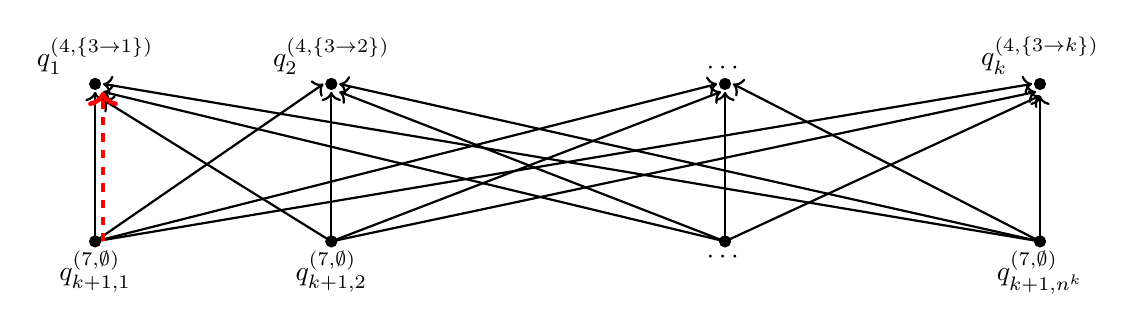
\begin{tikzpicture}
%%% The nodes represents the k query in the first round
\filldraw[black] (0, 2) circle (2pt) node [anchor=south]{$q_1^{(4, \{3 \to 1\} )}$};
\filldraw[black] (3, 2) circle (2pt) node [anchor=south]{$q_2^{(4, \{3 \to 2\} )}$};
% \filldraw[black] (6, 2) circle (2pt) node [anchor=south]{$q^4_3$};
\filldraw[black] (8, 2) circle (2pt) node [anchor=south]{$\cdots$};
\filldraw[black] (12, 2) circle (2pt) node [anchor=south]{$q_k^{(4, \{3 \to k\} )}$};
%%%%%% The nodes represents the n^k queries in the second round
\filldraw[black] (0, 0) circle (2pt) node [anchor=north]{$q_{k+1,1}^{(7, \emptyset)}$};
\filldraw[black] (3, 0) circle (2pt) node [anchor=north]{$q_{k+1,2}^{(7, \emptyset)}$};
% \filldraw[black] (6, 0) circle (2pt) node [anchor=north]{$q^{3, 7}_{k+1}$};
\filldraw[black] (8, 0) circle (2pt) node [anchor=north]{$\cdots$};
\filldraw[black] (12, 0) circle (2pt) node [anchor=north]{$q_{k+1,n^k}^{(7, \emptyset)}$};
%%%%%% The edges represents their dependency relations GROUP 1
\draw[ thick,->] (0, 0)  -- (0, 1.9) ;
\draw[ thick,->] (0, 0)  -- (2.9, 2) ;
% \draw[very thick,->] (0, 0)  -- (6, 2) ;
\draw[ thick,->] (0, 0)  -- (7.9, 2) ;
\draw[ thick,->] (0, 0)  -- (11.9, 2) ;
%%%%%% The edges represents their dependency relations GROUP 2
\draw[ thick,->] (3, 0)  -- (0.1, 1.8) ;
\draw[ thick,->] (3, 0)  -- (3, 1.9) ;
% \draw[very thick,->] (0, 0)  -- (6, 2) ;
\draw[ thick,->] (3, 0)  -- (7.95, 1.9) ;
\draw[ thick,->] (3, 0)  -- (11.95, 1.9) ;
%%%%%% The edges represents their dependency relations GROUP 3
\draw[ thick,->] (8, 0)  -- (0.1, 1.9) ;
\draw[ thick,->] (8, 0)  -- (3.1, 1.9) ;
% \draw[very thick,->] (0, 0)  -- (6, 2) ;
\draw[ thick,->] (8, 0)  -- (8, 1.9) ;
\draw[ thick,->] (8, 0)  -- (12, 1.85) ;
%%%%%% The edges represents their dependency relations GROUP 4
\draw[ thick,->] (12, 0)  -- (0.1, 2) ;
\draw[ thick,->] (12, 0)  -- (3.1, 2) ;
% \draw[very thick,->] (0, 0)  -- (6, 2) ;
\draw[ thick,->] (12, 0)  -- (8.1, 2) ;
\draw[ thick,->] (12, 0)  -- (12, 1.85) ;
%%%% The longest path representing the adaptivity
\draw[ultra thick, red, ->, dashed] (0.1, 0) -- (0.1, 1.9);
\end{tikzpicture}
}
\end{center}
\end{example}
%
\newpage

%
\begin{example}[Multi-Round Algorithm]
{
\[
MR \triangleq
\begin{array}{l}
    \left[i \leftarrow 1 \right]^1 ; \\
    \left[I \leftarrow [] \right]^2; \\
   \ewhile ~ [i < k]^{3} 
    \ ~ \edo ~ \\ \Big(
    \left[p \leftarrow c \right]^4 ; \\
    \left[a \leftarrow \query(p, I) \right]^5; \\
    \left[I \leftarrow \eupdt( {I}, (a, p))  \right]^6 ; \\
    \left[i \leftarrow i + 1 \right]^7 \\
    \Big) 
\end{array}
%
~~~~ \Rightarrow ~~~
%
MR^{ssa} \triangleq
\begin{array}{l}
    \left[i \leftarrow 1 \right]^1 ; \\
   \left[I \leftarrow [] \right]^2; \\
   \ewhile ~ [i < k]^{3} 0, [I_3,I_1,I_2] \\ 
    \ ~ \edo ~ \\ \Big(
    \left[p_1 \leftarrow c \right]^4 ; \\
    \left[a \leftarrow \query(p_1, I_2) \right]^5; \\
    \left[I_2 \leftarrow \eupdt( {I_3}, (a_1, p_1))  \right]^6;\\
    \left[i \leftarrow i + 1 \right]^7 \\
    \Big) 
\end{array}
\]
}
%
%
%
Adapt($MR$) = k.
\\
%
{
Using \THESYSTEM, we first generate a global list $G$ from an empty list $[]$ and empty whlemap $\emptyset$.
 \[[]; \emptyset; MR^{ssa} \to G; w  \land w = \emptyset\].
 %
 \[
 G_{k=2} = 
 \left[
 i_1^{1}, I_1^2, i_3^3, I_3^3, p_1^4, a_1^5, I_2^6, i_2^7
\right] 
\]
  We denote $I_1^{1}$ short for ${I_1}^{(1,\emptyset)}$ and ${I_3}^{(2,1)}$ short for ${I_3}^{(2,[2:1])}$, where the label $(2, 1)$ represents at line number $2$ and in the $1$ st iteration.
  }
{
	\[
M =  \left[ \begin{matrix}
   i_1^{1} & I_1^2 & i_3^3 & I_3^3 & p_1^4 & a_1^5 & I_2^6 & i_2^7\\
 0 & 0 & 0 & 0 & 0 & 0 & 0 & 0 \\
 1 & 0 & 0 & 0 & 0 & 0 & 0 & 0 \\
 0 & 0 & 0 & 0 & 0 & 0 & 0 & 0 \\
 0 & 1 & 0 & 0 & 0 & 0 & 0 & 0 \\
 0 & 1 & 1 & 1 & 0 & 0 & 0 & 0 \\
 1 & 0 & 0 & 0 & 1 & 0 & 0 & 0 \\
 0 & 0 & 0 & 0 & 0 & 0 & 0 & 0 \\
 0 & 0 & 0 & 0 & 0 & 1 & 0 & 0 \\
 0 & 0 & 0 & 0 & 0 & 1 & 1 & 1 \\
 1 & 0 & 0 & 0 & 0 & 0 & 0 & 0  \\
 \end{matrix} \right] 
~ , V = \left [ \begin{matrix}
i_1^1 & 0 \\
I_1^2 & 0 \\
i_3^3 & 2 \\
I_3^3 & 2 \\
p_1^4 & 2 \\
a_1^5 & 1 \\
I_2^6 & 2 \\
i_2^7 & 2
\end{matrix} \right ]
\]
}

\newpage
\begin{center}
%
\todo{
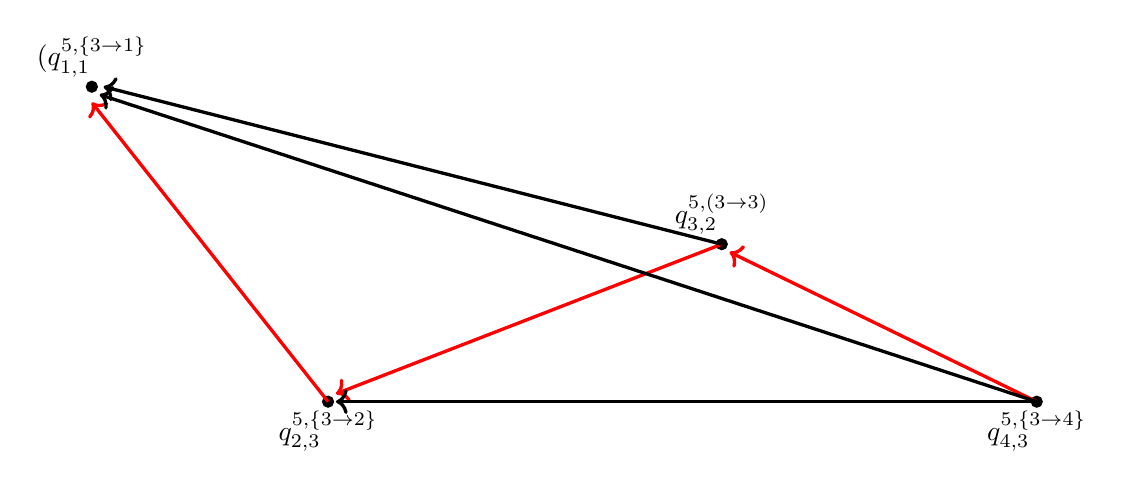
\begin{tikzpicture}
%%% The nodes represents the k query in the first round
\filldraw[black] (0, 4) circle (2pt) node [anchor=south]{$(q^{5, \{3 \to 1\}}_{1, 1}$};
\filldraw[black] (3, 0) circle (2pt) node [anchor=north]{$q^{5, \{3 \to 2\}}_{2, 3}$};
% \filldraw[black] (6, 0) circle (2pt) node [anchor=north]{$q^{3, 7}_{k+1}$};
% \filldraw[black] (8, 0) circle (2pt) node [anchor=north]{$\cdots$};
\filldraw[black] (12, 0) circle (2pt) node [anchor=north]{$q^{5, \{3 \to 4\}}_{4, 3}$};
\filldraw[black] (8, 2) circle (2pt) node [anchor=south]{$q^{5, (3 \to 3)}_{3, 2}$};
\draw[very thick,->, red] (3, 0)  -- (0, 3.8) ;
%
\draw[very thick,->, red] (8, 2)  -- (3.1, 0.1) ;
\draw[very thick,->] (8, 2)  -- (0.15, 4) ;
% \draw[very thick,->] (8, 0)  -- (3.1, 0) ;
% \draw[very thick,->] (8, 4)  -- (3, 0.2) ;
% %
%%%%%% The edges represents their dependency relations GROUP 4
% \draw[very thick,->] (0, 0)  -- (6, 2) ;
% \draw[very thick,->] (12, 2)  -- (8.1, 2) ;
\draw[very thick,->, red] (12, 0)  -- (8.1, 1.9) ;
\draw[very thick,->] (12, 0)  -- (3.1, 0) ;
\draw[very thick,->] (12, 0)  -- (0.1, 3.9) ;
% \draw[very thick,->] (12, 4)  -- (8.1, 2.1) ;
% %
% \draw[very thick,->] (12, 2)  -- (8.1, 0.1) ;
% \draw[very thick,->] (12, 0)  -- (8.1, 0) ;
% \draw[very thick,->] (12, 4)  -- (8, 0.2) ;
% %
% \draw[very thick,->] (12, 2)  -- (8.1, 3.9) ;
% \draw[very thick,->] (12, 0)  -- (8, 3.8) ;
% \draw[very thick,->] (12, 4)  -- (8.1, 4) ;
%
% \draw[very thick,->] (12, 2)  -- (8.1, 3.9) ;
%%%% The longest path representing the adaptivity
% \draw[ultra thick, red, ->, dashed] (3, 4.1)  -- (0.1, 4.1);
% \draw[ultra thick, red, ->, dashed] (8, 4.1)  -- (3.1, 4.1);
% \draw[ultra thick, red, ->, dashed] (12, 4.1)  -- (8.1, 4.1);
\end{tikzpicture}
}
\end{center}
%
\newpage
%
$\forall k. \forall D$, we have $A(TR^L) = (k - 1)$ given all possible execution traces.
\todo{
\begin{center}
%
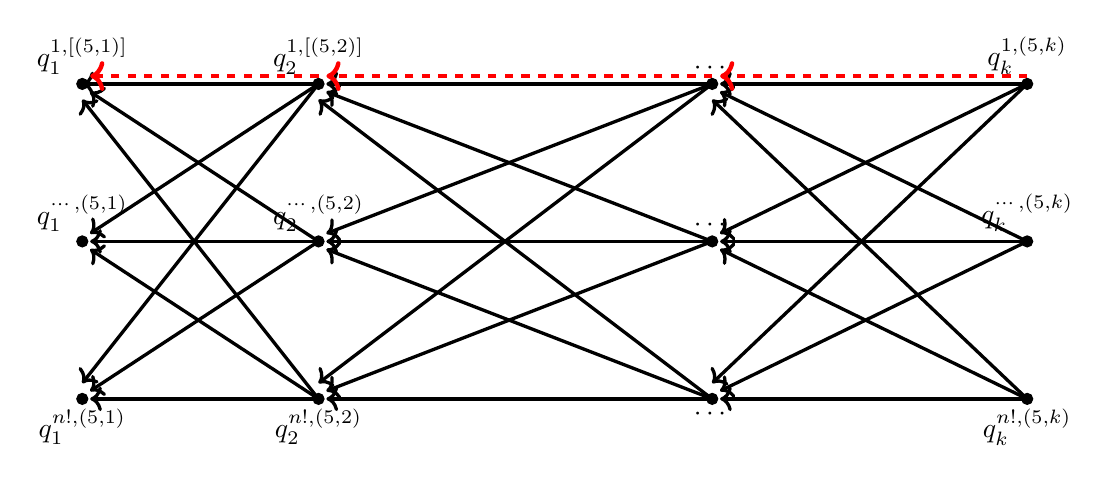
\begin{tikzpicture}
%%% The nodes represents the k query in the first round
\filldraw[black] (0, 4) circle (2pt) node [anchor=south]{$q^{1, [(5, 1)]}_1$};
\filldraw[black] (3, 4) circle (2pt) node [anchor=south]{$q^{1, [(5, 2)]}_2$};
% \filldraw[black] (6, 2) circle (2pt) node [anchor=south]{$q^4_3$};
\filldraw[black] (8, 4) circle (2pt) node [anchor=south]{$\cdots$};
\filldraw[black] (12, 4) circle (2pt) node [anchor=south]{$q^{1, (5, k)}_k$};
%%%%%% The nodes represents the n^k queries in the second round
\filldraw[black] (0, 0) circle (2pt) node [anchor=north]{$q^{n!, (5, 1)}_1$};
\filldraw[black] (3, 0) circle (2pt) node [anchor=north]{$q^{n!, (5, 2)}_2$};
% \filldraw[black] (6, 0) circle (2pt) node [anchor=north]{$q^{3, 7}_{k+1}$};
\filldraw[black] (8, 0) circle (2pt) node [anchor=north]{$\cdots$};
\filldraw[black] (12, 0) circle (2pt) node [anchor=north]{$q^{n!, (5, k)}_k$};
%%% The nodes represents the k query in the first round
\filldraw[black] (0, 2) circle (2pt) node [anchor=south]{$q^{\cdots, (5, 1)}_1$};
\filldraw[black] (3, 2) circle (2pt) node [anchor=south]{$q^{\cdots, (5, 2)}_2$};
% \filldraw[black] (6, 2) circle (2pt) node [anchor=south]{$q^4_3$};
\filldraw[black] (8, 2) circle (2pt) node [anchor=south]{$\cdots$};
\filldraw[black] (12, 2) circle (2pt) node [anchor=south]{$q^{\cdots, (5, k)}_k$};
%%%%%% The edges represents their dependency relations GROUP 1
\draw[very thick,->] (3, 2)  -- (0.1, 2) ;
\draw[very thick,->] (3, 0)  -- (0.1, 1.9) ;
\draw[very thick,->] (3, 4)  -- (0.1, 2.1) ;
%
\draw[very thick,->] (3, 2)  -- (0.1, 0.1) ;
\draw[very thick,->] (3, 0)  -- (0.1, 0) ;
\draw[very thick,->] (3, 4)  -- (0, 0.2) ;
%
\draw[very thick,->] (3, 2)  -- (0.1, 3.9) ;
\draw[very thick,->] (3, 0)  -- (0, 3.8) ;
\draw[very thick,->] (3, 4)  -- (0, 4) ;
% \draw[very thick,->] (0, 0)  -- (6, 2) ;
%%%%%% The edges represents their dependency relations GROUP 2
% \draw[very thick,->] (0, 0)  -- (6, 2) ;
\draw[very thick,->] (8, 2)  -- (3.1, 2) ;
\draw[very thick,->] (8, 0)  -- (3.1, 1.9) ;
\draw[very thick,->] (8, 4)  -- (3.1, 2.1) ;
%
\draw[very thick,->] (8, 2)  -- (3.1, 0.1) ;
\draw[very thick,->] (8, 0)  -- (3.1, 0) ;
\draw[very thick,->] (8, 4)  -- (3, 0.2) ;
%
\draw[very thick,->] (8, 2)  -- (3.1, 3.9) ;
\draw[very thick,->] (8, 0)  -- (3, 3.8) ;
\draw[very thick,->] (8, 4)  -- (3.1, 4) ;
%%%%%% The edges represents their dependency relations GROUP 4
% \draw[very thick,->] (0, 0)  -- (6, 2) ;
\draw[very thick,->] (12, 2)  -- (8.1, 2) ;
\draw[very thick,->] (12, 0)  -- (8.1, 1.9) ;
\draw[very thick,->] (12, 4)  -- (8.1, 2.1) ;
%
\draw[very thick,->] (12, 2)  -- (8.1, 0.1) ;
\draw[very thick,->] (12, 0)  -- (8.1, 0) ;
\draw[very thick,->] (12, 4)  -- (8, 0.2) ;
%
\draw[very thick,->] (12, 2)  -- (8.1, 3.9) ;
\draw[very thick,->] (12, 0)  -- (8, 3.8) ;
\draw[very thick,->] (12, 4)  -- (8.1, 4) ;
%
%%%% The longest path representing the adaptivity
\draw[ultra thick, red, ->, dashed] (3, 4.1)  -- (0.1, 4.1);
\draw[ultra thick, red, ->, dashed] (8, 4.1)  -- (3.1, 4.1);
\draw[ultra thick, red, ->, dashed] (12, 4.1)  -- (8.1, 4.1);
\end{tikzpicture}
\end{center}
}
\end{example}
% %
\section{Analysis of Generalization Error}

\begin{example}[Two Round Algorithm]
\[
TR^H(k) \triangleq
{
\begin{array}{l}
    % \left[j \leftarrow 0 \right]^1 ; \\
    \clabel{a_1 \leftarrow [] }^1; \\
    \eloop ~ [k]^{2} ~ (a_2 \leftarrow f(1, a_1, a_3)) \\
    ~ \edo ~ \\
    \Big(
     \clabel{x_1 \leftarrow \query() }^3 ; \\
    \clabel{a_3 \leftarrow x_1 :: a_2 }^4     \Big);\\
    \clabel{l \leftarrow q_{k + 1}(a_3)}^{5}\\
\end{array}
}
\]
\end{example}
%
\begin{example}[Multi-Round Algorithm]
\[
MR^H \triangleq
\begin{array}{l}
    %  \left[j \leftarrow 0 \right]^1 ; \\
    \left[I_2 \leftarrow [] \right]^1; \\
    \eloop ~ [k]^{2} ~ (I_2 \leftarrow f(2, I_1, I_3)) \\ 
    \ ~ \edo ~ \\ \Big(
    \left[p_1 \leftarrow c \right]^3 ; \\
    \left[a_1 \leftarrow \delta(\query(p, I_2)) \right]^4; \\
    \left[I_3 \leftarrow \eupdt( {I_2}, (a_1, p))  \right]^5
    \Big) 
\end{array}
\]
\end{example}
%
%
By applying different mechanisms $\delta()$ over the queries $\query(\cdot)$, we have different error bounds.
\\
\textbf{Gaussian Mechanism:} $N(0, \sigma)$ \cite{dwork2015preserving}:
\\
Adaptivity $r = 2$: 
$ \sigma = O \left(\frac{\sqrt{r \log(k)}}{\sqrt{n}} \right)$ (also known as expected error);
\\
Adaptivity unknown:
$ \sigma = O\left(\frac{\sqrt[4]{k}}{\sqrt{n}} \right)$;
\\
{Mean Squared Error Bound:} 
$ \frac{1}{2n} \min\limits_{\lambda \in [0, 1]}
\left( \frac{2\rho k n - \ln(1 - \lambda)}{\lambda} 
\right)
+ 2 \mathbb{E}_{Z_i \sim N(0, \frac{1}{2n^2 \rho})}
\left[ \max\limits_{i \in [k]} (Z_i^2) \right]$
%
\\
{Confidence Bounds:} minimize $\tau$ where
$\tau \geq \sqrt{\frac{2}{n \beta}
\min\limits_{\lambda \in [0, 1]}
\left( \frac{2\rho k n - \ln(1 - \lambda)}{\lambda} 
\right)
}$
and 
$\tau \geq \frac{2}{n} \sqrt{\frac{\ln(4n /\beta}{\rho'}}$ with confidence level $1 - \beta$ .
\\
\textbf{$(\epsilon, \delta)-DP$ mechanism}:
\\
Confidence Bounds:
$\tau \geq \sqrt{\frac{48}{n} \ln(4/\beta) }$ with $\epsilon \leq \frac{\tau}{4}$ and $\delta = 
\exp \left(\frac{-4 \ln (8/\beta)}{\tau} \right)$
\\
\textbf{Sample Splitting}: 
\\
Expected Error: $O \left(\frac{\sqrt{k \log(k)}}{\sqrt{n}} \right)$
\\
\textbf{Thresholdout}: $B, \sigma, T, h$ 
\\
Confidence bounds:  
$\tau = \max\limits\left\{ 
\sqrt{\frac{2\zeta }{h \beta}},
2\sigma \ln(\frac{\beta}{2}),
\sqrt{\frac{1}{\beta}} \cdot \left(\sqrt{T^2 + 56\sigma^2} + \sqrt{\frac{\zeta}{4h} } \right)
\right\}
$,
for $\zeta = \min\limits_{\lambda \in [0, 1)}
\left( \frac{2B \ (\sigma^2 h) - \ln(1 - \lambda)}{\lambda} \right)$

\clearpage

\section{new \THESYSTEM with loop }
\subsection{Analysis Rules/Algorithms of \THESYSTEM}

There are two steps for our algorithm to get the estimation of the adaptivity of a program $\ssa{c}$ in the ssa form. 
\begin{enumerate}
    \item Estimate the variables that are new generated (via assignment) and store these variables in a global list $G$. We have the algorithm of the form : $\ag{ G;w; \ssa{c}}{G';w'} $.
    \item We start to track the dependence between variables in a matrix $M$, whose size is $|G| \times |G|$, and track whether arbitrary variable is assigned with a query result in a vector $V$ with size $|G|$. The algorithm to fill in the matrix is of the form: $\ad{\Gamma ; \ssa{c} ; i_1}{M;V;{i_2}}$. $\Gamma$ is a vector records the variables the current program $\ssa{c}$ depends on, the index $i_1$ is a pointer which refers to the position of the first new-generated variable in $\ssa{c}$ in the global list $G$, and $i_2$ points to the first new variable that is not in $\ssa{c}$ (if exists). 
\end{enumerate}

% We have the judgment of the form $\vdash^{i_1, i_2}_{M,V} ~ c  $.  Our grade is a combination of a matrix $M$, used to track the dependency of variables appeared in the statement $c$, and a vector $V$ indicating the variables associated with results from queries $q$. The size of the matrix $M$ is $L \times L$, and vector $V$ of size $L$, where $L$ is the total size of variables needed in the program $c$, which is fixed per program. We assume the program is in the style of Static Single Assignment.To be more specific, we give a quick example: $x \leftarrow e_1; x \leftarrow e_2 $ will be rewritten as $ x_1 \leftarrow e_1; x_2 \leftarrow e_2$. And the if condition $ \eif ~ e_b \ethen x \leftarrow e_1 \eelse x \leftarrow e_2  $ will look like $ \eif ~ e_b \ethen x_1 \leftarrow e_1 \eelse x_2 \leftarrow e_2  $. As we have seen, SSA requires unique variables, and these newly generated variables will be recorded in the matrix $M$.  Also, the variable at different iteration is treated as different variable in the matrix $M$ and vector $V$.

% The superscript $i_1,i_2$  specify the range of "living" or "active" variables in the matrix and vector. $i_1$ is the starting line (and column) in the matrix where the new generated variables in program $c$ starts to show up. Likewise, $i_2$ states the ending position of active range by $c$.
%  Worth to mention, $i_1,i_2$ can be used to track the exact location of newly generated variables. For example, the assignment statement $x \leftarrow e$ or $x \leftarrow q $ with $c_2 =c_1+1$, tells us the variable $x$ is at the $c_1$th line(column) of the matrix. As we can notice, the loop increases the variables needed in the matrix by $N \times a$ where $N$ is the number of rounds of the loop and $a$ is the size of the variables generated in the loop body. We will have a global map, which maps the variable name to the position in the vector. We call it $GM: VAR \to \mathbb{N}$.

We give an example of $M$ and $V$ of the program $c$.   
$$
c= \begin{array}{c}
\ssa{\assign {x_1} {q}} ;        \\
\ssa{\assign {x_2} {x_1+1}} ;\\
\ssa{\assign {x_3} {x_2+2} }
\end{array}~~~~~~~~~~~~
M =  \left[ \begin{matrix}
 & (x_1) & (x_2) & (x_3) \\
(x_1) & 0 & 0 & 0 \\
(x_2) & 1 & 0 & 0 \\
(x_3) & 1 & 1 & 0 \\
\end{matrix} \right] ~ , V = \left [ \begin{matrix}
(x_1) &  1 \\
(x_2) & 0 \\
(x_3) & 0 \\
\end{matrix} \right ]
$$
Still use the program $c$ as the example, the global list $G$ is now : $ [ x_1 , x_2 , x_3] $. 
The function $\mathsf{Left}$ and $\mathsf{Right}$ is used to generate the corresponding vector of the left side and right side of an assignment. Take $\assign {x_2} {x_1+1} $ as an example, the result is shown as follows.
\[
\sf{L}(1) = \left[ \begin{matrix}
 0  & ~~~(x_1) \\
 1 & ~~~(x_2) \\
 0 & ~~~(x_3) \\
\end{matrix}   \right ] ~~~~~~~~~~~~~~
\sf{R} (x_1+1, 1) = \left[ \begin{matrix} 
   1 & 0 & 0 \\
   (x_1) & (x_2) & (x_3) \\
\end{matrix}  \right]
\]
Now let us think about the loop.
\[\ssa{c_3} \triangleq
\begin{array}{l}
     \left[\ssa{ x_1 \leftarrow q_1}  \right]^1 ; \\
    \eloop ~ [2]^{2} , 0,\\
  \ssa{[x_3 , x_1 , x_2]} 
     ~ \edo
    \\
    ~ \Big( 
    \left[\ssa{ y_1 \leftarrow q_2} \right]^3; \\
    \left[\ssa{x_2 \leftarrow y_1  + x_3 } \right]^5
    \Big) ; \\
     \left[ \assign{z_1}{x_3 + 2}  \right]^{6}
\end{array}
~~~~~~~~~~~~
M =  \left[ \begin{matrix}
 & (x_1) & (x_3^{1}) & (y_1^{1}) & (x_3^{1})  & (x_3^{2}) & (y_1^{2}) & (x_2^{2}) & (x_3^{f}) &  (z_1) \\
(x_1) & 0 & 0 & 0 & 0 & 0 & 0 & 0 &0 &0 \\
(x_3^{1}) & 1 & 0 & 0 & 0 & 0 & 0 & 0&0&0\\
(y_1^{1}) & 0 & 0 & 0 & 0 & 0 & 0& 0& 0 &0\\
(x_2^{1}) & 0 & 1 & 1 & 0 & 0 & 0 & 0& 0&0\\
(x_3^{2}) & 0 & 0 & 0 & 1 & 0 & 0 & 0 & 0&0 \\
(y_1^{2}) & 0 & 0 & 0 & 0 & 0 & 0 & 0& 0&0\\
(x_2^{2}) & 0 & 0 & 0 & 0 & 1 & 1 & 0& 0&0\\
(x_3^{f}) & 1 & 0 & 0 & 0 & 0 & 0 & 1& 0&0\\
(z_1) & 0 & 0 & 0 & 0 & 0 & 0 & 0 & 1 &0 \\
\end{matrix} \right] ~ , V = \left [ \begin{matrix}
(x_1) &  1 \\
(x_3^{1}) & 0 \\
(y_1^{1}) & 1 \\
(x_2^{1}) &  0 \\
(x_3^{2}) & 0 \\
(y_1^{2}) & 1 \\
(x_2^{2}) &  0 \\
(x_3^{f}) &  0 \\
(z_1) &  0 \\
\end{matrix} \right ]
\]

\[\ssa{c_3'} \triangleq
\begin{array}{l}
     \left[\ssa{ x_1 \leftarrow q_1}  \right]^1 ; \\
    \eloop ~ [0]^{2} , 0,\\
  \ssa{[x_3 , x_1 , x_2]} 
     ~ \edo
    \\
    ~ \Big( 
    \left[\ssa{ y_1 \leftarrow q_2} \right]^3; \\
    \left[\ssa{x_2 \leftarrow y_1  + x_3 } \right]^5
    \Big) ; \\
    \left[ \assign{z_1}{x_3 + 2}  \right]^{6}
\end{array}
~~~~~~~~~~~~
M =  \left[ \begin{matrix}
 & (x_1) & (x_3^{f}) & (z_1)  \\
(x_1) & 0 & 0 & 0 \\
(x_3^{f}) & 1 & 0 & 0 \\
(z_1^{2}) & 0 & 1 & 0 \\
\end{matrix} \right] ~ , V = \left [ \begin{matrix}
(x_1) &  1 \\
(x_3^{f}) & 0 \\
(z_1) &  0 \\
\end{matrix} \right ]
\]
We can now look at the if statement.
\[ c_4 \triangleq
\begin{array}{l}
   \left[ x \leftarrow q_1 \right]^1; \\
   \left[y \leftarrow q_2\right]^2 ; \\
    \eif \;( x + y == 5 )^3\; \\
    \mathsf{then} \;\left[ x \leftarrow q_3 \right]^4 \; \\
    \mathsf{else} (\;\left[ x \leftarrow q_4 \right]^5 ; \\
    y \leftarrow 2 ) ;\\
   \left[ z \leftarrow x +y \right]^6; \\
\end{array}
\hspace{20pt} \hookrightarrow \hspace{20pt}
%
 \ssa{c_4} \triangleq
\begin{array}{l}
   \left[ \ssa{ x_1 \leftarrow q_1} \right]^1; \\
   \left[\ssa{ y_1 \leftarrow q_2} \right]^2 ; \\
    \eif \;( \ssa{ x_1 + y_1 == 5} )^3, [ x_4,x_2,x_3 ],[] ,[y_3,y_1,y_2 ]\; \\
    \mathsf{then} \;\left[ \ssa{ x_2 \leftarrow q_3}\right]^4 \; \\
    \mathsf{else} (\;\left[ \ssa{x_3 \leftarrow q_4} \right]^5 ; \\
     \ssa{y_2 \leftarrow 2} ) \\
   \left[ \ssa{ z_1 \leftarrow x_4 +y_3 }\right]^6; \\
\end{array}
\]
\[
M_{c4} =  \left[ \begin{matrix}
 & (x_1) & (y_1) & (x_2) & (x_3)  & (y_2) & (x_4) & (y_3) & (z_1)  \\
(x_1) & 0 & 0 & 0 & 0 & 0 & 0 & 0 &0  \\
(y_1) & 0 & 0 & 0 & 0 & 0 & 0 & 0&0\\
(x_2) & 0 & 0 & 0 & 0 & 0 & 0& 0& 0 \\
(x_3) & 0 & 0 & 0 & 0 & 0 & 0 & 0& 0\\
(y_2) & 0 & 0 & 0 & 0 & 0 & 0 & 0 & 0 \\
(x_4) & 0 & 0 & 1 & 1 & 0 & 0 & 0 &0\\
(y_3) & 0 & 1 & 0 & 0 & 1 & 0 & 0 &0\\
(z_1) & 0 & 0 & 0 & 0 & 0 & 1 & 1 & 0  \\
\end{matrix} \right] ~ , V_{c4} = \left [ \begin{matrix}
(x_1) &  1 \\
(y_1) & 1 \\
(x_2) & 1 \\
(x_3) &  1 \\
(y_2) & 0 \\
(x_4) & 0 \\
(y_3) &  0 \\
(z_1) &  0 \\
\end{matrix} \right ]
\]
% We consider to have the superscript to denote the iteration number (or map if we have nested loop), as shown in the above matrix and vector. The global map $G$ is generated by analysing the program. We can estimate the variables needed in the loop by using the loop number $N$ and the loop body. In this example, the global map for $c_3$ : $ \{ x_1 \to 1, x_2^{1} \to 2, y_1^{1} \to 3 , x_3^{1} \to 4 , x_2^{2} \to 5 , y_1^{2} \to 6 , x_3^{2} \to 7  \} $.  
% By default, $G(x_2)$ gives the location for the first appearance of the variable $x_2$. We can also allow $G(x_2 , 2)$ to get the location of the second iteration $x_2^{2}$. We also allow $G(x, i, i+n)$ to return a set of locations where $x$ appears in the vector in the certain range $[i, i+n]$, which helps to locate variables in the loop.




% Also, to be able to track the relation between variables in varied iterations in the loop. we define a dependent map $\mathsf{DM}$ based on command $c$ to provide the dependency relation(syntactically) between variables. $\mathsf{VAR}(\expr)$ gives the set of variables appears in the expression $\expr$.
% \[
% \begin{array}{lll}
% \mathsf{DM} (c_1; c_2) & \triangleq &  \mathsf{DM} (c_1) \uplus \mathsf{DM} (c_2)  \\
% \mathsf{DM} (x_1 \leftarrow \expr ) & \triangleq & \{  x_1 \to \mathsf{VARS}(\expr)  \}
% \end{array}
% \]

\subsection{The algorithm to estimate the matrix and vector}
We first generate a list of variables $G$ that will be assigned with values (via the command $\assign{x}{e}$ or $\assign{x}{q}$). 

 \begin{mathpar}
\inferrule
{
}
{ \ag{G ;w; \ssa{[\assign {x}{\expr}]^{l}}}{G ++ [\ssa{x}^{(l,w)}];w}
% G ;w; \ssa{[\assign {x}{\expr}]^{l}} \to G ++ [x^{(l,w)}];w 
}
~\textbf{ag-asgn}
\and
\inferrule
{
}
{ \ag{G ;w;  [ \assign{\ssa{x}}{q(\ssa{\expr})}]^{l}}{  G ++ [\ssa{x}^{(l,w)}] ; w} 
}~\textbf{ag-query}
%
\and 
%
\inferrule
{
\ag{G; w; \ssa{c_1}}{  G_1;w_1}
\and 
 \ag{G_1;w ; \ssa{c_2}}{  G_2; w_2}
 \\
 {G_3 = G_2 ++ \ssa{[\bar{x}^{(l,w)}]++ \ssa{[\bar{y}^{(l,w)}]}++ \ssa{[\bar{z}^{(l,w)}]} }}
}
{
\ag{G; w;
[\eif(\ssa{\bexpr},[ \bar{\ssa{x}}, \bar{\ssa{x_1}}, \bar{\ssa{x_2}}] ,[ \bar{\ssa{y}}, \bar{\ssa{y_1}}, \bar{\ssa{y_2}}],[ \bar{\ssa{z}}, \bar{\ssa{z_1}}, \bar{\ssa{z_2}}], \ssa{ c_1, c_2)}]^{l} }{ G_3 ;w}
}~\textbf{ag-if}
%
%
%
\and 
%
\inferrule
{
\ag{G; w; \ssa{c_1}}{ G_1; w_1}
\and 
\ag{G_1;w_1; \ssa{c_2}}{ G_2; w_2}
}
{
\ag{G; w;
\ssa{(c_1 ; c_2)}}{  G_2 ; w_2}
}
~\textbf{ag-seq}
\and 
\inferrule
{
{G_0 = G \quad w_0 =w }
\and
\forall 0 \leq z < N. 
{ \ag{ G_z ++ \ssa{[\bar{x}^{(l, {w_z}+l)}]} ; (w_z+l); \ssa{c}}{ G_{z+1} ; w_{z+1}}  }
\\
{G_f = G_N ++ \ssa{[\bar{x}^{(l, w_N \setminus l)}]} }
\and
{ \ssa{\aexpr} =  {N}  }
}
{\ag{G; w; [\eloop ~ \ssa{\aexpr}, n, [\bar{\ssa{x}}, \bar{\ssa{x_1}}, \bar{\ssa{x_2}}] ~ \edo ~ \ssa{c}]^{l} }{ G_f; w_N\setminus l }
}~\textbf{ag-loop}
\end{mathpar}


%
%
% \paragraph{Analysis Rules.}
% \[\begin{array}{ll}
%     \mathcal{A}( \assign x \expr )( \Gamma , i )  & =  ( \mathsf{L}(x) * ( \mathsf{R}(\expr) + \Gamma ), V, i+1 )\\
%     \mathcal{A}( \assign x q)( \Gamma ,  i )  & = ( \mathsf{L}(x) * ( \mathsf{R}(\emptyset) + \Gamma) , \mathsf{L}(x) , i+1 )\\
%     \mathcal{A}( \eif ~ e_b \ethen c_1 \eelse c_2 )( \Gamma , i ) & =   \elet \; (M_1, v_1, i_1) =  \mathcal{A}(C_1)(\Gamma +\mathsf{R}(e_b) , i)
%     \ein \; \\
%     &  \elet \;  (M_2, v_2, i_2)= \mathcal{A}(C_2) (\Gamma +\mathsf{R}(e_b) ,i_1) \ein \; \\
%     & (  M_1 \uplus M_2, V_1 \uplus V_2   , i_2 )
%     \\
%     \mathcal{A}( c_1 ; c_2 )( \Gamma ,  i )  & =  \elet \;     (M_1, v_1, i_1) = 
%     \mathcal{A}(c_1) (\Gamma  +\mathsf{R}(e_b) , i)
%     \ein \; \\
%     &  \elet \;  (M_2, v_2, i_2) =                      \mathcal{A}(c_2)(\Gamma +\mathsf{R}(e_b) ,
%       i_1) \ein \; \\ 
%       & (  M_1 \cdot M_2, V_1 \uplus V_2   , i_2 )    \\
%      \mathcal{A}( \eloop ~ \expr_N ~ (c_1) ~ \edo ~ c_2  )( \Gamma ,  i )  & =  \elet \;     (M_1, v_1, i+a) = 
%     \mathcal{A}(c_1;c_2 ) (\Gamma , i)
%     \ein \; \\
%     & ( M_{i,a}^N(c_1), V_{i, a}^N , i + N*a ) \\
%  \mathcal{A}( \eswitch(\expr, x,(v_j \rightarrow q_j )  )( \Gamma ,  i+j )  & =  \elet \;     (M_j, v_j, i+j) = 
%     \mathcal{A}(x_j \leftarrow q_j ) (\Gamma + \mathsf{R}(e), i+j-1)     
%   \ein \\
%   & ( \sum_{j=0}^{N} M_j, \sum_{j=0}^{N} V_j, i + N ) \quad j \in \{1, \dots, N\}  \\
%     \end{array}
% \]
%
%
\paragraph{Analysis Logic Rules.}
%
%
$\Gamma$ is a matrix of one row and $N$ columns, $N = |G|=|V|$.\\ 

$\mathsf{L(i)}$ generates a matrix of one column, $N$ rows, where the $i-th$ row is $1$, all the other rows are $0$.\\

$\mathsf{R(e, i)}$ generates a matrix of one row and $N$ columns, where the locations of variables in $e$ is marked as $1$. To handle loop, for instance, the variable $y$ appears many times in $G$, the argument $i$ helps to find the location of the current living variable $y$ in the expression $e$, which is the latest $y$ with the largest location $i_y< i$ in our global variable list $G$.\\ 


{$ \forall 0 \leq z < |\bar{x}|. \bar{x}(z) = x_z, \bar{x_1}(z) = x_{1z}, \bar{x_2}(z) = x_{2z} $ } \\

$ \Gamma \vdash_{M,v_{\emptyset}}^{i, i+ |\ssa{\bar{x}}|} \ssa{[ \bar{x},\bar{x_1},\bar{x_2}   ]} \triangleq { \forall 0 \leq z < |\bar{x}|.  \Gamma \vdash_{M_{x_z}, V_{\emptyset}}^{i+z, i+z+1 } x_z \leftarrow x_{1z} + x_{2z} }$ where $M = \sum_{z\in [|\bar{x}|] }M_{x_z} $\\

\framebox{$ {\Gamma} \vdash^{i_1, i_2}_{M,V} ~ c $}
%
% \begin{mathpar}
% \inferrule
% {M = \mathsf{L}(i) * ( \mathsf{R}(\expr,i) + \Gamma )
% }
% {\Gamma \vdash_{M, V_{\emptyset}}^{(i, i+1)} [\assign {\ssa{x}}{\ssa{\expr}} ]^{l}
% }
% ~\textbf{asgn}
% \and
% \inferrule
% {M = \mathsf{L}(i) * ( \Gamma)
% \\
% V= \mathsf{L}(i)
% }
% { \Gamma \vdash^{(i, i+1)}_{M, V} [ \assign{\ssa{x}}{q} ]^{l} 
% }~\textbf{query}
% %
% \and 
% %
% \inferrule
% {
% \Gamma + \mathsf{R}(\bexpr, i_1) \vdash^{(i_1, i_2)}_{M_1, V_1} \ssa{c_1} 
% % : \Phi \land \bexpr \Rightarrow \Psi
% \and 
% \Gamma + \mathsf{R}(\bexpr, i_1) \vdash^{(i_2, i_3)}_{M_2, V_2} \ssa{c_2} 
% % : \Phi \land \neg \bexpr \Rightarrow \Psi
% \\
% { \forall 0 \leq j < |\bar{x}|. \bar{x}(j) = x_j, \bar{x_1}(j) = x_{1j}, \bar{x_2}(j) = x_{2j}  }
% \\
% { \forall 0 \leq j < |\bar{x}|.  \Gamma \vdash_{M_{x_j}, V_{\emptyset}}^{i_3+j, i_3+j+1 } x_j \leftarrow x_{1j} + x_{2j} }
% \and
% { \forall 0 \leq j < |\bar{y}|.  \Gamma \vdash_{M_{y_j}, V_{\emptyset}}^{i_3+|\bar{x}|+j, i_3+|\bar{x}|+j+1 } y_j \leftarrow y_{1j} + y_{2j} }
% \\
% { \forall 0 \leq j < |\bar{z}|.  \Gamma \vdash_{M_{z_j}, V_{\emptyset}}^{i_3+|\bar{x}|+|\bar{y}|+j, i_3+|\bar{x}|+|\bar{y}|+j+1 } z_j \leftarrow z_{1j} + z_{2j} }
% \and
% {M = (M_1+M_2)+ \sum_{j\in [|\bar{x}|] }M_{x_j} + \sum_{j\in [|\bar{y}|] }M_{y_j} + \sum_{j\in [|\bar{z}|] }M_{z_j} }
% }
% {
% \Gamma \vdash^{(i_1, i_3+|\bar{x}|+|\bar{y}|+|\bar{z}|)}_{M, V_1 \uplus V_2 } 
% [\eif(\sbexpr,[ \bar{\ssa{x}}, \bar{\ssa{x_1}}, \bar{\ssa{x_2}}] ,[ \bar{\ssa{y}}, \bar{\ssa{y_1}}, \bar{\ssa{y_2}}] , [ \bar{\ssa{z}}, \bar{\ssa{z_1}}, \bar{\ssa{z_2}}] , \ssa{ c_1, c_2)}]^{l}
% }~\textbf{if}
% %
% %
% %
% \and 
% %
% \inferrule
% {
% \Gamma \vdash^{(i_1, i_2)}_{M_1, V_1} \ssa{c_1} 
% % : \Phi \Rightarrow \Phi_1
% \and 
% \Gamma \vdash^{(i_2, i_3)}_{M_2, V_2} \ssa{c_2} 
% % : \Phi_1 \Rightarrow \Psi 
% }
% {
% \Gamma \vdash^{(i_1, i_3)}_{M_1 \green{;} M_2, V_1 \uplus V_2}
% \ssa{c_1 ; c_2} 
% % : \Phi \Rightarrow \Psi
% }
% ~\textbf{seq}
% \and 
% \inferrule
% {
% B= |\ssa{\bar{x}}| 
% \and
% {\Gamma \vdash^{(i, i+B)}_{M_{10}, V_{10}} [\bar{\ssa{x}}, \bar{\ssa{x_1}}, \bar{\ssa{x_2}}] }
% \and
% {\Gamma \vdash^{(i+B,i+B+A )}_{M_{20}, V_{20}} \ssa{c} 
% }
% \\
% \forall 1 \leq j < N. 
% {\Gamma \vdash^{(i+j*(B+A), i+B+j*(B+A))}_{M_{1j}, V_{1j}}  } [\bar{\ssa{x}}, \bar{\ssa{x_1}}, \bar{\ssa{x_2}}]
% \and
% {\Gamma \vdash^{(i+B+j*(B+A),i+B+A+j*(B+A) )}_{M_{2j}, V_{2j}} \ssa{c} 
% % : \Phi \land e_n = \lceil{z+1}\rceil \Rightarrow \Psi 
% }
% \\
% {\Gamma \vdash^{(i+N*(B+A) ,i+N*(B+A)+B )}_{M, V} [\bar{\ssa{x}}, \bar{\ssa{x_1}}, \bar{\ssa{x_2}}]
% % : \Psi \Rightarrow \Phi \land e_N = \lceil{z}\rceil 
% }
% \and
% { \ssa{a} = \lceil {N} \rceil }
% \and
% {M' = M+ \sum_{0 \leq j <N} M_{1j}+M_{2j}  }
% \and
% {V' = V \uplus \sum_{0 \leq j <N} V_{1j} \uplus V_{2j}  }
% }
% {\Gamma \vdash^{(i, i+N*(B+A)+B   )}_{M', V'} 
% [\eloop ~ \ssa{\aexpr}, 0, [\bar{\ssa{x}}, \bar{\ssa{x_1}}, \bar{\ssa{x_2}}] ~ \edo ~ \ssa{c}]^{l}
% % : \Phi \land \expr_N = \lceil { N} \rceil \Rightarrow \Phi \land \expr_N = \lceil{0}\rceil
% }~\textbf{loop}
% % \and 
% % \inferrule
% % {
% % \Gamma \vdash^{(i,i+a )}_{M, V} c 
% % }
% % {\Gamma \vdash^{(i, i+ N*a)}_{M_{i,a}^N(f), V_{i, a}^N} 
% % \ewhile([\bexpr]^l,   c) : \phi \Rightarrow \psi
% % }~\textbf{while}
% %
% \and
% %
% \inferrule
% { \Gamma + \mathsf{R}(\expr,i) \vdash^{(i, i+1)}_{M, V} \assign{ x}{q_j} 
% % : \Phi \Rightarrow \Psi
% \\
% j \in \{1, \dots, N\}     }
% {\Gamma \vdash^{(i, i+1)}_{ M,V } 
% [\eswitch(\ssa{\expr}, \ssa{x},(v_j \rightarrow q_j ) ]^{l}
% % : \Phi \Rightarrow \Psi 
% }
% ~\textbf{switch}
% % %
% % \and
% % %
% % \inferrule
% % { 
% % \vDash 
% % \Phi \Rightarrow \Phi'  
% % \and
% % \Gamma \vdash^{(i_1, i_2)}_{(M',V')} c : \Phi' \Rightarrow \Psi'
% % \and
% % \vDash \Psi' \Rightarrow \Psi
% % \and 
% % \Phi \vDash M' \leq M
% % \and 
% % \Phi \vDash V' \leq V
% % }
% % {\Gamma \vdash^{(i_1, i_2)}_{(M,V)} c 
% % : \Phi \Rightarrow \Psi
% % }
% % ~\textbf{conseq}
% \end{mathpar}
\begin{mathpar}
\inferrule
{M = \mathsf{L}(i) * ( \mathsf{R}(\ssa{\expr},i) + \Gamma )
}
{
 \ad{\Gamma;[\assign {\ssa{x}}{\ssa{\expr}} ]^{l}; i }{M; V_{\emptyset}; i+1 }
% \Gamma \vdash_{M, V_{\emptyset}}^{(i, i+1)} [\assign {\ssa{x}}{\ssa{\expr}} ]^{l}
}
~\textbf{ad-asgn}
\and
\inferrule
{M = \mathsf{L}(i) * ( \mathsf{R}(\ssa{\expr},i) + \Gamma )
\\
V= \mathsf{L}(i)
}
{ 
\ad{\Gamma;[ \assign{\ssa{x}}{q(\ssa{\expr})} ]^{l} ; i }{M;V;i+1}
%  \vdash^{(i, i+1)}_{M, V} [ \assign{\ssa{x}}{q(\ssa{\expr})} ]^{l} 
}~\textbf{ad-query}
%
\and 
%
\inferrule
{
{\ad{\Gamma + \mathsf{R}(\ssa{\bexpr}, i_1); \ssa{c_1} ; i_1 }{ M_1;V_1;i_2 }}
% \Gamma + \mathsf{R}(\bexpr, i_1) \vdash^{(i_1, i_2)}_{M_1, V_1} \ssa{c_1} 
% : \Phi \land \bexpr \Rightarrow \Psi
\and 
{\ad{\Gamma + \mathsf{R}(\ssa{\bexpr}, i_1);\ssa{c_2} ; i_2 }{ M_2; V_2 ;i_3}}
% \Gamma + \mathsf{R}(\ssa{\bexpr}, i_1) \vdash^{(i_2, i_3)}_{M_2, V_2} \ssa{c_2} 
% : \Phi \land \neg \bexpr \Rightarrow \Psi
\\
% { \forall 0 \leq j < |\bar{x}|. \bar{x}(j) = x_j, \bar{x_1}(j) = x_{1j}, \bar{x_2}(j) = x_{2j}  }
{\ad{\Gamma; [ \bar{\ssa{x}}, \bar{\ssa{x_1}}, \bar{\ssa{x_2}}]; i_3 }{ M_x; V_{\emptyset}; i_3+|\bar{\ssa{x}}| }}
%
\and
%
{\ad{\Gamma; [ \bar{\ssa{y}}, \bar{\ssa{y_1}}, \bar{\ssa{y_2}}]; i_3+|\bar{\ssa{x}}| }{ M_y; V_{\emptyset}; i_3+|\bar{\ssa{x}}|+|\bar{\ssa{y}}| }}
%
\\
%
{\ad{\Gamma; [ \bar{\ssa{z}}, \bar{\ssa{z_1}}, \bar{\ssa{z_2}}]; i_3+|\bar{\ssa{x}}|+ |\bar{\ssa{y}}|}{ M_y; V_{\emptyset}; i_3+|\bar{\ssa{x}}|+|\bar{\ssa{y}}| + |\bar{\ssa{z}}| }}
\\
{M = (M_1+M_2)+ M_x+M_y +M_z }
}
{
\ad{\Gamma ; \eif([\ssa{\bexpr}]^{l},[ \bar{\ssa{x}}, \bar{\ssa{x_1}}, \bar{\ssa{x_2}}] ,[ \bar{\ssa{y}}, \bar{\ssa{y_1}}, \bar{\ssa{y_2}}] , [ \bar{\ssa{z}}, \bar{\ssa{z_1}}, \bar{\ssa{z_2}}] , \ssa{ c_1, c_2)} ; i_1}{ M ;V_1 \uplus V_2  ; i_3+|\bar{x}|+|\bar{y}|+|\bar{z}| }
}~\textbf{ad-if}
%
%
%
\and 
%
\inferrule
{
{\ad{\Gamma; \ssa{c_1} ; i_1 }{ M_1 ; V_1; i_2 }  }
% \Gamma \vdash^{(i_1, i_2)}_{M_1, V_1} \ssa{c_1} 
% : \Phi \Rightarrow \Phi_1
\and 
{\ad{\Gamma;\ssa{c_2}; i_2}{M_2; V_2 ;i_3 }}
% \Gamma \vdash^{(i_2, i_3)}_{M_2, V_2} \ssa{c_2} 
% : \Phi_1 \Rightarrow \Psi 
}
{
\ad{\Gamma ; (\ssa{c_1 ; c_2} ) ; i_1}{(M_1 {;} M_2) ; V_1 \uplus V_2 ; i_3  }
% \Gamma \vdash^{(i_1, i_3)}_{M_1 {;} M_2, V_1 \uplus V_2}
% \ssa{c_1 ; c_2} 
% : \Phi \Rightarrow \Psi
}
~\textbf{ad-seq}
\and 
\inferrule
{
B= |\ssa{\bar{x}}| \and {A = |\ssa{c}|}
% \and
% {\Gamma \vdash^{(i, i+B)}_{M_{10}, V_{10}} [\bar{\ssa{x}}, \bar{\ssa{x_1}}, \bar{\ssa{x_2}}] }
% \and
% {\Gamma \vdash^{(i+B,i+B+A )}_{M_{20}, V_{20}} \ssa{c} 
% }
\\
\forall 0 \leq j < N. 
{\ad{\Gamma;[\bar{\ssa{x}}, \bar{\ssa{x_1}}, \bar{\ssa{x_2}}]; i+ j*(B+A) }{M_{1j};V_{1j}; i+B+j*(B+A) }}
% {\Gamma \vdash^{(i+j*(B+A), i+B+j*(B+A))}_{M_{1j}, V_{1j}}  } [\bar{\ssa{x}}, \bar{\ssa{x_1}}, \bar{\ssa{x_2}}]
\\
{
\ad{\Gamma;\ssa{c} ; i+B+j*(B+A)  }{M_{2j}; V_{2j}; i+B+A+j*(B+A) }
% \Gamma \vdash^{(i+B+j*(B+A),i+B+A+j*(B+A) )}_{M_{2j}, V_{2j}} \ssa{c} 
% : \Phi \land e_n = \lceil{z+1}\rceil \Rightarrow \Psi 
}
\\
{
\ad{\Gamma ; [\bar{\ssa{x}}, \bar{\ssa{x_1}}, \bar{\ssa{x_2}}] ; i+N*(B+A) }{M; V ;i+N*(B+A)+B}
% \Gamma \vdash^{(i+N*(B+A) ,i+N*(B+A)+B )}_{M, V} [\bar{\ssa{x}}, \bar{\ssa{x_1}}, \bar{\ssa{x_2}}]
% : \Psi \Rightarrow \Phi \land e_N = \lceil{z}\rceil 
}
\\
{ \ssa{\aexpr} =  {N}  }
\and
{M' = M+ \sum_{0 \leq j <N}( M_{1j}+M_{2j})  }
\and
{V' = V \uplus \sum_{0 \leq j <N}( V_{1j} \uplus V_{2j})  }
}
{
\ad{\Gamma;\eloop ~ [\ssa{\aexpr}]^{l}, ~0, [\bar{\ssa{x}}, \bar{\ssa{x_1}}, \bar{\ssa{x_2}}] ~ \edo ~ \ssa{c}, i }{ M';V' ;i+N*(B+A)+B }
%  \vdash^{(i,   )}_{M', V'} 
% : \Phi \land \expr_N = \lceil { N} \rceil \Rightarrow \Phi \land \expr_N = \lceil{0}\rceil
}~\textbf{ad-loop}
\end{mathpar}
%
\begin{figure}
   \[
 \begin{array}{lll}
    |[\eswitch(\ssa{\expr}, \ssa{x},(v_j \rightarrow q_j )]^{l} |_{low}  &=& [\eswitch(|\ssa{\expr}|_{low}, |x|_{low},(v_j \rightarrow q_j )]^{l} \\
    | [\eloop ~ \ssa{\aexpr}, n, [\bar{\ssa{x}}, \bar{\ssa{x_1}}, \bar{\ssa{x_2}}] ~ \edo ~ \ssa{c}]^{l}|_{low}  &=& [\eloop ~ |\ssa{\aexpr}|_{low},  ~ \edo ~ |\ssa{c}|_{low}]^{l} \\
      |\ssa{c_1 ; c_2}|_{low}  &=& |\ssa{c_1}|_{low} ; |\ssa{c_2}|_{low} \\
       |[\eif(\sbexpr,[ \bar{\ssa{x}}, \bar{\ssa{x_1}}, \bar{\ssa{x_2}}] ,[ \bar{\ssa{y}}, \bar{\ssa{y_1}}, \bar{\ssa{y_2}}] , [ \bar{\ssa{z}}, \bar{\ssa{z_1}}, \bar{\ssa{z_2}}] , \ssa{ c_1, c_2)}]^{l}|_{low}  &=&
       [\eif(|\sbexpr|_{low}, |\ssa{ c_1}|_{low}, |\ssa{c_2}|_{low})]^{l}\\
       | [\assign {\ssa{x}}{\ssa{\expr}}]^{l}|_{low} & = & [\assign {|\ssa{x}|_{low}}{|\ssa{\expr}|_{low}} ]^{l}  \\
       | [\assign {\ssa{x}}{q} ]^{l} |_{low} & = & [\assign {|\ssa{x}|_{low}}{q}]^{l} \\
       |x_i|_{low} & = & x \\
       |n |_{low} & = & n \\
      | \ssa{\aexpr_1} \oplus_{a} \ssa{\aexpr_2} |_{low} & = &  |\ssa{\aexpr_1}|_{low} \oplus_a |\ssa{\aexpr_2}|_{low} \\
      | \ssa{\bexpr_1} \oplus_{b} \ssa{\bexpr_2} |_{low} & = &  |\ssa{\bexpr_1}|_{low} \oplus_b |\ssa{\bexpr_2}|_{low}
 \end{array}
\]
    \caption{The erasure of SSA}
    \label{fig:ssa_erasure}
\end{figure}


\[
\begin{array}{lll}
M_1 ; M_2 & := & M_2 \cdot M_1 + M_1 + M_2      \\
V_1 \uplus V_2 & := & \left\{
\begin{array}{ll}
1 & (V_1[i] = 1 \lor V_2[i] = 1) \land i = 1, \cdots, N \land |V_1| = |V_2|\\
0 & o.w.
\end{array}\right.\\
%
% M_1 \uplus M_2 & := & \left\{
% \begin{array}{ll}
% 1 & (M_1[i][j] = 1  \lor M_2[i][j] = 1) \land i, j = 1, \cdots, N \land |M_1| = |M_2|\\
% 0 & (M_1[i][j] = 0  \land M_2[i, j] = 0) \land i, j = 1, \cdots, N \land |M_1| = |M_2|\\
% \bot & o.w.
% \end{array}\right.\\
%
% V_{(i, a)}^N
% & := & \left\{
% \begin{array}{ll}
% V[i+ o*a, i + (o + 1) * a-1] = V[i, i + a-1] & 
%  o = 1, \cdots, N - 1 \\
% \bot & o.w.
% \end{array}\right.\\
% %
% M_{(i, a)}^N (c)
% & := & \left\{
% \begin{array}{ll}
% M[i+ o*a, i + (o + 1) * a-1][i + o*a, i + (o + 1) * a-1] & \\
% = M[i, i + a-1][i, i+ a-1] & 
%  o = 1, \cdots, N - 1 \\
% M[i+ o*a,i + (o + 1) * a-1][0, i + o * a-1] = 
% 0 & 
%  o = 1, \cdots, N - 1 \\
% M[0, i + o * a-1][i+ o*a, i + (o + 1) * a-1] & \\
% =  M[0, i + (o - 1) * a-1][i+ (o - 1)*a, i + o * a-1] & 
%  o = 1, \cdots, N - 1 \\
%  \qquad & \qquad  \qquad  \\
% M[l][k] = 
% 1& 
% \begin{array}{l}
% \forall x_l \in  \mathsf{DM}(c). \forall x_k \in  \mathsf{DM}(c)(x_l).\\
%  for \quad o = 0, \cdots, N . \\
% l \in G(x_l,i+ o*a, i+(o+1)*a-1) \land \\
% k \in G(x_k,0, i + (o ) * a-1) \land \\
% \end{array}\\
% \bot & o.w.
% \end{array}\right.\\
%
\end{array}
\]
%
% \begin{center}
% \begin{tabular}{p{15pt}|p{15pt}|p{15pt}||p{15pt}|p{15pt}
% |p{15pt}||p{15pt}|p{15pt}|
% p{15pt}|p{15pt}|p{15pt}|p{15pt}|p{15pt}| } 
%  1 & $\cdots$ & i-1 & i & $\cdots$ & \tiny{i+a-1} & {\tiny i+a } 
% & $\cdots$ & {\tiny{i+2a-1} }
% & $\cdots$ & {\tiny i+N*a-1} & {\tiny i+N*a} & $\cdots$ \\
% \hline
% $\cdots$  & \cellcolor{green} & \cellcolor{green} & \cellcolor{sandstorm} 0 & \cellcolor{sandstorm} 0 & \cellcolor{sandstorm} 0 & \cellcolor{sandstorm} 0 & \cellcolor{sandstorm} 0 & \cellcolor{sandstorm} 0 &  &  &  & \\[10pt]
% \hline
% i-1 & \cellcolor{green} & \cellcolor{green} & \cellcolor{sandstorm} 0 & \cellcolor{sandstorm} 0 & \cellcolor{sandstorm} 0 & \cellcolor{sandstorm} 0 &\cellcolor{sandstorm} 0 & \cellcolor{sandstorm} 0 &  &  &  &  \\ [10pt]
% \hline
% i & \cellcolor{periwinkle} & \cellcolor{periwinkle} & \cellcolor{pink} & \cellcolor{pink} &\cellcolor{pink} & \cellcolor{sandstorm} 0 &
% \cellcolor{sandstorm} 0 &
% \cellcolor{sandstorm} 0 &&&& \\ [10pt]
% \hline
% $\cdots$ & \cellcolor{periwinkle} & \cellcolor{periwinkle}
% &\cellcolor{pink} &\cellcolor{pink}&\cellcolor{pink} &
% \cellcolor{sandstorm} 0 & \cellcolor{sandstorm} 0 &
% \cellcolor{sandstorm} 0 &&&& \\ [10pt]
% \hline
% i+a-1 &\cellcolor{periwinkle} &\cellcolor{periwinkle} & \cellcolor{pink} & \cellcolor{pink} & \cellcolor{pink} 
% & \cellcolor{sandstorm} 0 & \cellcolor{sandstorm} 0 
% & \cellcolor{sandstorm} 0 &&&& \\ [10pt]
% \hline \hline
% {\scriptsize i+a }  & \cellcolor{periwinkle} & \cellcolor{periwinkle} & \cellcolor{trueblue} &\cellcolor{trueblue}
% & \cellcolor{trueblue}& \cellcolor{pink} 
% &\cellcolor{pink} & \cellcolor{pink} & &&& \\ [10pt]
% \hline
% $\cdots$ &\cellcolor{periwinkle} &\cellcolor{periwinkle} & \cellcolor{trueblue}  & \cellcolor{trueblue} c & \cellcolor{trueblue} 
% & \cellcolor{pink} & \cellcolor{pink} &\cellcolor{pink} 
% &&&& \\ [10pt]
% \hline
% {\small i+2a-1 } &\cellcolor{periwinkle} & \cellcolor{periwinkle} & \cellcolor{trueblue} 
% & \cellcolor{trueblue}  & \cellcolor{trueblue}
% & \cellcolor{pink} & \cellcolor{pink} & \cellcolor{pink} 
% &&&& \\ [10pt]
% \hline
% $\cdots$ & &&&&&&&&&&&  \\ [10pt]
% \hline
% {\tiny i+N*a-1 } & &&&&&&&&&&& \\ [10pt]
% \hline
% {\tiny i+N*a} & &&&&&&&&&&&\\ [10pt]
% \hline
% $\cdots$ & &&&&&&&&&&&\\ [10pt]
% \hline
% \end{tabular}
% \end{center}
%
%
%
       
% \begin{defn}
% [Validity of hoare triple]
% If $ c : \psi \Rightarrow \phi$, for any memory $m$ and database $D$ s.t., $\psi(m)$ holds, for any trace $t$, loop maps $w$ so that $ \config{m, c, t,w} \rightarrow^{*} \config{m', \eskip, t', w'}$, then $\phi(m')$ holds, written $\vDash c : \psi \Rightarrow \phi $.  
% \end{defn}




\newpage
\bibliographystyle{plain}
\bibliography{adaptivity.bib}

\end{document}



